%!TEX root = ../PhD_thesis__Edouard_Leurent
% Set counter to define 1st miniTOC.
\setcounter{mtc}{-1}
% FIXME change here if this issue happens again https://github.com/Naereen/phd-thesis/issues/4
\adjustmtc
% List of included chapters goes here


%!TEX root = ../../PhD_thesis__Edouard_Leurent.tex

\graphicspath{{2-Chapters/1-Chapter/}}

\chapter{Introduction}
\label{chapter:1}

\begin{flushright}
	\begin{tabular}{@{}l@{}}
%		\emph{What we call the beginning is often the end}\\
%		\hdashline
		\emph{We shall not cease from exploration}\\
		\emph{And the end of all our exploring}\\
		\emph{Will be to arrive where we started}\\
		\emph{And know the place for the first time.}\\
	\end{tabular}
	
	%T. S. Eliot, \href{https://eleurent.github.io/sisyphe/texts/little-gidding.html}{\enquote{Little Gidding}}. \emph{Four Quartets}.
	T. S. Eliot, \href{https://eleurent.github.io/sisyphe/texts/little-gidding.html}{\emph{Little Gidding}}.
\end{flushright}


\section{Context and scope}


\subsection{How should a driving robot make decisions?}
\label{sec:trolley}


\begin{figure}[tp]
	\centering
	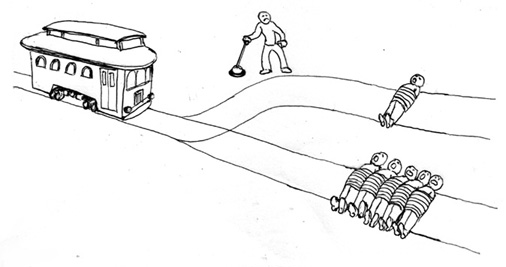
\includegraphics[width=0.7\linewidth]{img/trolley}
	\caption{The Trolley Problem \citep{Foot1967}. Illustration by \href{http://subcortex.com/}{Jesse J. Prinz}.}
	\label{fig:trolley}
\end{figure}

In the first few weeks of my Ph.D., I observed that layman interlocutors, when confronted with this question on the occasion of a social dinner, have a general tendency to conjure up disaster scenarios involving imminent accidents with unavoidable casualties. This reflex is likely to stem from the popularisation of the Trolley Problem \citep{Foot1967}, a famous thought experiment in moral philosophy, depicted in \Cref{fig:trolley}, in which a runaway trolley is headed straight toward five people tied up on the main track and unable to move. When pulled, a lever switches the trolley to a side track occupied by one person: what should you do? Answering this general question of what we \emph{ought} to do in any situation, what is a \emph{right} or \emph{wrong} decision, is the focus of the field of {normative ethics}. This dilemma illustrates a clash between two schools of thought: utilitarianism and deontological ethics. According to utilitarians, the rightfulness of an action should be evaluated based on its consequences, and actions maximising a \emph{utility} --the happiness and well-being for the affected individuals-- should be preferred. Conversely, deontologists evaluate the morality of actions \emph{per se}, according to a series of rules, rather than based on their consequences. Although this problem was initially introduced as a thought experiment, its transposition to the context of autonomous driving and arguably more realistic scenarios made it heavily cited in discussions regarding safety \citep[\eg][]{Lin2015,Bonnefon2016,Gogoll2017}. In early 2017, MIT's Media Lab launched the \emph{Moral Machine} platform \citep{Awad2018}, in which they invited members of the public to select the morally acceptable decision out of several options available to an autonomous vehicle. The authors argued that the recovered global preference would provide \emph{\enquote{essential topics to be considered by policymakers}}, and \citet{Noothigattu2018} proposed an implementation of a system aggregating these preferences, trained on the collected data. However, the relevance of this analogy to inform engineering and policy has been called into question. Thus, \citet{DeFreitas2019} point out that such dilemmas are unlikely to occur on real roads, hard to detect by perception systems and to act upon by control systems, and that they are distracting researchers from the more appropriate goal of how to avoid accidents altogether. Indeed, when we drive, we seldom find ourselves in such extreme situations but rather constantly ponder over less tragic considerations: Where does this vehicle intend to go? Do I have the time to proceed or should I yield? What is the appropriate speed to drive at right now? 
% https://www.grammarphobia.com/blog/2019/08/series-of-questions.html
The object of this thesis is to artificially reproduce this cognitive process of how to avoid accidents while driving, which is more a technical matter than an ethical one. Still, the Trolley Problem, though unrealistic, reveals and raises a number of legitimate questions. Should we base driving decisions on a set of rules? Can these rules be learned, \eg by imitating human drivers? Should we instead make decisions by comparing the utility of possible outcomes, like utilitarians advocate? And if so, how do we choose a good utility? This last interrogation becomes particularly sensitive if we add uncertainty to the Trolley Problem. Facing a potential collision, driving slowly decreases the risk of accident at the expense of efficiency, which can ultimately have an economical impact. What is the \emph{right} level of caution to take? This question directly translates as that of the \emph{value of life}, which has been taken up by economists for decades \citep{Abraham1960,Dreze1962,Schelling1968life,Banzhaf2014,Tirole2017,Charpentier2019} and has countless practical implications for public policies, including recent debates on lowering the speed limits on highways and trunk roads, but also on the appropriate lockdown durations during a pandemic.
It would be illusory to pretend that the practical implications of the Trolley Problem can simply be swept aside and entirely replaced by technicality. Throughout this manuscript, we will see that ethical concerns still underpin most assumptions and design choices of safety-critical software.


\subsection{Nuts and bolts of self-driving software}
\label{sec:nuts-and-bolts}

\begin{figure}[th]
	\centering
	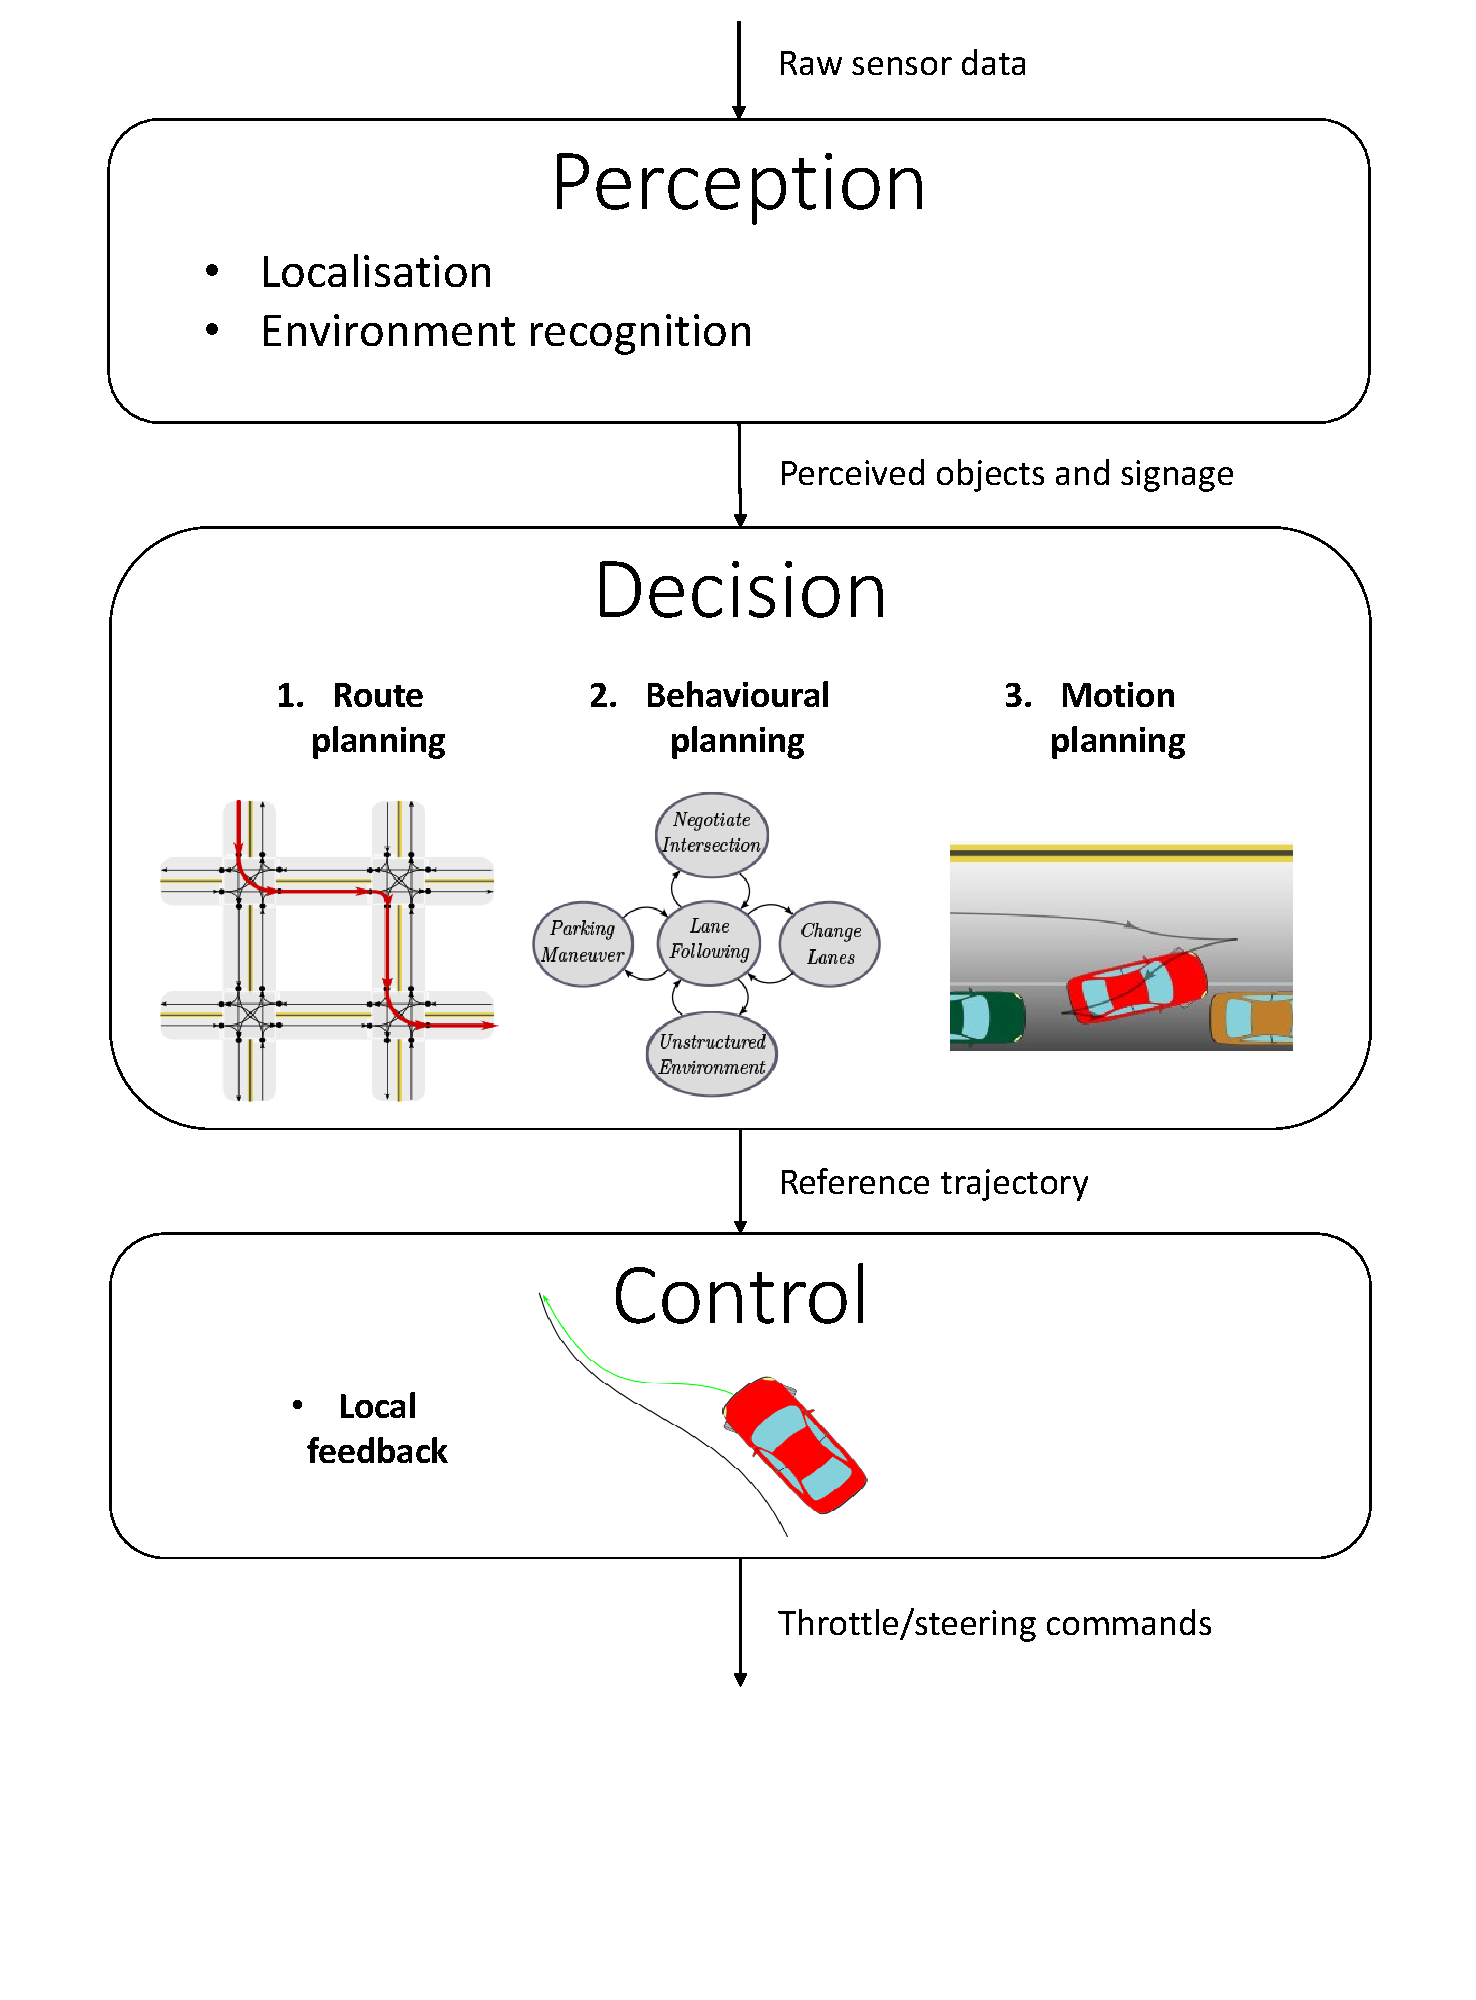
\includegraphics[trim={0 5cm 0 0}, clip, width=0.7\linewidth]{img/pipeline}
	\caption{The architecture of a typical self-driving software}
	\label{fig:robotics-pipeline}
\end{figure}

Historically, autonomous vehicles have been developed following a traditional robotics pipeline, illustrated in \Cref{fig:robotics-pipeline}. This architecture decomposes the task of driving as a series of three functions: \emph{Perception}, \emph{Decision}, and \emph{Control} (also called the Sense-Plan-Act paradigm, or Navigation, Guidance and Control in aerospace engineering). The {Perception} module takes raw sensor data as input and produces a high-level reconstruction of the scene. The {Decision} module then determines the desired trajectory of the vehicle, based on the current situation. Finally, the {Control} module manipulates forces, by way of steering and throttle controls, to track the desired trajectory. In the context of Autonomous Driving, the Decision module is often implemented with a hierarchical structure whose layers work at different timescales. First, a \emph{Route Planning} layer searches for the shortest route in a road network from the current location to the desired destination. Second, the \emph{Behavioural Planning} layer specifies a coarse driving behaviour through short-term goals or semantic decisions, such as changing lane, slowing down at an intersection, or yielding to a vehicle. This layer is thus responsible for following the planned route while adapting to the current state of the traffic in real-time. Third, the \emph{Motion Planning} layer generates a continuous, feasible trajectory that implements the desired behaviour while ensuring comfort and safety.

Great strides have been made in the two end-of-pipe tasks: Perception has benefited from the substantial progress in the field of computer vision due to the recent advent of deep learning \citep[surveyed in][]{janai2017computer}, and many Control schemes \citep[surveyed in][]{Polack2018} have been developed for ground vehicles. In the Decision module, Route Planning is virtually solved and already provided by services such as \href{https://wiki.openstreetmap.org/wiki/Routing}{Open Street Maps}, and there exist a vast body of Motion Planning algorithms, discussed in \Cref{chapter:2}. All these building blocks are widely used for industrial applications, including \gls{ADAS} functions such as \gls{LKA}, \gls{ACC}, \gls{AEB} or \gls{AES}; and in academic research challenges. Ultimately, we claim that Behavioural Planning remains the only neglected link in the chain. Indeed, most of these applications focused so far on simple settings with little complexity: \gls{ADAS} systems are mostly tailored for highway driving and struggle whenever required to interact with other drivers, \eg for merging into traffic\footnote{This difficulty, which motivated this thesis, was reported by engineers from the \gls{ADAS} team at Renault.}.
Similarly, most academic challenges focused on highway driving, with the exception of the DARPA Urban Challenge, which required more advanced interactions with other vehicles. Nevertheless, even this event still constituted a controlled environment, simple enough that all participants could rely on rule-based systems for behavioural planning \citep{Buehler2009}, such as finite state machines whose transitions are triggered by handcrafted criteria \citep[\eg][]{Baker2008}. Unfortunately, there is little hope that this approach can scale to complex scenes since responses tailored for specific use-cases cannot be easily merged. %TODO: ref needed

\subsection{Scope and Challenges of this Thesis}
\label{sec:scopes-and-challenges}

In the light of the above, this thesis is dedicated to addressing a weak link in the \gls{AD} chain: \emph{Behavioural Planning}.  We ask the following question: assuming that we had access to a ground truth perception and a perfectly accurate control system, what steps would remain to achieve fully autonomous driving?


\paragraph{Humans in the loop}

Unless restrained to dedicated infrastructure, Autonomous Vehicles will have to share the road with human drivers. This introduces a great deal of uncertainty in the decision problem. Indeed, while the location and velocity of a vehicle can be perceived, the mind of its driver remains impenetrable. Even though the present state is known, the future becomes uncertain: where are they headed? Are they paying attention to their surroundings? In that regard, it seems impossible to manually model all the factors involved in the human decision-making process. However, human drivers do not drive erratically either, and their behaviour is highly structured: humans drivers tend to follow the lanes, avoid collisions with other vehicles, and generally respect road signage. In other words, human drivers are \emph{predictable}. This motivates the idea of learning from data, and hope for a better comprehensiveness than handcrafted decision systems.%, either direct predictive models of human behaviours or a driving policy based on implicit predictions of what they might do next.
% We want to quantify uncertainty
% Recall aletoric vs epistemic uncertainty?

\paragraph{Learning to act}

The skill of driving a car involves taking a series of decisions, where early stages influence the resulting outcomes and subsequent reasoning at late stages. This aspect is known as sequential (or multistage) decision-making. Let us start by introducing some useful notations. At each time step $t$, the system is described by its \emph{state} $s_t$ that belongs to a measurable\footnote{A measurable space is a set with a $\sigma$-algebra, that allows to define random variables. For example, this set can finite ($[N]$), countable ($\Natural$), or continuous ($\Real$).} state space $\cS$. Then, the agent can take an \emph{action} $a_t$ within a measurable action space $\cA$, before transitioning to a next state $s_{t+1}\in\cS$, drawn from a conditional distribution $\Ps\parentheses{s_{t+1} \mid s_t, a_t}$ that we call the \emph{system dynamics} $\Ps\in\cM(\cS)^{\cS\times\cA}$, where $\cM(\cX)$ denotes the set of probability measures of a measurable set $\cX$. The agent actions can themselves be drawn from a distribution $\policy\parentheses{a_t\mid s_t}$, called the \emph{policy} $\policy\in\cM(\cA)^{\cS}$.

\gls{RL} is a general framework for learning-based sequential decision-making. It is formulated as an optimal control problem: the policy $\policy$ is chosen to maximise an objective function. It is generally formalised as a \gls{MDP}, \ie a tuple $(\gls+{cS}, \gls+{cA}, \gls+{transition}, \R, \discount)$ in which at each step $t$, the agent receives a bounded reward $R(s_t, a_t)$, where $R\in[0, 1]^{\cS\times\cA}$ is a deterministic reward function and $\discount\in[0,1)$ is a discount factor. Adequate long-term behaviour of policies $\policy$ is fostered by considering their \emph{return}.

\begin{definition}[Policy return]
	\begin{leftbar}[defnbar]
	The {return} $\return^{\gls+{policy}}$ of a policy $\policy$ is a random variable defined as the discounted sum of rewards 
	\begin{equation*}
	\gls+{return}^{\gls+{policy}} = \sum_{t=0}^\infty \discount^t \R(s_t, a_t)
	\end{equation*}
	accumulated along a trajectory $\tau = (s_0, a_0, s_1, a_1, \dots)$ induced by the policy $a_t\sim \policy(a_t|s_t)$ and system dynamics $s_{t+1}\sim \Ps(s_{t+1} \mid s_t, a_t)$.
	\end{leftbar}
\end{definition}

The performance of a policy $\policy$ is then evaluated through its \emph{value} function. 
\begin{definition}[Value functions]
	\begin{leftbar}[defnbar]
	\label{def:value-functions}
	The state value $\V^\policy(s)$ of a policy $\policy$ is the expected return of the policy when starting in a state $s$
	\begin{align*}
	\gls+{V}^\policy(s) \eqdef \expectedvalue\left[ \return^\policy \mid s_0=s\right].
	\end{align*}
	Similarly, the state-action value $\Q^\policy(s, a)$ of a policy $\policy$ is the expected return of the policy when starting in the state $s$ and taking the action $a$
	\begin{align*}
	\gls+{Q}^\policy(s, a) &\eqdef \expectedvalue\left[ \return^\policy \mid s_0=s, a_0 = a\right].
	\end{align*}
	\end{leftbar}
\end{definition}

This allows to define the goal of \glsxtrlong{RL}: finding an \emph{optimal} policy $\optimalpolicy$.

\begin{definition}[Optimality]
	\begin{leftbar}[defnbar]
	\label{def:optimality}
	A policy $\gls+{optimalpolicy}$ is said to be optimal if it maximises the value functions $V^\policy$ and $Q^\policy$ in every state and action.
	We also define the optimal value functions $\gls+{V}^\star$ and $\gls+{Q}^\star$ as 
	\begin{align*}
	&\forall s\in \cS, & \gls+{V}^\star(s) &\eqdef Q^{\policy^\star}(s) = \max_\policy V^\policy(s);\\
	&\forall (s,a)\in \cS\times\cA,& \gls+{Q}^\star(s, a) &\eqdef Q^{\policy^\star}(s, a) = \max_\policy Q^\policy(s, a).
	\end{align*}
	\end{leftbar}
\end{definition}

\paragraph{Sample efficiency}
Several performance measures have been introduced to evaluate \gls{RL} algorithms. In this thesis, we consider the goal of finding a near-optimal policy as fast as possible. The \emph{fixed-confidence} setting evaluates the smallest sample complexity, \ie number of interactions, required to find a near-optimal policy $\optimalpolicy$ with high probability. Alternatively, in the \emph{fixed-budget} setting, the \emph{simple regret} $\regret$ of an algorithm measures the \emph{expected} sub-optimality of the recommended policy $\hat{\policy}_n$ after a fixed number $n$ of interactions
\begin{equation*}
\gls+{regret}(s) \eqdef \expectedvalue_{\hat{\policy}_n} \left[ V^\star(s) - V^{\hat{\policy}_n}(s) \right].
\end{equation*}

%Conversely, in real environments where exploration is costly, another objective is to minimise the \textit{cumulative regret}.
%\begin{equation*}
%\cR_n(s_0, \cA) = \expectedvalue_{\hat{\policy}_t\sim \cA}\left[ \sum_{t=0}^{n-1} V^\star(s_t) - V^{\hat{\policy}_t}(s_t) \right]
%\end{equation*}

The goal of this thesis is to provide \emph{sample-efficient} algorithms for learning a driving policy. In the particular context of Behavioural Planning for Autonomous Driving, this goal will be articulated around a few main questions and challenges.

\paragraph{Model-free \vs model-based}

\glsxtrlong{RL} algorithms can be grouped into two main families. 
To find an optimal policy $\optimalpolicy$, model-based \glsxtrlong{RL} algorithms first attempt to estimate the \gls{MDP} parameters $\hat{P}$ and $\hat{R}$ based on a history of transitions $\cD = \{(s_{t},a_t, r_t, s_{t+1})\}$, using for instance \gls{MLE} in a hypothesis class of dynamics and reward functions:
\begin{equation*}
\max_{\hat{P}} \prod_{t}\hat{P}\parentheses{s_{t+1} \mid s_t,a_t} \quad \text{and} \quad \min_{\hat{R}} \sum_{t}\|R(s_t,a_t) - \hat{R}(s_t,a_t)\|^2_2.
\end{equation*}
This allows to \emph{plan} in the estimated \gls{MDP} $(\cS,\cA, \hat{P}, \hat{R}, \discount)$, \ie compute the associated optimal policy $\hat{\policy}^\star$. This can be achieved using planning algorithms such as Dynamic Programming or Linear Programming.
Conversely, model-free \gls{RL} algorithms do not estimate the underlying \gls{MDP} and aim instead to optimise a policy $\policy$ directly. Policy-based methods evaluate the value $Q^\policy$ of the current policy $\policy$, so that it can be locally improved \eg by gradient ascent. Value-based method bypass this alternation of evaluation and improvement steps by directly learning the optimal value function $Q^\star$.

The question of which approach is appropriate depends on the underlying problem. Indeed, model-based techniques are relevant when the dynamics are simple but the optimal policy is complex. For instance, the case of Computer Go was tackled in AlphaGo \citep{Silver2016,Silver2017,Silver2018} with a \gls{MCTS} planning module, which leveraged the knowledge of the Go dynamics (placing pawns on the board) to sample sequences of plies in a game tree. On the contrary, the model-free approach is useful when the system dynamics are complex, but the optimal policy is simple. Thus, a swimming robot would require massive fluid dynamics simulation to accurately predict the effect of moving its fins, while a simple periodic gait could suffice to propel it forward in the water. Which brings us to the question: which scenario does \gls{AD} fall into? Unfortunately, the answer is not so clear-cut. On the one hand, the motion planning literature has historically been heavily relying on kinematics and dynamics models to plan trajectories, as detailed in \Cref{chapter:2}. Reliable priors are available to describe the physics of a vehicle, but not so much for the actual driving policy. On the other hand, automotive companies such as Mobileye reportedly\footnote{These comments are reported from discussions between Renault and Mobileye.} advocated that the task of predicting a driving scene is actually more difficult than that of driving. In fact, the case of \glsxtrlong{AD} is peculiar in that the two problems of prediction and control are somewhat equivalent, due to the presence of other drivers: a good trajectory predictor can be used to predict the action that a human would take in place of the ego-vehicle, and a good driving policy can be applied to each agent in the scene to produce reasonable predictions of their trajectory. Hence, both approaches seem equally relevant and will be considered in this thesis.

\paragraph{Social interactions and coupled dynamics}

To ensure safety while driving, traditional motion planning techniques rely on conservative independence assumptions on the behaviour of other vehicles. This makes them suffer from an effect colloquially known as the \emph{\enquote{freezing robot problem}} \citep{Trautman2010}: due to massive uncertainty, these systems tend to struggle in situations that require interacting --or negotiating-- with other vehicles, such as unprotected left-turns, intersections, or highway merges (see \eg these \href{https://www.youtube.com/watch?v=HjtiiGCe1pE}{two} \href{https://twitter.com/nitguptaa/status/990683818825736192}{videos} where a Waymo car fails to merge). 
Thus, for an autonomous vehicle to efficiently integrate with the traffic flow, it must anticipate the effect of its own actions on the behaviour of other agents. This skill is known as \emph{socially-aware} decision-making. Unfortunately, interactions between vehicles translate into complex and coupled traffic dynamics where local deviations must be propagated from one vehicle to the next, which can result in a quick and chaotic build-up of uncertainty. We will need to contain this escalation to prevent instability in our predictions.

\paragraph{Ensuring safety}

The complexity of the task of driving leads us to consider learning algorithms. However, these methods typically raise a legitimate concern among car manufacturers: how can we guarantee the \emph{safety} of such systems, in the presence of uncertainty? In this thesis, we will strive to formalise this concern by formulating different notions of \emph{risk}, as functions of the distribution of outcomes induced by a policy. We will study \emph{Safe} \glsxtrlong{RL} algorithms, that seek to explicitly estimate and control the level of risk taken by a policy.

\paragraph{Balancing safety and efficiency}
However, protecting against risk often comes at the price of efficiency in achieving a goal.
Consider for a moment a situation where a vehicle is driving slowly in front of you on the road, and so you decide to overtake them. How do you know, at that very moment, that the driver has seen you and is not going to change lane at the last moment, causing an accident? In fact, you don't, at least not with certainty. In this situation, the only way to guarantee safety is to refrain from overtaking. By pushing this simple argument through to its conclusion, it becomes apparent that the only way to \emph{fully} ensure safety is to stay in the garage.
You are thus facing an irreducible dilemma: the two objectives of driving fast and safely are contradictory.
This opposition induces a trade-off that we typically observe with human drivers, especially in situations of negotiations: some people adopt \emph{aggressive} behaviours and try to force their way through traffic, while others act more \emph{defensively}, favouring safety. This ambiguity is difficult to capture manually in an objective function and soon leads to the pitfall of reward engineering. To provide a principled control over this trade-off, the learning algorithms that we consider will be required to respect an \emph{adjustable} level of risk.

\section{Outline and Contributions}

\begin{figure}[ht]
	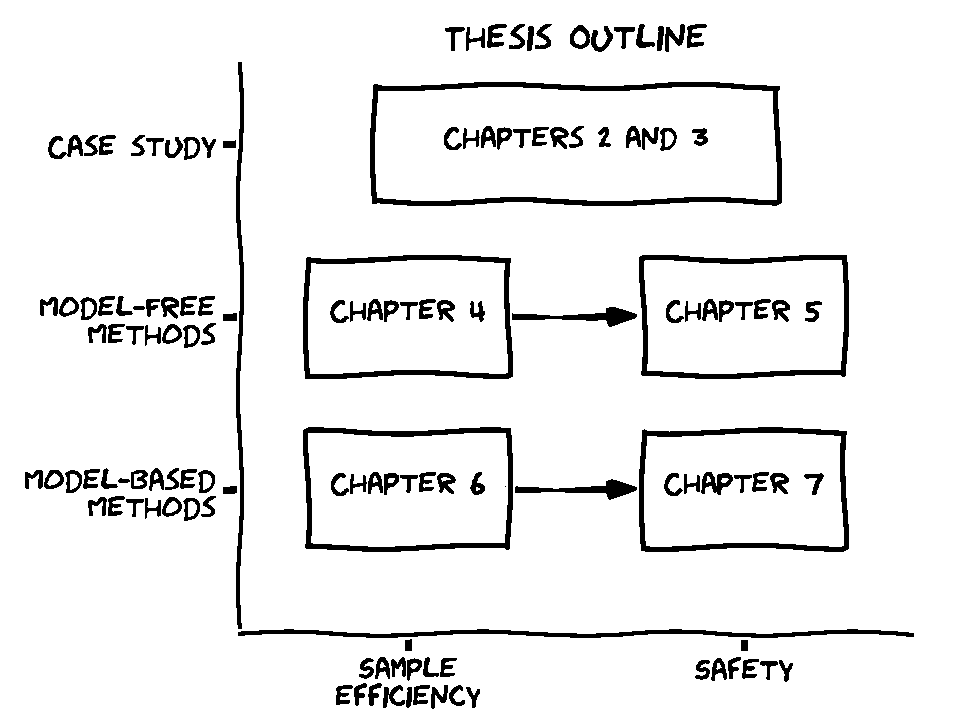
\includegraphics[width=0.9\linewidth]{img/outline}
	\caption{This thesis is structured around two disjunctions: model-free \vs model-based on the one hand, and sample-efficiency \vs safety on the other hand.}
	\label{fig:thesis-outline}
\end{figure}

% Part I
The ultimate goal of this thesis could be summarised in the following question: \emph{\enquote{how can an algorithm learn to drive and avoid accidents?}}. The first step in such an endeavour must necessarily be to formalise more precisely the meaning of this ill-posed formula, which we try to do in \textbf{\Cref{part:1}}.
It is only natural that we begin this effort by turning to the standard model for sequential decision making: the \glsxtrlong{MDP}. At first glance, this framework shines with its simplicity and elegance, but also its apparent generality and representation power. Yet, as we embark on the ambitious task of casting the blurry problem of autonomous driving into this rigid mould, we highlight in \textbf{\Cref{chapter:2}} how reductive each step of the formalisation is, how approximations and assumptions always hide behind each symbol and each equation. This observation is supported by the numerous variations of the framework developed by the research community, in as many attempts to address these concerns. Such limitations are as varied as partial observability, temporal abstraction, the reward hypothesis, transfer from simulation to real-world and safety; and we relate these research directions to specific works in the autonomous driving literature.

In order to progress, we put aside some of these questions in \textbf{\Cref{chapter:3}} and commit to an (observable) state space, a (hierarchical) action space, a (quasi-linear) system dynamics and a (dense) reward function that we deem suitable for a large class of behavioural planning tasks. This allows us to refocus on two fundamental issues: \textit{sample-efficient} and \textit{safe} \glsxtrlong{RL}. In the sequel we tackle them through the perspective of the two main approaches to \glsxtrlong{RL} aforementioned: first model-free, and then model-based algorithms. This organisation is depicted in \Cref{fig:thesis-outline}.

% Part II
\textbf{\Cref{part:2}} is dedicated to the study of how model-free methods can be applied for efficient and safe \glsxtrlong{AD}. In \textbf{\Cref{chapter:4}}, we question the choice of state representation and model architecture in relation to their associated sample-efficiency. In particular, we identify desirable properties and inductive biases that the policy should enjoy, such as \emph{permutation invariance} with respect to vehicles in the scene. We propose an attention-based architecture that fulfils our criteria, and compare it to standard representations and model architectures that have been used for behavioural planning tasks. 

In \textbf{\Cref{chapter:5}}, we consider a continuous notion of risk, defined as an expected discounted sum of a cost signal. This formulation allows highlighting  a trade-off between two separate objectives: the traditional return associated with task completion, and the risk related to safety. In this multi-objective perspective, the Pareto frontier of non-dominated policies defines a spectrum of behaviours, from risk-averse on one side to risk-seeking on the other. In order to explicitly control the level of risk taken in real-time, we place ourselves within the \gls{BMDP} framework, in which the risk is constrained to lie below an --adjustable-- threshold. 
So far, \glspl{BMDP} could only be solved in the case of finite state spaces with known dynamics. This chapter extends the state-of-the-art to environments with continuous state space and unknown dynamics. We show that the solution to a \gls{BMDP} is a fixed point of a novel Budgeted Bellman Optimality operator, which enables to estimate both the expected return and risk of an action, in a model-free fashion. This observation allows us to introduce natural extensions of Deep Reinforcement Learning algorithms to address large-scale \glspl{BMDP}.

% Part III
\textbf{\Cref{part:3}} is devoted to the study of model-based methods, that solve the \glsxtrlong{RL} problem by planning with a learned generative model.
In \textbf{\Cref{chapter:6}}, we assume that a reliable generative model has already been learnt and focus on the sample-efficiency of the planning procedure specifically. More precisely, we look into the theoretical and practical aspects of planning algorithms under budget constraints. First, we consider the \gls{OLOP} algorithm that enjoys good theoretical guarantees but is overly conservative in practice, as we show in numerical experiments. We propose a modified version of the algorithm with tighter upper-confidence bounds, \KLOLOP, that leads to better practical performances while retaining the sample complexity bound. Second, we study a limitation of \gls{MCTS} algorithms: they do not identify together two similar states reached via different trajectories and represented in separate branches of the tree. We propose a \emph{graph-based} planning algorithm, which takes into account this state similarity, provide a regret bound that depends on an improved problem-dependent measure of difficulty, and illustrate its empirical benefits numerically.

In \textbf{\Cref{chapter:7}}, we look back into the issue of \emph{model bias}, which refers to the gap that exists between a learned model and the true system dynamics, and can dramatically degrade the performance of the planned trajectory. More specifically, we study the problem of \emph{robust} and \emph{adaptive} \gls{MPC} of a linear system, with unknown parameters that are learned along the way (adaptive), in a critical setting where failures must be prevented (robust).
To that end, instead of merely considering a point estimate of the dynamics, we leverage non-asymptotic linear regression to build an entire \emph{confidence region} that contains the true dynamics with high probability.
To effectively propagate this parametric uncertainty, we design a predictor that produces a tight interval hull bounding the system trajectories. Having observed the instability of traditional interval predictor techniques, we propose a new one whose stability is guaranteed by a Lyapunov function analysis and verification of linear matrix inequalities.
These tools enable us to guarantee the system stabilisation and robust constraint satisfaction, through an \gls{MPC} algorithm based on a stabilising control that uses the predicted interval.
Finally, in order to go beyond stabilisation problems only, we tackle the minimax control of more general (non-convex) costs that naturally arise in many practical problems. To that end, we combine our results with the tree-based planning techniques of \Cref{chapter:6}. By adapting the theoretical guarantees at each layer, we provide the first end-to-end regret analysis for this setting. Interestingly, our analysis naturally adapts to handle multiple models and combines with a data-driven robust model selection strategy, which enables to relax the modelling assumptions. We strive to preserve tractability at any stage of the method, that we illustrate numerically.

%!TEX root = ../PhD_thesis__Edouard_Leurent

\subsection*{List of publications}

\subsubsection*{Publications in international conferences with proceedings}

\begin{itemize}
	\item \fullcite{Leurent2020beyond} (used in \Cref{chapter:7})
	\item \fullcite{Leurent2020monte} (used in \Cref{chapter:6})
	\item \fullcite{Leurent2020robust} (used in \Cref{chapter:7})
	\item \fullcite{CarraraLeurent2019} (used in \Cref{chapter:5})
	\item \fullcite{Leurent2019interval} (used in \Cref{chapter:7})
	\item \fullcite{Leurent2020practical} (used in \Cref{chapter:6})
\end{itemize}

\subsubsection*{Workshop presentations in international conferences}

\begin{itemize}
	\item \fullcite{Leurent2019social} (used in \Cref{chapter:4})
	\item \fullcite{Leurent2018approximate} (used in \Cref{chapter:7})
\end{itemize}

\subsubsection*{Software}

\begin{itemize}
	\item \fullcite{highway-env} (used in \Cref{chapter:3,chapter:4,chapter:5,chapter:6,chapter:7})
\end{itemize}

\subsubsection*{Collaborations not presented in this thesis}

\begin{itemize}
	\item \fullcite{Menard2020Fast}
	\item \fullcite{Kaufmann2020adaptive}
	\item \fullcite{Jonsson2020planning}
\end{itemize}

\part[Case Study: Learning to Drive]{Case Study:\\Learning to Drive}
\label{part:1}

%!TEX root = ../../PhD_thesis__Edouard_Leurent

\graphicspath{{2-Chapters/2-Chapter/}}

\chapter{Literature Review}
\label{chapter:2}

\begin{flushright}
	\begin{tabular}{@{}l@{}}
		\emph{Souhaite que la route soit longue. [\dots]}\\
		\emph{Visite aussi beaucoup de villes égyptiennes,}\\
		\emph{et n’aie de cesse de t’instruire auprès de ceux qui savent.}\\
	\end{tabular}
	
	Konstantinos Kavafis, \href{https://eleurent.github.io/sisyphe/texts/ithaki.html}{\emph{Ithaque}}.
\end{flushright}

\section{Sequential decision-making}
\label{sec:sequential-decision-making}

The skill of driving a car involves taking a series of decisions, where early stages influence the resulting outcomes and subsequent reasoning at late stages. This aspect is known as sequential (or multistage) decision-making. Let us start by introducing some useful notations. At each time step $t$, the system is described by its \emph{state} $s_t$ that belongs to a measurable state space $\cS$. Then, the agent can take an \emph{action} $a_t$ within a measurable action space $\cA$, before transitioning to a next state $s_{t+1}\in\cS$, drawn from a conditional distribution $P\parentheses{s_{t+1} \mid s_t, a_t}$ that we call the \emph{system dynamics}. The agent actions can themselves be drawn from a distribution $\pi\parentheses{a_t\mid s_t}$, called the \emph{policy}. This section describes the main design principles for coming up with a good driving policy $\pi$.

\subsection{Motion Planning}

The development of motion planning techniques for intelligent vehicles date back to the late 80s, supported by international research projects such as Eureka (1987) of the Prometheus program, followed by the DARPA Grand and Urban Challenges (2004, 2007), and more recently the VIAC (2010), GCDC (2011) and Delphi (2015) challenges. In two surveys \citep{Gonzalez2016,Paden2016} studying the literature of this period, three main approaches have been identified.

\paragraph{Search-based algorithms}

This method is based on a regular discrete partition of the state space $\cS$ called a \emph{lattice}, which must be connected by feasible state transitions \citep[\eg][]{Pivtoraiko2005}. This framing reduces motion planning to the problem of finding a shortest path in a known graph. Then, traditional graph-search algorithms such as Dijkstra's algorithm \citep{Dijkstra1959}, $A^\star$ \citep{Hart1968} or $D^\star$ \citep{Stentz1994} can been used to compute the optimal trajectory. This technique has been applied by at least five different teams during the DARPA Urban Challenge for driving on structured roads and unstructured parking: Dijkstra for team Ben Franklin \citep{Bohren2008} and VictorTango \citep{Bacha2008}, and $A^\star$ for Stanford University \citep{Montemerlo2008} and KIT \citep{Kammel2008}, and $D^\star$ by the winning team from CMU \citep{Urmson2008}.

\begin{figure}[tp]
	\centering
	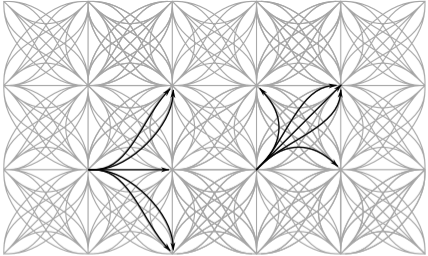
\includegraphics[width=0.5\linewidth]{img/lattice2}
	\caption{TODO: lattice}
\end{figure}

\paragraph{Sampling-based algorithms}

The limitation of search-based algorithms lies in the difficulty of formulating a regular lattice structure which feasible transitions between configurations, and in the real-time constraint that may not be met by graph-search algorithms. To address them, sampling-based motion planners iteratively grow a set of reachable configurations by randomly sampling valid transitions. The most popular ones are Probabilistic Roadmap (PRM) \citep{Kavraki1996}, Rapidly-exploring Random Trees (RRT) \citep{Lavalle98,Karaman2011} and Monte-Carlo Tree Search algorithms \citep[e.g.][]{Kocsis2006}.
\TODO{these methods are used in the context of AD in...}

\paragraph{Optimisation-based algorithms}

The third approach consists in directly optimizing a parametrized trajectory. An example is interpolation between the current and goal states, which has been applied to various classes of functions in the context of Autonomous Driving, such as lines and circles \citep{Reeds1990}, clothoids \citep{Funke2012}, polynomials \citep{Xu2012}, and Bézier curves \citep{Gonzalez}.

Motion planning techniques thus rely on deterministic models of the vehicle dynamics. These models are often required to take a simple form so that the search or optimisation procedure can be solved efficiently. Therefore, other objects are considered static and complex behaviours such as interactions between vehicles are left-out.
\TODO{collaborative planning, centralized (joint behaviour is optimised): does not allow human drivers, uncertainty. example ref: https://ieeexplore.ieee.org/document/736775}
Consequently, these techniques have mainly been successfully applied to the control of a single vehicle to track a sequence of known waypoints with static obstacles.

\subsection{Imitation Learning}

An orthogonal strategy to motion planning techniques is to learn a reactive policy $\pi(a|s)$ under supervision of an expert $\pi_E$ that produces a dataset $\cD$ of demonstration trajectories. To that end, a parametrized policy $\pi_\theta$ is optimised to minimise a regression loss $\cL$, for instance the $KL$ divergence to the expert actions distribution:
\begin{equation*}
\min_\theta \expectedvalue_{s\sim \cD} \left[\cL\left(\pi_{\theta}(a|s), \pi_E(a|s)\right)\right]
\end{equation*}

This approach is particularly suited when only low-level high-dimensional inputs are available, such as camera images, which prevents access to the dynamics model required by motion planning approaches. 
The first application of imitation learning to autonomous driving is the ALVINN (Autonomous Land Vehicle In a Neural Network) project \citep{Pomerleau89}, where a 3-layer neural network was trained for the task of road following, as shown in \Cref{fig:alvinn}.

\begin{figure}[tp]
	\centering
	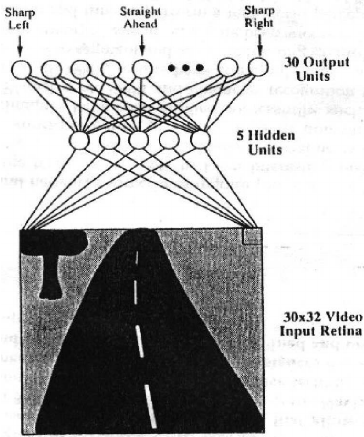
\includegraphics[width=0.4\linewidth]{img/alvinn}
	\caption{The 3-layer architecture used in ALVINN \citep{Pomerleau89}.}
	\label{fig:alvinn}
\end{figure}

\TODO{Compounding errors: \emph{"Supervised learning will not produce a policy with good long-horizon
performance, since a small mistake on the part of the policy will place the system
into states that are outside the distribution in the training data"} \citep{Levine2016}}
\TODO{ref needed: Dagger.}

\begin{figure}[tp]
	\centering
	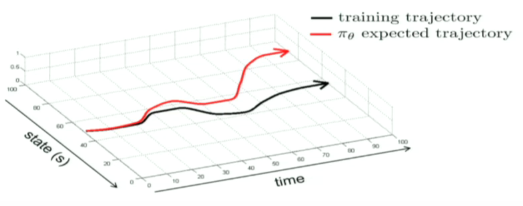
\includegraphics[width=0.7\linewidth]{img/cp4}
	\caption{TODO: Compounding errors}
\end{figure}

To mitigate this issue, \citep{Bojarski2016} proposed to simulate deviations from the expert trajectories using side cameras. The corresponding expert action labels were obtained by adding a constant steering wheel angle to adjust.

\citep{Eraqi2017,Xu2017} proposed to consider temporal dependencies by using recurrent neural networks.

\citep{Kuefler2017,Bhattacharyya2018} used Generative Adversarial Networks to...

But simply imitating is not enough, we need to control the agent / condition the policy with a goal. \citep{Codevilla2018}

\subsection{Reinforcement Learning}

Reinforcement Learning is a general decision-making framework formulated as an optimal control problem. It is typically formalized as a \emph{Markov Decision Process} (MDP), in which at each time step $t$, an agent observes its current state $s_t\in S$ and picks an action $a_t\in A$, before transitioning to a next state $s_{t+1}\in S$ drawn from a transition distribution $P(s_{t+1}|s_t,a_t)$ and receiving a bounded reward $r_t\in[0, 1]$ drawn from a reward distribution $P(r_t|s_t,a_t)$. The agent must act so as to optimise in expectation its cumulative discounted reward, also called \emph{return}, where $\gamma\in[0,1)$ is the discount factor:

\begin{equation*}
\max_{\pi}\expectedvalue_{\pi, P} \left[\sum_t \gamma^t r_t\right].
\end{equation*}

Convenient framework for analysis, but it's often too narrow a frame for the real world to fit in. In the following, we will enumerate several assumptions behind the MDP framework that may not hold in practice, and for which variants have been developed. We will focus on applications of the variants the particular context of Autonomous Driving.

\section{States and partial observability}

The first modelling assumption of the MDP framework is that the agent perfectly knows its own state $s\in\cS$. In practice, information about the scene can only be obtained through sensors, which produce typically noisy measurements. In addition to noise, some part of the state may simply be missing: occlusion.
\TODO{Insert image of partial observability}

Proposed model: POMDP.
Belief state propagation: Kalman filtering for linear system and gaussian noise.
Algo: PBVI, POMCP

Examples:
- Sensor noise: [Probabilistic Online POMDP Decision Making for Lane Changes in Fully Automated Driving]
- Motion planning for a UAV with no GPS, landmark localization: [A POMDP Approach to Robot Motion Planning under Uncertainty]. 
- Planning at an intersection with a moving occluded obstacle (8D system): [Solving Continuous POMDPs:  Value Iteration with Incremental Learning of an Efficient Space Representation]
- ?? : [Probabilistic decision-making under uncertainty for autonomous driving using continuous POMDPs]
- The other drivers locations are observed but not their intentions [Intention-Aware Motion Planning]. MOMDP framework.
- [ Probabilistic Decision-Making at Road Intersections: Formulation and Quantitative Evaluation ]
- Kalman + POMCP for intersection [https://arxiv.org/abs/1704.04322]
- Sunberg: evaluate the POMDP vs MDP approximation with an assumed internal state.
 

\section{Actions and temporal abstraction}
\section{Rewards and inverse reinforcement learning}
\section{Dynamics and transfer}
\section{Optimisation criterion and safety}

%!TEX root = ../../PhD_thesis__Edouard_Leurent.tex

\graphicspath{{2-Chapters/3-Chapter/}}

% Il est un jour, une heure, où dans le chemin rude,
% Courbé sous le fardeau des ans multipliés,
% L'Esprit humain s'arrête, et, pris de lassitude,
% Se retourne pensif vers les jours oubliés.
% Charles-Marie LECONTE DE LISLE - Dies Irae

At the violet hour, when the eyes and back
Turn upward from the desk, when the human engine waits
Like a taxi throbbing waiting,
I Tiresias, though blind, throbbing between two lives,
Perceived the scene, and foretold the rest —

\chapter{Problem Statement}
\label{chapter:3}


\abstractStartChapter{}%
Having discussed at length the range of \glsxtrlong[hyper=false]{AD} modelling perspectives in \Cref{chapter:2}, we now formalize the specific problem that we are going to consider in this thesis. This chapter attempts to cast Behavioural Planning as a \glsxtrlong{MDP}, by specifying each element of a $(\cS, \cA, \Ps, \R, \discount)$ tuple suitable for a set of tactical decision-making tasks.
\minitocStartChapter{}

\section{Perceived states}

As discussed in \Cref{sec:nuts-and-bolts,sec:partial-observability}, information about the world is typically obtained from noisy sensory measurements. The Perception module is responsible for recognizing and tracking the signal from the noise, so as to provide a high-level probabilistic description of the scene. In particular, 
\begin{enumerate}[label=(\roman*)]
	\item a \emph{Mapping} layer reconstructs the geometry of the road network and its associated signage, including stop signs and traffic lights;
	\item a \emph{Localisation} layer recovers the position, velocity and heading of the ego-vehicle;
	\item a \emph{Scene understanding} layer returns the position, velocity and geometry of any vehicle or obstacle nearby.
\end{enumerate}

Since we focus on the Decision module, we will take a simplifying assumption and ignore all aspects related to Perception.
Namely, we take the liberty of assuming to a noise-free access to every feature of the driving scene that we will deem relevant.

\paragraph{Vehicles}

As mentioned in \Cref{chapter:1}, the main challenge of Behavioural Planning is to interact with other vehicles. Therefore, the state should include a description of every vehicle nearby. In addition to the ego-vehicle, indexed by 0, the scene contains a number $N_v$ of other vehicles indexed by the range $[1, N_v]$.
Any vehicle of index $i\in[0,N_v]$ is represented by 
\begin{enumerate}[label=(\roman*)]
	\item its position $(x_i, y_i)\in\Real^2$,
	\item its forward speed $v_i\in\Real$, 
	\item its heading $\psi_i\in\Real$.
\end{enumerate}

The resulting joint state is the traffic description: 
$$s = \begin{bmatrix}
x_0 & y_0 & v_0 & \psi_0\\
\vdots & \vdots & \vdots & \vdots\\
x_{N_v} & y_{N_v} & v_{N_v} & \psi_{N_v}\\
\end{bmatrix}
\in\cS \eqdef\Real^{(N_v+1) \times 4}.$$

We can make a few observations: first, the state space is continuous, which means we will have to resort to function approximation to represent either the policy $\pi$, the value function $Q$ or the dynamics $P$. Second, it has a variable size, since it depends on the number of vehicles nearby, which the function approximation scheme will have to accommodate. Its dimensionality should be in the order of fifty at most, for a dozen observed vehicles.

\paragraph{Roads}

We also assume knowledge of the road network, comprising:
\begin{enumerate}[label=(\roman*)]
	\item a graph description of the network topology, where the nodes represent intersections and the edges represent road segments;
	\item the geometry of every lane $L$ in the network (every edge), described by its centre-line parametric curve
	$
	s \rightarrow (x_{L}(s), y_{L}(s))\in \Real^2,
	$
	\noindent and heading $\psi_L:s \rightarrow \tan^{-1}\left({\odv{y_L}{s}(s)}/{\odv{x_L}{s}(s)}\right) \in \Real$
	where $s\in[0, l_L]$ is the curvilinear abscissa and $l_L$ is the length of the lane $L$.
\end{enumerate}

However, we do not include these information as part of the state but rather of the system dynamics, described later. Consequently, model-free algorithms will learn policies tailored for the particular scene seen during training, and will not be able to adapt to different scenes, unless the state space is augmented to include road features. Conversely, model-based algorithms can leverage road information in their dynamics models and thus generalize to unseen scenes.

\section{Behavioural decisions}

We follow the hierarchical architecture of the Decision module discussed in \Cref{sec:nuts-and-bolts,sec:temporal-abstraction}. Since we focus on Behavioural Planning specifically, we assume the availability\footnote{These two modules are described as part of the dynamics.} of
\begin{enumerate}[label=(\roman*)]
	\item a Route Planning layer, that automatically selects the next road segment to be followed at each intersection, \eg the proper exit on a highway, or the right direction at an intersection;
	\item a Motion Planning and Control layer, that controls the vehicle by way of low-level throttle and steering actuators to reach any desired position and speed in the selected road segment. 
\end{enumerate}

Thus, the purpose of the Behavioural Planning layer is to specify short-term instructions for the Motion Planning layer, in the form of a lane to follow and a speed to adapt. The produced trajectory will always conform to the planned route, but the Behavioural Planner is in charge of \eg deciding when to merge on a highway, negotiating right of way at an intersection, overtaking vehicles, \etc. To that end, we specify the following space of \emph{meta-actions}:

\[
\cA \eqdef \left\{ \begin{array}{c}
\text{change to the left lane},\, \text{change to the right lane}, \\
\text{drive faster},\, \text{drive slower},\, \text{maintain speed and lane}
\end{array}\right\}
\]

Meta-actions are executed at a frequency of $\SI{1}{\hertz}$. Their influence on the evolution of the state $s\in\cS$ is described next.

\section{Traffic dynamics}

This section describes how the behavioural decisions influence the evolution of the perceived states, under their above definitions, through the dynamics distribution $P\parentheses{s' \mid s,a}$. As explained in \Cref{chapter:1}, it is crucial that the simulated vehicles in the scene are able to \emph{react} to the actions of the ego-vehicle, so that interaction patterns can be learnt.

\subsection{Kinematics}

We represent the non-holonomic motion capabilities of every vehicle $i\in[0, N_v]$ in the scene by the Kinematic Bicycle Model \citep[see \eg][]{Polack2017}:
\begin{align}
\begin{split}
\dot{x}_i &= v_i\cos(\psi_i + \beta_i), \\
\dot{y}_i &= v_i\sin(\psi_i + \beta_i),\\
\dot{v}_i &= a_i,\\
\dot{\psi}_i &= \frac{v_i}{l}\sin(\beta_i),
\end{split}
\end{align}
where $l$ is the vehicle half-length, $a_i$ is the throttle command and $\beta_i$ is the slip angle at the centre of gravity, used as a steering command.

\subsection{Motion planning and control}

We equip the ego-vehicle --and also other vehicles $i\in[0, N_v]$ in the scene-- with a capability to execute the meta actions $\cA$. This requires the ability to follow a lane $L_i$, described by the road information mentioned above through its lateral position $y_{L_i}$ and heading $\psi_{L_i}$ . To that end, vehicles follow a cascade controller of lateral position and heading in the form
\begin{align}
\label{eq:heading-command}
\begin{split}
\dot{\psi}_i &= K_i^\psi\left(\psi_{L_i}+\sin^{-1}\left(\frac{\tilde{v}_{i,y}}{v_i}\right)-\psi_i\right),\\
\tilde{v}_{i,y} &= K_i^y (y_{L_i}-y_i),
\end{split}
\end{align}
where $K_i^y\in\Real$ and $K_i^\psi\in\Real$ are control gains.
Note that the corresponding steering command $\beta_i$ can be obtained from \eqref{eq:heading-command} as: $$\beta_i = \sin^{-1}\left(\frac{l}{v_i}\dot{\psi}_i\right).$$

Furthermore, the ego-vehicle needs to be able to control its speed as per the meta actions $\cA$. To that end, we use a linear longitudinal controller
\begin{equation*}
a_0 = K_0^v(v_r - v_0),
\end{equation*}
where $v_r\in\Real$ is the reference speed, incremented by $\pm \SI[per-mode=symbol]{5}{\meter\per\second}$ by the \emph{drive faster} and \emph{drive slower} meta-actions, and $K_0^v\in\Real$ is a control gain.

\subsection{Behavioural models}

Other simulated vehicles follow simple and behavioural models from the traffic simulation literature, that dictate how they accelerate and steer on the road.

\paragraph{Longitudinal behaviour}

The acceleration command $a_i$ of a vehicle $i\in[1, N_v]$ is controlled directly by the \gls{IDM} from \citep{Treiber2000}:
\begin{align}
\begin{split}
a_i &= a\left[1-\left(\frac{v}{v_0}\right)^\delta - \left(\frac{d^{\star}_i}{d_i}\right)^2\right], \\
\text{where }\quad d^{\star}_i &= d_0 + Tv_i + \frac{v_i\Delta v_i}{2\sqrt{ab}},
\end{split}
\end{align}
$v_i$ is the vehicle velocity, $d_i$ is the distance to its front vehicle.
The dynamics are parametrised by the desired velocity $v_0$ , the time gap $T$, the jam distance $d_0$, the maximum acceleration $a$ and deceleration $b$, and the velocity exponent $\delta$.

\paragraph{Lateral behaviour}

The discrete lane change decisions are given by the \gls{MOBIL} model from \citep{Kesting2007}.
According to this model, a vehicle $i\in[1, N_v]$ decides to change lane when

\begin{enumerate}[label=(\roman*)]
	\item it is \emph{safe} to cut-in:
		\begin{equation*}
			\tilde{a}_n \geq - b_\text{safe};
		\end{equation*}
	\item there is an \emph{incentive}, for the ego-vehicle and possibly its followers:
		\begin{equation*}
		\underbrace{\tilde{a}_c - a_c}_{\text{the vehicle}} + p\left(\underbrace{\tilde{a}_n - a_n}_{\text{new follower}} + \underbrace{\tilde{a}_o - a_o}_{\text{old follower}}\right) \geq \Delta a_\text{th};
		\end{equation*}
\end{enumerate}
where $c$ is the centre vehicle, $o$ is its old follower \emph{before} the lane change, and $n$ is its new follower \emph{after} the lane change; $a$ and $\tilde{a}$ are the predicted accelerations of the vehicles \emph{before} and \emph{after} the lane change respectively; $p$ is a politeness coefficient, $\Delta a_\text{th}$ is the acceleration gain required to trigger a lane change; and $b_\text{safe}$ is the maximum braking imposed to a vehicle during a cut-in.

A lane change decision modifies the target lane $L_i$ followed by vehicle $i$ on its current road segment. The actual trajectory planning and steering control to track this lane is then performed by the lateral controller of \eqref{eq:heading-command}.

\subsection{Route planning}

So far, we explained how both the ego-vehicle ($i=0$) and the other simulated vehicles ($i\in[1, N_v]$) behave on a multi-lanes road segment, through their Behavioural and Control layers. The Route Planning layer is finally responsible for selecting the sequence of road segments leading to a destination, sampled randomly at initialisation. To that end, the Route Planning performs a Breadth First Search in the graph description of the road network mentioned above, and returns a shortest path of road segments from initial position to destination.

In the end, we make the decision of framing the state space $\cS$ as fully observable but subjected to uncertain transition dynamics $P\parentheses{s' \mid s, a}$, which are parametrised by several unobserved variables including the destinations of agents in the scenes and the parameters of their Behavioural and Control layers.

\section{Rewards}

As discussed in \Cref{sec:irl}, choosing an appropriate reward function that yields realistic optimal driving behaviour is a challenging problem, that we do not address in this thesis. In particular, we do not wish to specify every single aspect of the expected driving behaviour inside the reward function, such as keeping a safe distance to the front vehicle. Instead, we would rather only specify a reward function as simple and straightforward as possible, and focus solely on the difficulties related to safe decision-making under uncertainty, in the hope to see adequate behaviour emerge from learning. In this perspective, keeping a safe distance would be optimal not for being directly rewarded but for robustness against the uncertain behaviour of the leading vehicle, which could brake at any time.

Thus, we focus on only two features: a vehicle should
\begin{enumerate*}[label=(\roman*)]
	\item progress quickly on the road;
	\item avoid collisions.
\end{enumerate*}

Since the Markov Decision Process formalism requires rewards to be bounded, by convention we normalize them in the $[0, 1]$ range.
Note that we forbid negative rewards, since they may incentivise the agent to prefer terminating an episode early (by causing a collision) rather than risking suffering a negative return if no satisfying trajectory can be found.

Thus, unless otherwise stated, the reward function $R$ is chosen as follows:
\[
R(x) = 
\begin{cases}
1 & \text{if the ego-vehicle is at full speed;}\\
0 & \text{if the ego-vehicle has collided with another vehicle;}\\
0.5 & \text{else.}
\end{cases}\]

A more realistic reward function may include comfort terms, such as penalizing high acceleration or jerk, and lane changes manoeuvres, but we do not consider them for simplicity.

This reward function is \emph{dense}, since the maximum reward can easily be obtained from any state by accelerating, which should guide exploration to efficient driving styles. However, it is also \emph{non-convex}, since \eg the collision penalty is incurred at the locations of any two obstacles but not in-between. It is even \emph{non-smooth}, given that it its discontinuous at collision states.

\section{Implementation}

\begin{figure}[ht]
	\centering
	
\includegraphics[width=0.6\linewidth]{img/he-git}\\
	
\includegraphics[height=0.5cm]{img/he-buil.pdf}
	
\includegraphics[height=0.5cm]{img/he-docs.pdf}
	
\includegraphics[height=0.5cm]{img/he-qual.pdf}
	
\includegraphics[height=0.5cm]{img/he-cov.pdf}
	
\includegraphics[height=0.5cm]{img/he-contr.pdf}
	
\includegraphics[height=0.5cm]{img/he-envs.pdf}
	\caption{\textsc{highway-env} repository status (on 30/06/2020).}
	\label{fig:highway-env-status}
\end{figure}

I created the \href{https://github.com/eleurent/highway-env}{\textsc{highway-env}} environment: a minimalist driving simulator tailored for behavioural planning tasks, following the \gls{MDP} formalization presented in this chapter. It is written in Python and published online under an open-source license \citep{highway-env}. An extensive documentation is also available, along with instructions to reproduce every numerical experiments presented throughout this manuscript. We discuss at length the features and architecture of this project in \Cref{chapter:a}. We mention that in addition to our own works, several students and researchers already make use of this environment, as shown in \Cref{fig:highway-env-status}.



\part{Model-free}
\label{part:2}

\vspace*{2cm}
\begin{flushright}
	\begin{tabular}{@{}l@{}}
		\emph{Agir en primitif\dots}\\
	\end{tabular}
	
	René Char, \href{https://eleurent.github.io/sisyphe/texts/feuillets-d-hypnos.html}{\emph{Feuillets d'Hynos}}.
\end{flushright}

%!TEX root = ../../PhD_thesis__Edouard_Leurent.tex

\graphicspath{{2-Chapters/4-Chapter/}}

\tikzset{
	state/.style={
		rectangle,
		draw=black, very thick,
		minimum height=2em,
		inner sep=2pt,
		text centered,
	},
	name plot/.style={every path/.style={name path global=#1}}
}

\chapter{Considering Social Interactions}
\label{chapter:4}

\begin{flushright}
	\begin{tabular}{@{}l@{}}
		\emph{O what a strange parcel of creatures are we,}\\
		\emph{Scarce ever to quarrel, or even agree;}\\
		\hdashline
		\emph{Like social companions we never fall out,}\\
		\emph{Nor ever care what one another’s about;}\\
	\end{tabular}
	
	Elizabeth Hands, \href{https://eleurent.github.io/sisyphe/texts/unsociable_family.html}{\emph{On An Unsociable Family}}.
\end{flushright}

\abstractStartChapter{}%
Having detailed the \gls{MDP} model in \Cref{part:1}, we now study in \Cref{part:2} how model-free \glsxtrlong{RL} algorithms can learn an optimal behavioural planning policy. In this chapter, we focus on the design of \emph{sample-efficient} learning architectures, tailored for dense traffic situations. Such architectures should deal with a varying number of nearby vehicles, be invariant to the ordering chosen to describe them, while staying accurate and compact. We observe that the two most popular representations in the literature do not fit these criteria, and perform badly on an complex negotiation task. We propose an attention-based architecture that satisfies all these properties and explicitly accounts for interactions between the traffic participants. We empirically show that this architecture enjoys significant performance gains, and is able to capture interactions patterns that can be visualised and qualitatively interpreted.\footnote{This chapter is based on a preprint \citep{Leurent2019social} presented at the \emph{Machine Learning for Autonomous Driving workshop} at the NeurIPS 2019 conference. It is a collaboration with my friend and colleague Jean Mercat, who pursued this idea in further work on trajectory forecasting, which was published at the \emph{2020 International Conference on Robotics and Automation} \citep{Mercat2020} and won two international competitions.}
\minitocStartChapter{}

\section{Motivation}

Value-based \glsxtrlong{RL} algorithms such as Q-Learning \citep{Watkins1992} and its variants rely on estimating the optimal state-action value function $\Q^\star$. Since the state space $\cS$ chosen in \Cref{chapter:3} is continuous, we must resort to function approximation. Thus, independently of how $\cS$ was defined, we now have to specify how a state $s\in\cS$ will be \textit{represented} as an input to parametrised model $\gls+{Q}_\params$. The choice of both the model class and state representation will strongly influence the system performances. In particular, we claim that the two most-widely used representations both suffer from different drawbacks: on the one hand, the \emph{list of features} representation is compact and accurate but has a varying-size and depends on the choice of ordering. On the other hand, the \emph{spatial grid} representation addresses these concerns but in return suffers from an accuracy-size trade-off.

Our contributions are the following: first, we propose an attention-based architecture for decision-making involving social interactions. This architecture allows to satisfy the variable-size and permutation invariance requirements even when using a \emph{list of features} representation. It also naturally accounts for interactions between the ego-vehicle and any other traffic participant.
Second, we evaluate our model on a challenging intersection-crossing task involving up to 15 vehicles perceived simultaneously. We show that our proposed method provides significant quantitative improvements, and that it enables to capture interaction patterns in a way that is visually interpretable.

\section{Background}

\label{sec:background}

We start by giving some background on standard model-free learning algorithms --with a focus on value-based methods--, on usual state representations used for behavioural planning, and on attention mechanisms for \glspl{NN}.

\subsection{Value-based deep \glsxtrlong{RL}}

Recall from \Cref{def:optimality} that $Q^\star$ can be computed from an optimal policy $\optimalpolicy$ since $\Q^\star = \Q^{\optimalpolicy}$. However, the converse that $\optimalpolicy$ can be obtained from knowing $\Q^\star$ is also true since
\begin{proposition}[Optimality of the greedy policy, \citealp{Bellman1957}]
	\begin{leftbar}[propositionbar]
	A greedy policy defined as
	\begin{equation*}
	\forall s\in\cS, \optimalpolicy\parentheses{\cdot \mid s} = \dirac_{a^\star},\,\text{where } {a^\star}\in \argmax_a \Q^\star(s, a),
	\end{equation*}
	and $\dirac_x = \dirac(x-\cdot)$ denotes the Dirac distribution in $x$, is optimal.
	\end{leftbar}
\end{proposition}

Finding an optimal policy thus reduces to computing the optimal value function $Q^\star$. Fortunately,
\begin{theorem}[Bellman Optimality Equation, \citealp{Bellman1957}]
\label{thm:bellman-optimality-mdp}
\begin{leftbar}[theorembar]
The optimal action-value function $Q^\star$ satisfies the Bellman Optimality Equation:
\begin{equation*}
\Q^\star(s, a) = (\bo \Q^{\star}) (s, a) \eqdef \expectedvalueover{s'\sim \Ps(s'|s, a)} \max_{a'\in \cA} \left[\R(s, a) + \discount \Q^\star(s', a')\right].
\end{equation*}
Moreover, $\bo$ is a $\discount$-contraction for the $\|\cdot\|_\infty$ norm:
\begin{equation*}
\forall Q_1, \Q_2\in \Real^{\cS\times\cA},\; \|\bo Q_1 - \bo Q_2\|_\infty \leq \gamma \|Q_1 - Q_2\|_\infty.
\end{equation*}
\end{leftbar}
\end{theorem}

Thus, since $Q^{\star}$ is a fixed-point of a contracting operator, it can be computed by iteratively applying $\bo$ in a fixed-point iteration fashion. The \emph{Q-learning} algorithm \citep{Watkins1992} follows this procedure by applying a sampling version $\bo$ to a batch of collected experience. When dealing with a continuous state space $S$, we need to employ function approximation in order to generalise to nearby states. The  \gls{DQN} algorithm \citep{Mnih2015humanlevel} implements this idea by using a neural network model to represent the action-value function $Q$.

\subsection{Common traffic state representations}

In order to apply a reinforcement learning algorithm such as \gls{DQN} to an autonomous driving problem, a state space $S$ must first be chosen, that is, a representation of the scene. The state should at least contain a description of every nearby vehicle, when social interactions are relevant to the decision. We recall our definition \eqref{eq:state-space} of $\cS$ from \Cref{chapter:3}, in which a vehicle driving on a road is described by it's continuous position, heading and velocity, and the joint state of a road traffic with one ego-vehicle denoted $s_0$ and $N_v$ other vehicles can be described by a list of individual vehicle states:
\begin{equation*}
s = \begin{bmatrix}
p^x_0 & p^y_0 & v_0 & \psi_0\\
\vdots & \vdots & \vdots & \vdots\\
p^x_{N_v} & p^y_{N_v} & v_{N_v} & \psi_{N_v}\\
\end{bmatrix}
\in\gls+{cS} \eqdef\Real^{(N_v+1) \times 4}.
\end{equation*}

This description was appropriate to simply describe the system dynamics. However, it has several drawbacks when used for function approximation: because of its $2\pi$-periodicity, the heading $\psi_i$ is either clipped to $(-\pi, \pi]$ which causes a discontinuity at $\pm\pi$, or unclipped which causes several inputs to correspond to the same state. Likewise, the forward velocity $v_i$ needs to be combined with the heading $\psi_i$ and projected to inform the future positions $p^x_i,\,p^y_i$ of the vehicle $i$. Consequently, we slightly modify the features describing the vehicle states as
\begin{equation}
s = \left(s_i \right)_{i \in [0, N_v]}\qquad
\text{where}\qquad
s_i = \begin{bmatrix}
p^x_i & p^y_i & \dot{p}^x_i & \dot{p}^y_i & \cos\psi_i & \sin \psi_i
\end{bmatrix}
\label{eq:coordinates}
\end{equation}


\begin{figure}[tp]
	\centering
	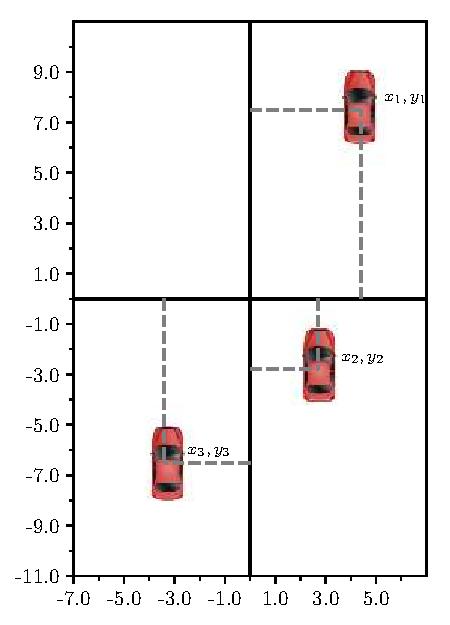
\includegraphics[width=0.25\textwidth]{img/coordinates}
	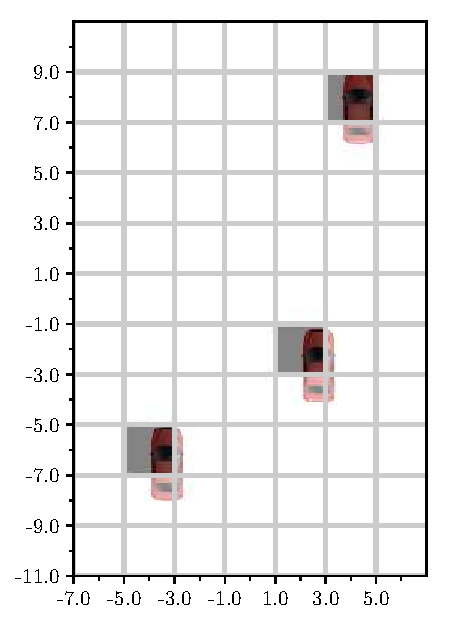
\includegraphics[width=0.25\textwidth]{img/map}
	\caption{The \emph{list of features} (left) and \emph{spatial grid} (right) representations}
	\label{fig:representation}
\end{figure}

This representation, that we call \emph{list of features}, is illustrated in \Cref{fig:representation} (left) and was used for instance in \citep{Bai2015, Gindele2015, Song2016, Sunberg2017, Paxton2017, Galceran2017, Chen2017}.


This encoding is efficient in the sense that it uses the smallest quantity of information necessary to represent the scene. However, it lacks two important properties. First, its size varies with the number of vehicles which can be problematic for the sake of function approximation which often expects constant-sized inputs. Second, we expect a driving policy $\policy$ to be \emph{permutation invariant}, i.e. not to be dependent on the order in which other traffic participants are listed. Ideally, this property should be enforced and not approximated by relying on the coverage of the $N_v!$ possible permutations $\tau$ of any given traffic state in the dataset. Formally, we require that
\begin{equation}
\label{eq:permutation}
\policy(\cdot|(s_0, s_1,\dotsc,s_{N_v})) = \policy(\cdot|(s_0, s_{\tau(1)},\dotsc,s_{\tau(N_v)})), \quad\quad\quad \forall\tau \in \mathfrak{S}_{N_v},
\end{equation}
where $\mathfrak{S}_{N_v}$ is the \emph{symmetric} group of permutations of the integer range $[1,N_v]$.
A popular way to address this limitations is to use a \emph{spatial grid} representation. Instead of explicitly representing spatial information as variables $x, y$ along with other features $f$ directly inside a state $\{s_i=(p^x_i,p^y_i,f_i)\}_{i\in[0,N]}$ indexed on the vehicles, they are instead represented implicitly through the layout of several feature variables $f_{ij}$ organised in a tensor structure, where the $(i,j)$ indexes refer to a quantisation of the 2D-space. This representation is illustrated in \Cref{fig:representation} (right). Note that the size of this tensor is related to the area covered divided by the quantisation step, which reflects a trade-off between accuracy and dimensionality.
In an occupancy grid, the $f$ features contains presence information (0-1) and additional channels such as velocity and heading, as in \citep[e.g.][]{Isele2018, Fridman2018, Bansal2018, Rehder2017c}. Another example is the use of top-view RGB images \citep[e.g.][]{Bagnell2010, Rehder2017, Rehder2017c, Liu2018}.


This permutation invariance property \eqref{eq:permutation} can also be implemented within the architecture of the policy $\pi$. A general technique to achieve this is to treat each entity similarly in the early stages -- e.g. through weight sharing -- before reducing them with a projection operator that is itself invariant to permutations, for instance a max-pooling as in \citep{Chen2017,Hoel2018} or an average as in \citep{Qi2016}. A particular instance of this idea is attention mechanisms.


\subsection{Attention mechanisms} 

The attention architecture was introduced to enable \glspl*{NN}  to discover interdepen\-dencies within a variable number of inputs.
It has been used for pedestrian trajectory forecasting in~\citep{Vemula2018} with spatiotemporal graphs and in~\citep{Sadeghian2019CVPR} with spatial and social attention using a generative \glsxtrlong{NN}. In~\citep{Sadeghian2018ECCV}, attention over top-view road scene images for car trajectory forecasting is used. Multi-head attention mechanism has been developed in~\citep{Vaswani2017} for sentence translation. In~\citep{Messaoud2019} a mechanism called non-local multi-head attention is developed. However, this is a spatial attention that does not allow vehicle-to-vehicle attention. In the present chapter, we use a multi-head social attention mechanism to capture vehicle-to-ego dependencies and build varying input size and permutation invariance into the policy model.

\section{A social attention architecture}
\label{sec:architecture}

Out of a complex scene description, the model should be able to filter information and consider only what is relevant for decision. In other words, the agent should \emph{pay attention} to vehicles that are close or conflict with the planned route.

The proposed architecture is presented in \Cref{fig:ego-architecture}. It is used to represent the $\Q$-function that will be optimized by the \gls{DQN} algorithm. It is composed of a first linear encoding layer whose weights are shared between all vehicles. At that point, the embeddings only contain individual features of size $d_x$. They are then fed to an ego-attention layer, composed of several heads stacked together. The \emph{ego} prefix highlights that it similar to a multi-head self-attention layer \citep{Vaswani2017} but with only a single output corresponding to the ego-vehicle. Such an ego-attention head is illustrated in \Cref{fig:ego-attention} and works in the following way: in order to select a subset of vehicles depending on the context, the ego-vehicle  first emits a single query $Q = [q_0]\in\Real^{1 \times d_k}$, computed with a linear projection $L_q\in\Real^{d_x \times d_k}$ of its embedding. This query is then compared to a set of keys $K = [k_0, \dots, k_{N_v}]\in\Real^{(N_v+1) \times d_k}$ containing descriptive features $k_i$ for each vehicle, again computed with a shared linear projection $L_k\in\Real^{d_x \times d_k}$. The similarity between the query $q_0$ and any key $k_i$ is assessed by their dot product $q_0 k_i^T$. These similarities are then scaled by the inverse-square-root-dimension $1/\sqrt{d_k}$\footnote{This scaling is due to the fact that the dot-product of two independent random vectors with mean 0,  variance 1, and dimension $d_k$, is a random variable with mean 0 and variance $d_k$} and normalised with a softmax function $\sigma$ across vehicles. We obtain a stochastic matrix called the \emph{attention matrix}, which is finally used to gather a set of output value $V = [v_0, \dots, v_{N_v}]$, where each value $v_i$ is a feature computed with a shared linear projection $L_v\in\Real^{d_x \times d_v}$. Overall, the attention computation for each head can be written as
\begin{equation}
\text{output}=\underbrace{\sigma\left(\frac{QK^T}{\sqrt{d_k}}\right)}_{\text{attention matrix}}V.
\label{eq:selfattention}
\end{equation}
The outputs from all heads are finally combined with a linear layer, and the resulting tensor is then added to the ego encoding as in residual networks. We can easily see that this process is permutation invariant: indeed, a permutation $\tau$ will change the order of the rows in keys $K$ and values $V$ in \eqref{eq:selfattention} but will keep their correspondence. The final result is a dot product of values and key-similarities, which is independent of the ordering.


\begin{figure}[tp]
	\centering
	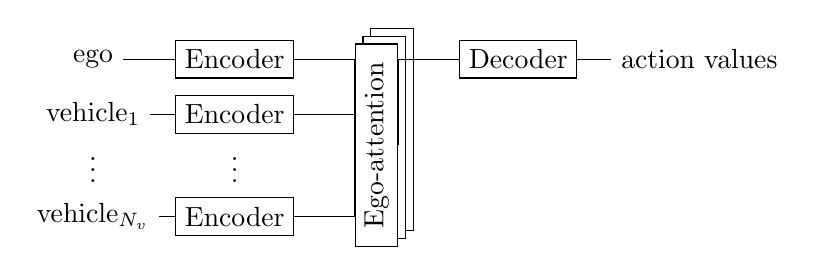
\begin{tikzpicture}
	\node(X1){ego};
	\node[below of=X1, node distance=0.7cm](X2){vehicle$_{1}$};
	\node[below of=X2, node distance=0.6cm](X3){$\vdots$};
	\node[below of=X3, node distance=0.7cm](X4){vehicle$_{N_v}$};
	
	\node[draw, right of=X1, node distance=1.8cm, rectangle](ENC1){Encoder};
	\node[draw, right of=X2, node distance=1.8cm, rectangle](ENC2){Encoder};
	\node[below of=ENC2, node distance=0.6cm](ENC3){$\vdots$};
	\node[draw, right of=X4, node distance=1.8cm, rectangle](ENC4){Encoder};
	
	\path (X1) edge (ENC1);
	\path (X2) edge (ENC2);
	\path (X4) edge (ENC4);
	
	
	\node[draw, rectangle, right of=ENC1, node distance=2.0cm, below=-0.4cm, fill=white](TRANS3){\rotatebox{90}{ Ego-attention }};
	\node[draw, rectangle, right of=ENC1, node distance=1.9cm, below=-0.3cm, fill=white](TRANS2){\rotatebox{90}{ Ego-attention }};
	\node[draw, rectangle, right of=ENC1, node distance=1.8cm, below=-0.2cm, fill=white](TRANS1){\rotatebox{90}{ Ego-attention }};
	
	\draw (ENC1.east) -| (TRANS1.west);
	\draw (ENC2.east) -| (TRANS1.west);
	\draw (ENC4.east) -| (TRANS1.west);
	
	
	\node[draw, right of=ENC1, node distance=3.6cm, rectangle](DEC1){Decoder};
	
	\draw (TRANS1.east) |- (DEC1.west);
	
	\node[right of=DEC1, node distance=2.3cm](Y1){action values};
	
	\draw (DEC1.east) -- (Y1.west);
	\end{tikzpicture}
	\caption{Block diagram of our model architecture. It is composed of several linear identical encoders, a stack of ego-attention heads, and a linear decoder.}
	\label{fig:ego-architecture}	
\end{figure}

\begin{figure}[tp]
	\centering
	\begin{tikzpicture}[scale=1, every node/.style={scale=1}]
	\node(X1){ego encoding};
	\node[below of=X1, node distance=2cm](X2){$\vdots$};
	\node[below of=X2, node distance=2cm](X3){vehicle$_{N_v}$ encoding};
	
	\coordinate[right of= X1, node distance=2cm](X1b){};
	
	\draw (X1) -- (X1b);
	
	\node[draw, right of=X1b, node distance=1cm](LK1){$L_{k}$};
	\node[draw, below of=LK1, node distance=1cm](LV1){$L_{v}$};
	\node[draw, above of=LK1, node distance=1cm](LQ1){$L_{q}$};
	
	\draw (X1b) -- (LQ1);
	\draw (X1b) -- (LK1);
	\draw (X1b) -- (LV1);
	
	
	\node[right of=LQ1, node distance=1cm](Q1){$\mathbf{q}_0$};
	\node[right of=LK1, node distance=1cm](K1){$\mathbf{k}_0$};
	\node[right of=LV1, node distance=1cm](V1){$\mathbf{v}_0$};
	
	\draw (LQ1) -- (Q1);
	\draw (LK1) -- (K1);
	\draw (LV1) -- (V1);
	
	\coordinate[right of= X3, node distance=2cm](X3b){};
	
	\draw (X3) -- (X3b);
	
	\node[draw, right of=X3b, node distance=1cm](LK3){$L_{k}$};
	\node[draw, below of=LK3, node distance=1cm](LV3){$L_{v}$};
	
	\draw (X3b) -- (LK3);	
	\draw (X3b) -- (LV3);
	
	\node[right of=LK3, node distance=1cm](K3){$\mathbf{k}_{n}$};
	\node[right of=LV3, node distance=1cm](V3){$\mathbf{v}_{n}$};
	
	\draw (LK3) -- (K3);
	\draw (LV3) -- (V3);
	
	\coordinate[right of=Q1, node distance=0.3cm](TOP){};
	\coordinate[right of=V3, node distance=0.3cm](BOT){};
	\draw[decorate,decoration={brace}] (TOP) -- node[left=5pt]{} (BOT);
	
	\node[right of=X2, text width=3cm, node distance=5.5cm](EQ){
		\footnotesize \[Q = \left( \begin{matrix}
		\mathbf{q}_0
		\end{matrix} \right)\]
		\\
		\footnotesize \[K = \left( \begin{matrix}
		\mathbf{k}_0 \\
		\vdots \\
		\mathbf{k}_{n}
		\end{matrix} \right)\]
		\\
		\footnotesize \[ V = \left( \begin{matrix}
		\mathbf{v}_0 \\
		\vdots \\
		\mathbf{v}_{n}
		\end{matrix}\right) \]
	};
	
	\node[draw, right of=X2, node distance=8.3cm](EQ2){
		\footnotesize $\sigma\left(\frac{QK^T}{\sqrt{d_k}}\right)V$};
	
	\coordinate[left of=EQ2, node distance=1.6cm, above=2.2cm](TOP2){};
	\coordinate[left of=EQ2, node distance=1.5cm, below=0.0cm](MID2){};
	\coordinate[left of=EQ2, node distance=1.6cm, below=2.2cm](BOT2){};
	\draw[decorate,decoration={brace}] (TOP2) -- node[left=5pt]{} (BOT2);
	\draw (MID2) -- (EQ2);
	
	\node[right of=EQ2, node distance=2cm](OUT){output};
	\draw (EQ2) -- (OUT);
	
	\draw[draw=black, dashed] (1.75cm, -5.5cm) rectangle (9.5cm,1.5cm);
	\end{tikzpicture}
	\caption{Architecture of an ego-attention head.
		The blocks $L_{q}$, $L_{k}$, $L_{v}$ are linear layers. The keys $K$ and values $V$ are concatenated from all vehicles, while the query $Q$ is only produced by the ego-vehicle.}
	\label{fig:ego-attention}
\end{figure}


\section{Experiments}
\paragraph{Environment}

In this experiment, we use the \href{https://github.com/eleurent/highway-env}{highway-env} environment \citep{highway-env} presented in \Cref{chapter:a}. We consider a task where vehicle-to-vehicle interaction plays a significant part: crossing a four-way intersection.
The scene -- composed of two roads crossing perpendicularly -- is populated with several traffic participants initialised with random positions, velocities, and destinations. As described in \Cref{chapter:3}, these vehicle are simulated with the Kinematic Bicycle Model, their lateral control is achieved by a low-level steering controller tracking a target route, and their longitudinal behaviour follows the \gls+{IDM} model \citep{Treiber2000}. However, this model only considers same-lane interactions and special care was required to prevent lateral collisions at the intersection. To that end, I implemented the following simplistic behaviour: each vehicle predicts the future positions of its neighbours over a three-seconds horizon by using a constant velocity model. In case of predicted collision with a neighbour, the yielding vehicle is determined based on road priorities and brakes until the collision prediction ceases. 

In this context, the agent must drive a vehicle by controlling its speed chosen from a finite set of actions $\gls+{cA} \eqdef \{\text{drive faster},\, \text{drive slower},\, \text{maintain speed}\}$. Note that the lane change actions have been removed from the general definition \eqref{eq:action-space} of \Cref{chapter:3} since the roads are all single-lane in this example. The lateral control is performed automatically by a low-level controller, such that the problem complexity is focused on the high-level interactions with other vehicles, namely the decision to either give or take way. The reward function $\gls+{reward}$ is defined as in \eqref{eq:reward-function}.

\paragraph{Agents}

We evaluate three different agents, whose characteristics are summarised in \Cref{tab:agents}.
\begin{itemize}
	\item \MLPL: a \emph{list of features} state representation is used, as described in \Cref{sec:background}. The model is a simple \gls{FCN}. Because this architecture requires a fixed-size input, we use zero-padding to fill the input tensor up to a maximum number $N=14$ of observed vehicles, and add an additional \emph{presence} feature to the coordinates described in \eqref{eq:coordinates} so as to identify active rows.
	\item \CNNG: a \emph{spatial grid} representation is used, as described in \Cref{sec:background}, with a $32 \times 32$ grid where each cell represents a $2\text{m}\times 2$m square. The model is a \gls{CNN}.
	\item \EgoAtt: a \emph{list of features} state representation is used along with the Ego-Attention architecture described in \Cref{sec:architecture}. As this model supports varying-size inputs, zero-padding is not required.
\end{itemize}

\begin{table}[tp]
	\centering
	\begin{threeparttable}
		\caption{Characteristics of the agents}
		\label{tab:agents}
		\begin{tabular}{lccc}
			\toprule
			Architecture & \MLPL & \CNNG & \EgoAtt \\
			\midrule 
			Input sizes & [15, 7] & [32, 32, 7] & [~$\boldsymbol{\cdot}$~, 7] \\
			Layers sizes & [128, 128] &  \makecell[tc]{Convolutional layers: 3 \\ Kernel Size: 2 \\
				Stride: 2 \\ Head: [20]} & \makecell[tl]{Encoder: [64, 64] \\Attention: 2 heads\\\phantom{Attention: }$d_k=32$ \\ Decoder: [64, 64]} \\
			Number of parameters & 3.0e4 & 3.2e4 & 3.4e4 \\
			Variable input size & No & No &  {Yes}  \\
			Permutation invariant & No & {Yes} &  {Yes} \\
			\bottomrule
		\end{tabular}
	\end{threeparttable}
\end{table}

These agents are all trained with the \gls{DQN} algorithm using the same hyperparameters, and their architectures are scaled to admit about the same number of trainable parameters for fair comparison.

\paragraph{Performances}

We plot in \Cref{fig:attention-results} the evolution of the total reward, episode length and average velocity during training, over 4000 episodes and repeated across 120 random seeds.
The \MLPL agent learns to accelerate to earn short-term rewards, as shown by its high average velocity, but fails to exploit the information of other vehicles and crashes often, leading to short episodes. We obtain a risky and blind policy that is the worst performing.
Conversely, the \CNNG architecture benefits from its invariance to permutations and manages to learn to brake upon arrival at the intersection to avoid collisions, as we can see from its higher episode length. However, it only proceeds when the intersection has been fully cleared, as reflected by its low average velocity. This results in an overly cautious policy -- a common trait colloquially known as the \emph{freezing robot problem} \citep{Trautman2010} -- with a slight increase in performance.
In stark contrast, the \EgoAtt policy quickly learns both when it must slow down at the intersection (see the high episode length), but also when it can exploit the gaps in the traffic and take way to vehicles that are far or slow enough (see the higher average velocity than \CNNG). This translates as a significant performance improvement, and the overall resulting behaviour is qualitatively more nuanced and human-like.

\begin{figure}[htp]
	\centering
	\begin{subfigure}[t]{0.6\linewidth}
		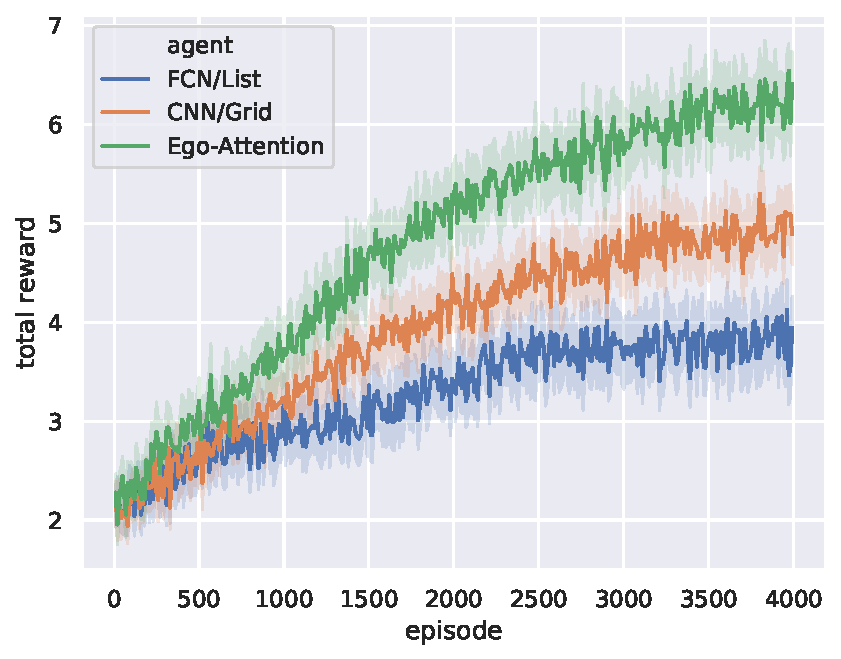
\includegraphics[width=\linewidth]{img/total_reward}
		\caption{Average return $\return=\sum_t\gamma^t\R(s_t,a_t)$ (higher is better)}
		\label{fig:attention-reward}
	\end{subfigure}
	\begin{subfigure}[t]{0.49\linewidth}
		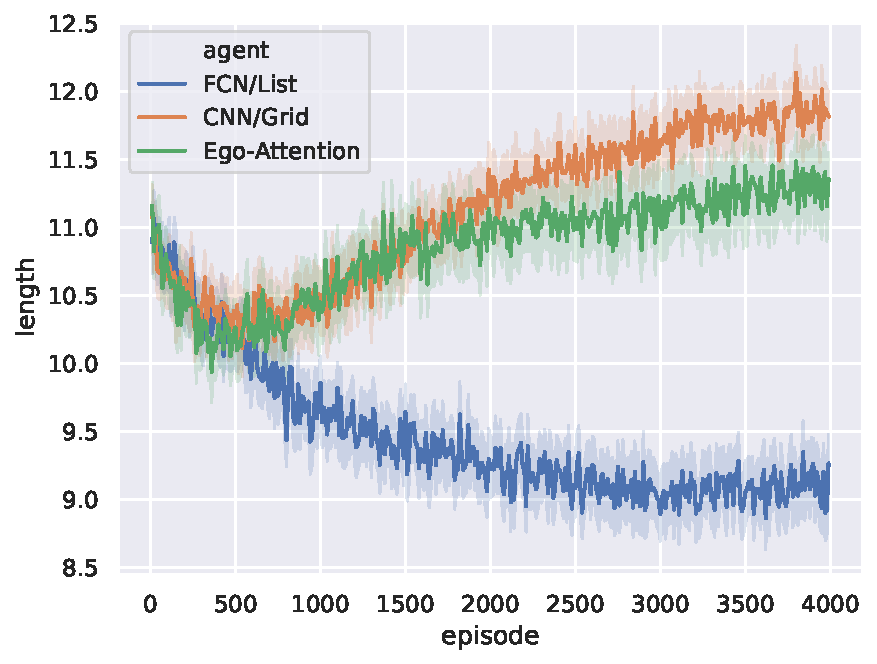
\includegraphics[width=\linewidth]{img/length}
		\caption{Average episode length. Higher is better, since episodes are terminated at collisions (or after 13 steps).}
		\label{fig:attention-length}
	\end{subfigure}
	\begin{subfigure}[t]{0.49\linewidth}
		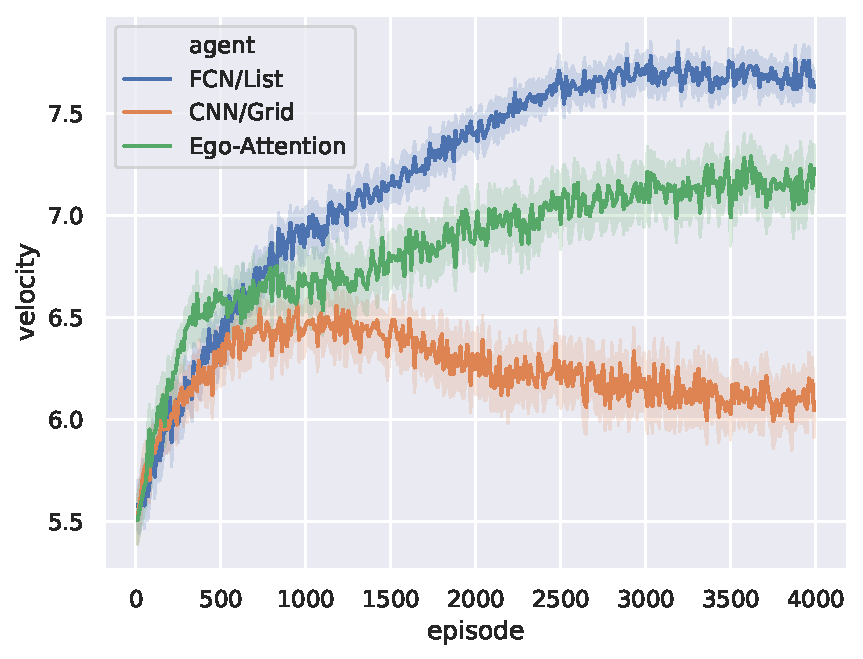
\includegraphics[width=\linewidth]{img/velocity}
		\caption{Average speed $v_0$ of the ego-vehicle (higher is better)}
		\label{fig:attention-velocity}
	\end{subfigure}
	\caption{Performances of the tree agents according to various measures. We display the mean values -- along with their 95\% confidence interval -- averaged over 120 random seeds.}
	\label{fig:attention-results}
\end{figure}

\paragraph{Attention interpretation}

In any given state, the attention matrix can be visualised in the following way: we connect the ego-vehicle to every vehicle by a line of width proportional to the corresponding attention weight. Since the architecture can contain several ego-attention heads, we use different colours to distinguish them. In our experiments, two attention heads were used and will be represented in green and blue. We observe in \Cref{fig:heads} that they specialised to focus on different areas: the green head is only watching the vehicles coming from the left, while the blue head restricts itself to vehicles in the front and right directions. However, we notice that both heads exhibit a common behaviour: they direct their attention to incoming vehicles that are likely to collide with the ego-vehicle, depending on their current position, heading, velocity, and ignore those that are too far or in a conflict-less situation. In particular, the attention tends to increase when vehicles get closer, as shown in \Cref{fig:distance}; also available in video \footnote{\href{https://eleurent.github.io/social-attention/assets/2\_distance.mp4}{https://eleurent.github.io/social-attention/assets/2\_distance.mp4}}. It can also be very sensitive to small variations in the traffic state, as reflected in \Cref{fig:sensitivity}. A full episode showcasing interactions with several vehicles is shown in \Cref{fig:episode}; a video is also available\footnote{\href{https://eleurent.github.io/social-attention/assets/1\_episode.mp4}{https://eleurent.github.io/social-attention/assets/1\_episode.mp4}}.


\begin{figure}[tp]
	\centering
	\begin{minipage}{.44\textwidth}
		\centering
		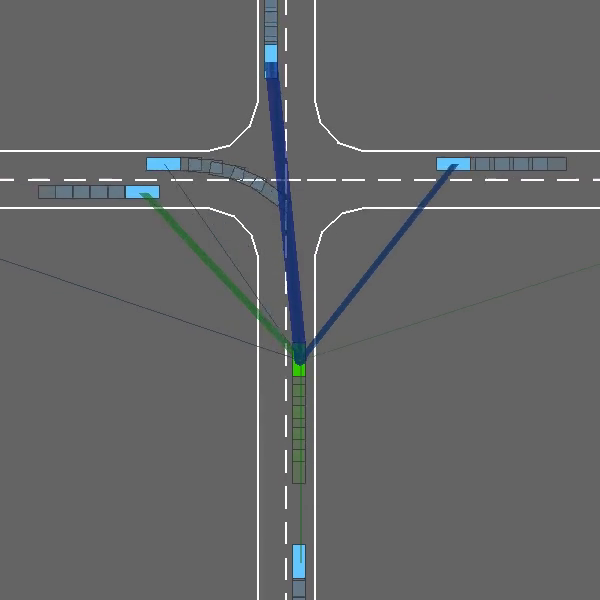
\includegraphics[width=\linewidth]{img/head_specialization}
		\captionof{figure}{The attention heads specialised in different areas: left and front/right.}
		\label{fig:heads}
	\end{minipage}
	\hfill
	\begin{minipage}{.545\textwidth}
		\centering
		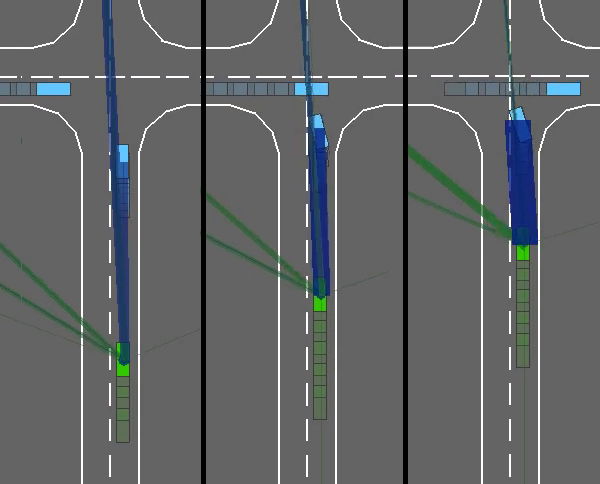
\includegraphics[width=\linewidth]{img/distances}
		\captionof{figure}{The attention paid to a vehicle tends to increase as it gets closer.}
		\label{fig:distance}
	\end{minipage}
\end{figure}

\begin{figure}[tp]
	\centering
	\begin{subfigure}[t]{0.4\linewidth}
		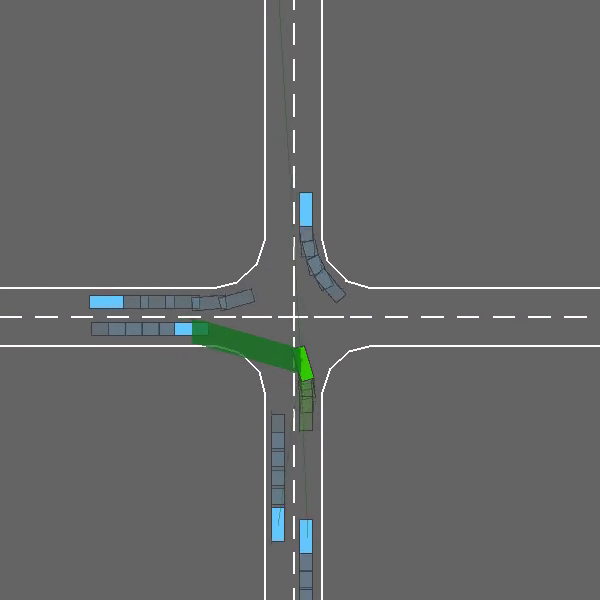
\includegraphics[width=\linewidth]{img/watch1}
		\caption{The agent has stopped at the intersection, its attention is focused on an incoming vehicle whose destination is still uncertain.}
	\end{subfigure}
	\begin{subfigure}[t]{0.4\linewidth}
		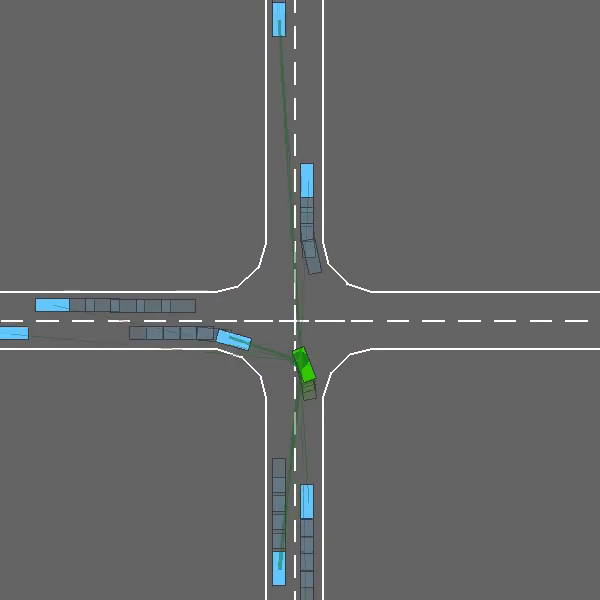
\includegraphics[width=\linewidth]{img/watch2}
		\caption{As soon as the vehicle orientation changes, revealing its intention of turning right, the attention drops and the agent starts accelerating right away.}
	\end{subfigure}
	\caption{Sensitivity to uncertainty.}
	\label{fig:sensitivity}
\end{figure}

\begin{figure}[tp]
	\centering
	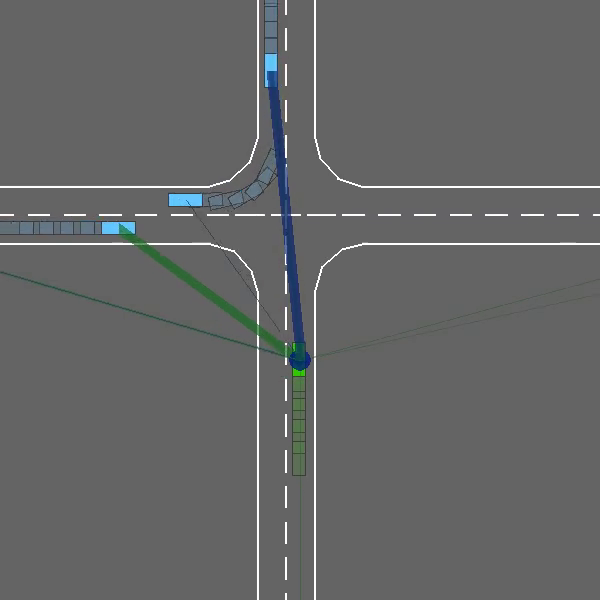
\includegraphics[width=.32\linewidth]{img/episode1}
	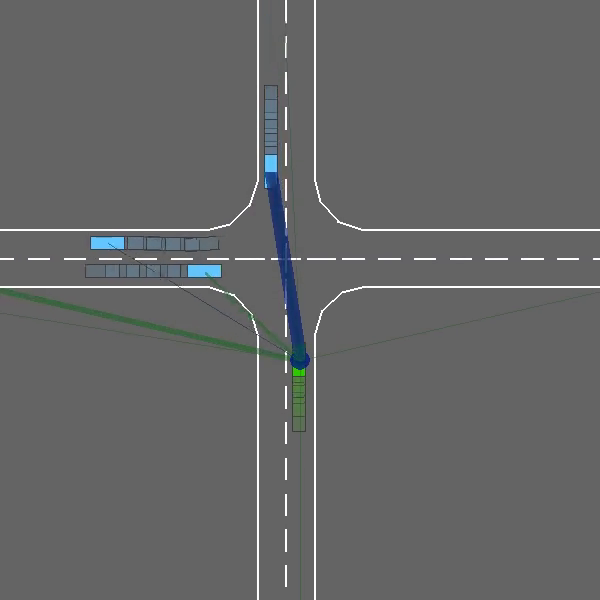
\includegraphics[width=.32\linewidth]{img/episode2}
	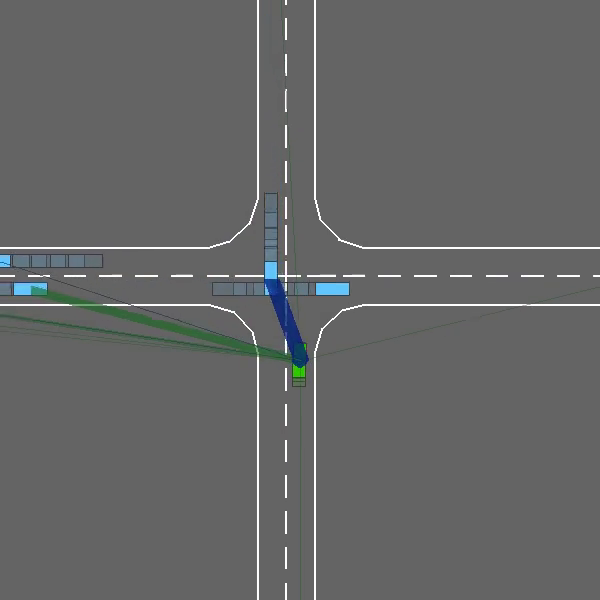
\includegraphics[width=.32\linewidth]{img/episode3}
	\\[0.12em]
	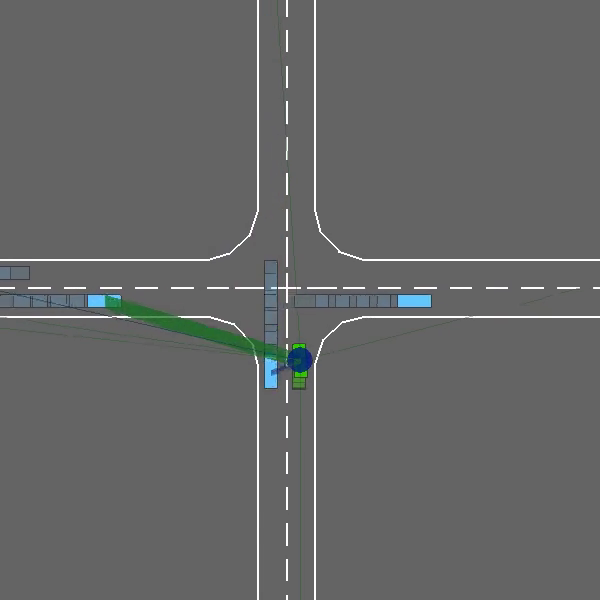
\includegraphics[width=.32\linewidth]{img/episode4}
	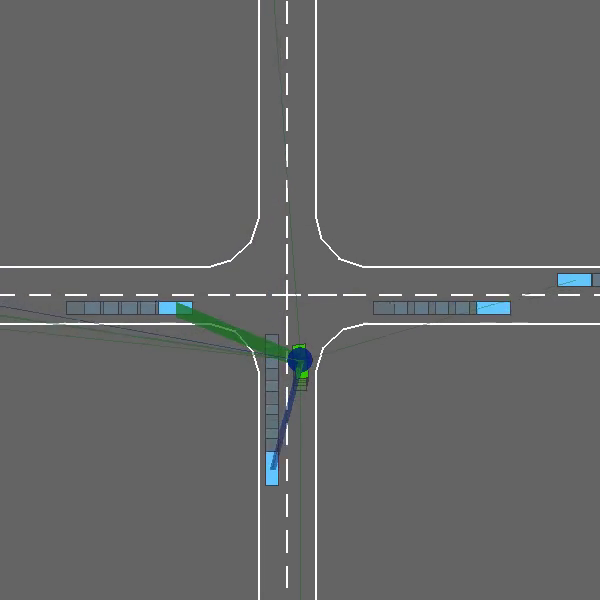
\includegraphics[width=.32\linewidth]{img/episode5}
	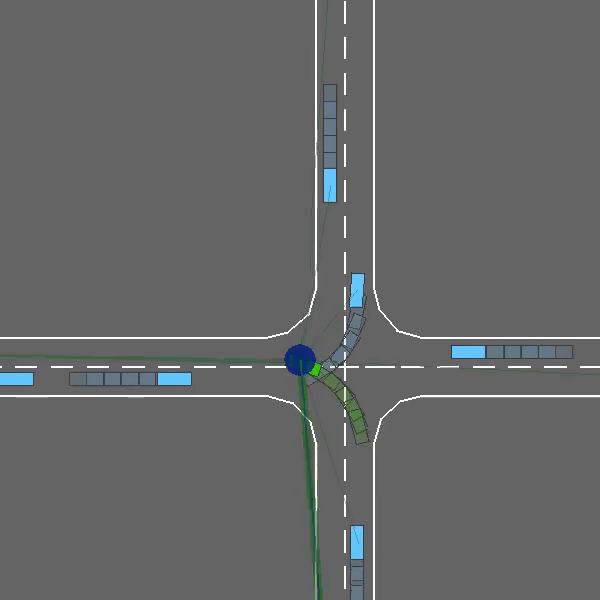
\includegraphics[width=.32\linewidth]{img/episode6}
	\caption[A complete episode.]{A complete episode. \emph{From left to right, top to bottom}: 
		\begin{enumerate*}
			\item The green and blue heads direct their attentions to the left and front vehicles, respectively;
			\item The left-vehicle is passing and is no longer a threat;
			\item Immediately, the green attention head switches to the next vehicle coming from the left;
			\item The front vehicle has now passed, and the blue attention head is now focused on the ego-vehicle;
			\item The ego-vehicle waits for one last vehicle coming from the left
			\item The ego-vehicle can finally proceed, and its attention is focused on itself.
		\end{enumerate*}
}
	\label{fig:episode}
\end{figure}

\paragraph{Exploiting interaction patterns}

The agent decisions regarding right of way are not enforced through rewards but interactions: based on the defined road priorities, some vehicles will take way to the ego-vehicle while others will not. By changing which is a priority road, we can influence the rules of interactions which affects the learnt behaviour. In \Cref{fig:priority}, we compare two policies placed in the exact same initial state and observe how their decisions are affected by their internal model of how incoming vehicles interact with them. This difference showcases the ability of our proposed architecture to discover and exploit such interaction patterns.

\begin{figure}[htp]
	\centering
	\begin{subfigure}[t]{0.48\linewidth}
		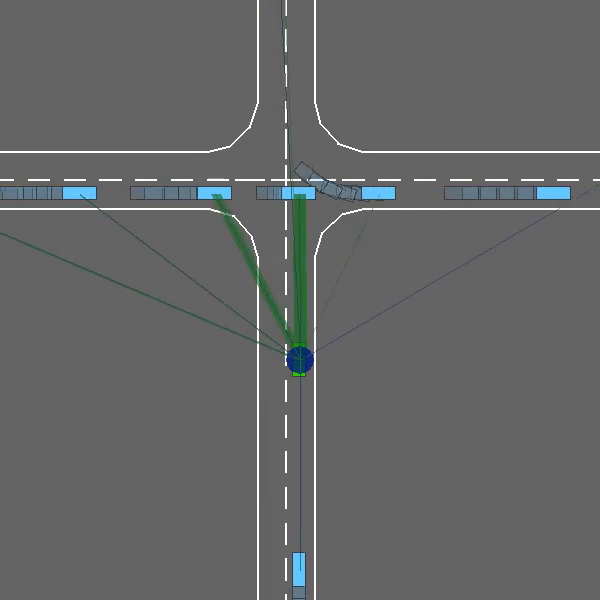
\includegraphics[width=\linewidth]{img/priority1}
		\caption{When trained on a non-priority road, the agent learns to yield to incoming vehicles.}
	\end{subfigure}
	\begin{subfigure}[t]{0.48\linewidth}
		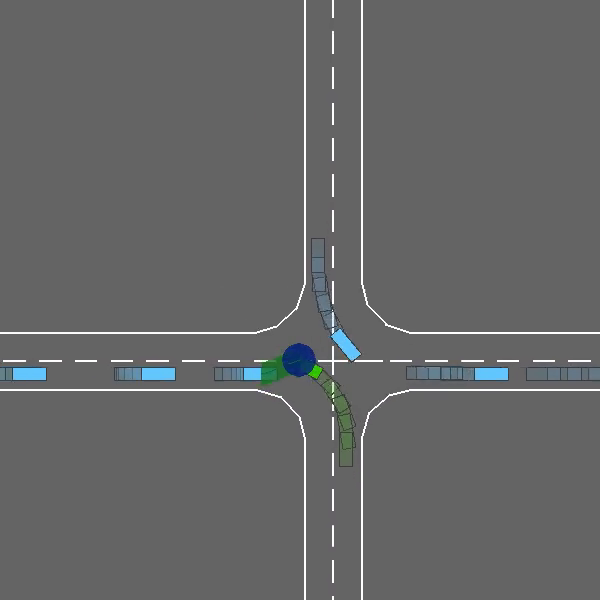
\includegraphics[width=\linewidth]{img/priority2}
		\caption{When trained on a priority road, the agent expects other vehicles to give way and is consequently more aggressive.}
	\end{subfigure}
	\caption{Effect of the right of way.}
	\label{fig:priority}
\end{figure}

\paragraph{Goal conditioning}

In the previous examples, we trained a policy tailored for left-turns only because it is the hardest direction with the most conflict points and the lowest priority level. Two individual policies tailored for right turns and driving straight can be trained as well, with similar results. Training a generic intersection policy would be less efficient without any prior information on where the ego-vehicle is headed. To remedy this problem, the destination could be added as additional features in \eqref{eq:coordinates}, for instance encoded as a desired direction $(d_x, d_y)$. This destination feature could also be used for other traffic participants to encode blinker information when available. This should result in a more efficient and generic policy.

\section*{Chapter conclusion}

In this chapter, we showed that the \emph{list of features} representation, commonly used to describe vehicles in autonomous driving literature, is not tailored for use in a function approximation setting, in particular with neural networks. These concerns can be addressed by the \emph{spatial grid} representation, but at the price of an increased input size and loss of accuracy. In contrast, we proposed an attention-based neural network architecture to tackle the aforementioned issues of the \emph{list of features} representation without compromising either size or accuracy. This architecture enjoys a better performance on a simulated negotiation and intersection crossing task, and is also more interpretable thanks to the visualisation of the attention matrix. The resulting policy successfully learns to recognise and exploit the interaction patterns that govern the nearby traffic.

Let us back up a moment and reflect again on the behaviours exhibited by \Cref{fig:attention-results}. Though \EgoAtt performs better than \CNNG, it also has shorter episodes, which means it collides more often with other vehicles. Though this {aggressive} behaviour is deemed better by our choice of reward function, it may not be desirable in practice. A straightforward way to make the optimal policy more {conservative} is to manually tune the reward function and increase the weight of collisions. However, setting too high a penalty may also result in overly {cautious} behaviours. Finding the sweet spot between these two extremes can be difficult and demanding since changing the reward requires retraining the policy entirely. In the next chapter, we study a way to learn not a single policy but rather a whole range of policies that exhibit different levels of risk.


%!TEX root = ../../PhD_thesis__Edouard_Leurent.tex

\graphicspath{{2-Chapters/5-Chapter/}}

\chapter{Acting under Adjustable Constraints}
\label{chapter:5}

\begin{flushright}
	\begin{tabular}{@{}l@{}}
		\emph{If you can meet with Triumph and Disaster}\\
		\emph{And treat those two impostors just the same;}\\
		\dots\dots\dots\dots\dots\dots\dots\dots\dots\dots\dots\dots\dots\dots\dots\dots\\
		\emph{If you can make one heap of all your winnings}\\
		\emph{And risk it on one turn of pitch-and-toss}\\
	\end{tabular}

%	Rudyard Kipling, \href{https://eleurent.github.io/sisyphe/texts/if-.html}{\enquote{If--}}. \emph{Rewards and Fairies}.
	Rudyard Kipling, \href{https://eleurent.github.io/sisyphe/texts/if-.html}{\emph{If--}}.
\end{flushright}

%\begin{flushright}
%	\begin{tabular}{@{}l@{}}
%		\emph{Phlebas the Ph\oe{}nician, a fortnight dead,}\\
%		\emph{Forgot the cry of gulls, and the deep sea swell}\\
%		\emph{And the profit and loss.}\\
%	\end{tabular}
%
%	T. S. Eliot, \href{https://www.poetryfoundation.org/poems/47311/the-waste-land}{\emph{The Waste Land}}.	
%\end{flushright}

\abstractStartChapter{}%
  When we drive, we must comply with two contradictory objectives: \textit{efficiency} and \textit{safety}. In this chapter, we strive to reconcile them by formalising a first notion of \textit{risk}. We consider \glspl+{BMDP}, in which risk is implemented as a cost signal constrained to lie below an \emph{adjustable} threshold. The latter provides the system manufacturer with a slider allowing them to adjust in real-time the level of risk taken by the vehicle. So far, \glspl{BMDP} could only be solved in the case of known dynamics and finite state spaces, which is not suitable for our application which features continuous kinematic states and unknown human behaviours. This chapter extends the state-of-the-art to continuous spaces and unknown dynamics. %We show that the solution to a \gls{BMDP} is a fixed point of a novel Budgeted Bellman Optimality operator. This observation allows us to introduce a natural extension of Deep Reinforcement Learning algorithms to address large-scale \glspl{BMDP}. 
  Our approach is motivated by the prospect of training a risk-sensitive driving policy for a two-way road, where overtaking a vehicle requires driving on the wrong lane.\footnote{This chapter is based on an article published in the proceedings of the \emph{32nd conference on advances in Neural Information Processing Systems (NeurIPS)} \citep{CarraraLeurent2019}. It is joint work with Nicolas Carrara, who came up with the algorithm and carried-out the dialogue experiment. I did most of the theoretical analysis, the driving experiment; and we worked together on the exploration procedure and scaling-up the implementation.}
\minitocStartChapterNoNewPage{}

\section{Motivation}

As stated in \Cref{chapter:1}, \glsxtrlong{RL} is a general framework for decision-making under uncertainty. Formally, we seek a policy $\policy\in\cM(\cA)^{\cS}$ that maximises in expectation the $\discountfactor$-discounted return of rewards $\return^{\policy} = \sum_{t=0}^\infty \discountfactor^t \reward(s_t, a_t)$.

However, this modelling assumption comes at a price: no control is given over the spread of the performance distribution \citep{Dann2018}. In many critical real-world applications, including \glsxtrlong{AD}, failures may turn out very costly. This is an issue as most decision-makers would rather give away some amount of expected optimality to increase the performances in the lower-tail of the distribution. As discussed in \Cref{chapter:2}, this has led to the development of several risk-averse variants where the optimisation criteria include other statistics of the performance, such as the worst-case realisation \citep{Iyengar2005,Nilim2005,Wiesemann2013}, the variance-penalised expectation \citep{Tamar2012,Garcia2015}, the Value at Risk \citep{Mausser2003,Luenberger2013}, or the Conditional Value at Risk \citep{Chow2014,Chow2018}.

\glsxtrlong{RL} also assumes that the performance can be described by a single reward function $\reward$. Conversely, real problems typically involve many aspects, some of which can be contradictory \citep{Liu2014}. In our case, a self-driving car needs to balance between progressing quickly on the road and avoiding collisions. In \gls{MORL}, each of these aspects is independently modelled by a separate reward signal. Then, the set of policies is partitioned into 
\begin{enumerate*}[label=(\roman*)]
	\item the class of \emph{dominated} policies $\policy$, for which there exists an \emph{improvement}, \ie another policy $\policy'$ with at least some objectives increased, and none decreased;
	\item the \emph{Pareto front} $\Pi^\star$, of undominated policies, illustrated in \Cref{fig:pareto-front}.
\end{enumerate*}

\begin{figure}[ht]
\centering
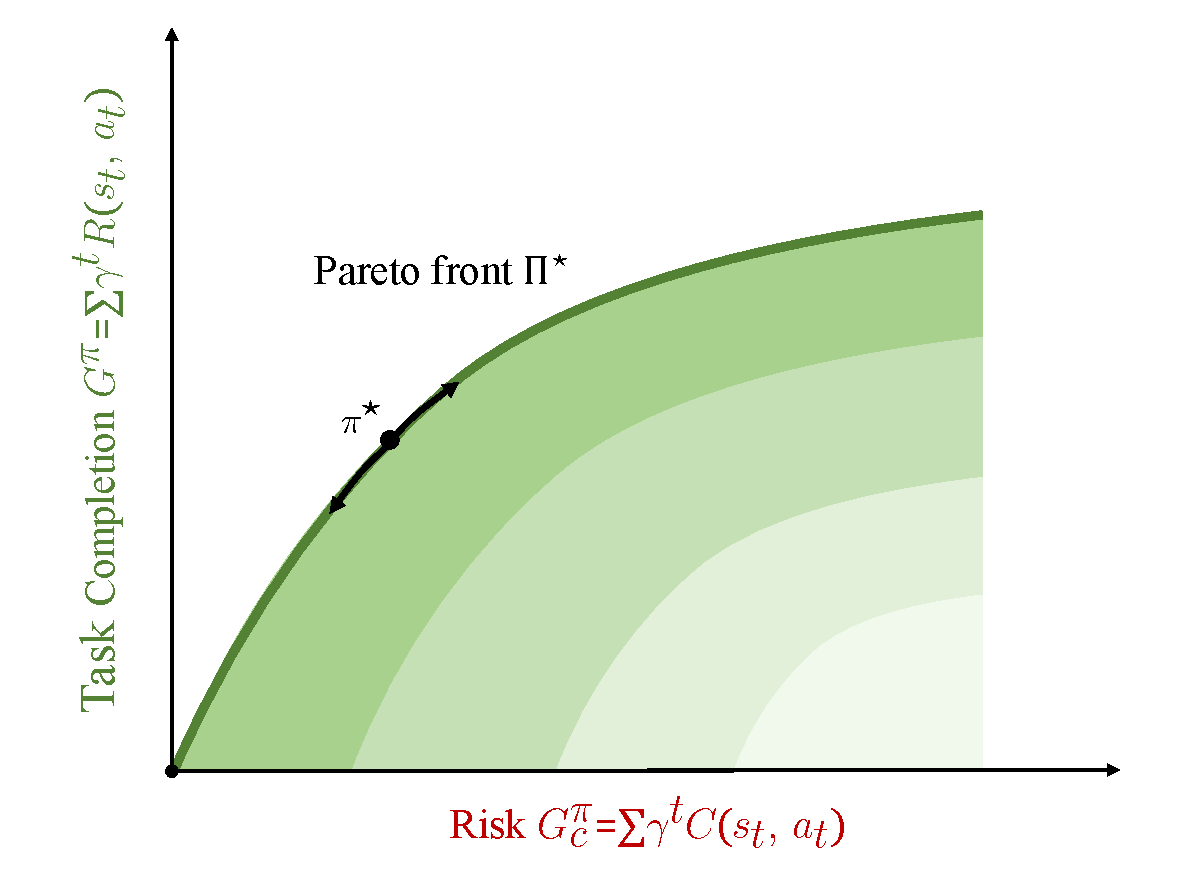
\includegraphics[width=0.55\linewidth]{img/pareto1}
\caption{A \gls{MOMDP} with two objectives: the rewards $R$ must be maximised, while the costs $C$ must be minimised. The policies are partitioned into dominated policies, shown in light shades of green, and the Pareto front $\Pi^\star$, shown in dark green. Cautious policies with low efficiency and risk are located on the bottom-left, while aggressive policies with high efficiency and risk are on the top-right.}
\label{fig:pareto-front}
\end{figure}

A standard way to cast a \gls+{MOMDP} into an \gls{MDP} is to aggregate several objectives in a single reward function \citep{Roijers2013ASO}. However, this does not allow to explicitly control the trade-off between the different objectives, since higher rewards can compensate for higher penalties. For instance, if a weighted sum is used to balance velocity $v$ and crashes $c$, then for any given choice of weights $\omega$ the optimality equation $\omega_v\expectedvalue[\sum\discountfactor^t v_t] + \omega_a\expectedvalue[\sum\discountfactor^t c_t] = \return^{\star} = \max_{\policy} \return^{\policy}$ is the equation of a line in $(\expectedvalue[\sum\discountfactor^t v_t], \expectedvalue[\sum\discountfactor^t c_t])$, and the automotive company cannot control where its optimal policy $\optimalpolicy$ lies on that line. 

Both of these concerns are addressed in the \glsfirst+{CMDP} setting \citep{Beutler1985,Altman1999}, illustrated in \Cref{fig:cmdp}. In this multi-objective formulation, \hlg{task completion} and \hlr{safety} are considered separately. We equip the \gls{MDP} with a cost signal $\hlr{\constraint} \in \Real^{\cS\times \cA}$ and a cost {budget} $\hlb{\budget}\in\Real$. Similarly to $\hlg{\return^{\policy}}$, we define the return of costs $\hlrb{\constraintreturn[^{\policy}]} = \sum_{t=0}^\infty \discountfactor^t \constraint(s_t, a_t)$ and the new cost-constrained objective:
\begin{equation}
\label{eq:cmdp}
\begin{array}{lcr}
\displaystyle \max_{\policy\in\cM(\cA)^{\cS}} \expectedvalue[\hlgb{\return^{\policy}} | s_0=s] & \text{ s.t. } & \expectedvalue[\hlrb{\constraintreturn[^{\policy}]} | s_0=s] \leq \hlbb{\budget}
\end{array}
\end{equation}
This constrained framework allows for better control of the performance-safety trade-off. However, it suffers from a major limitation: the \idx{budget} has to be chosen before training, and cannot be changed afterwards.


\begin{figure}[ht]
\begin{subfigure}[t]{0.48\linewidth}
	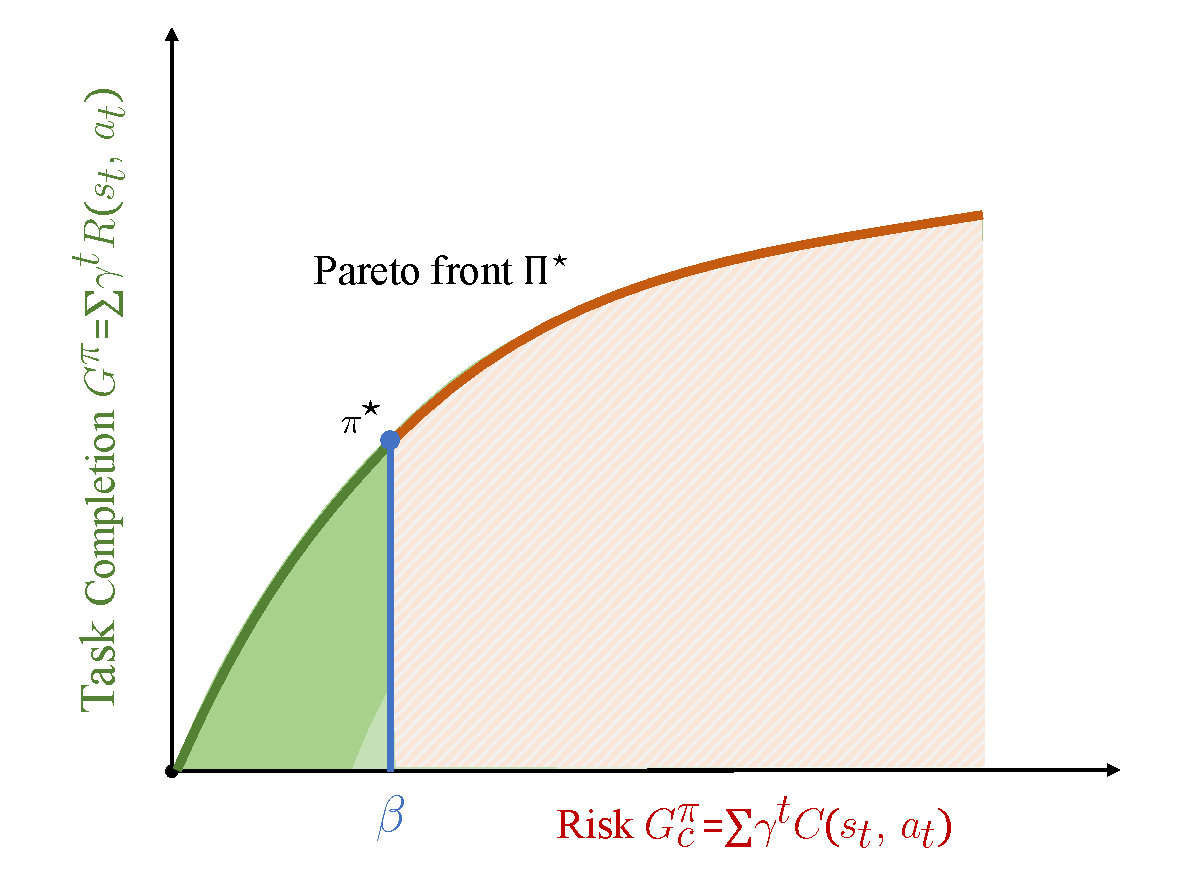
\includegraphics[width=\linewidth]{img/pareto2}
	\caption{In a \glsxtrshort{CMDP}, we learn a single policy $\pi^\star$ (\hlb{blue dot $\bullet$}) with a fixed expected risk $\budget\in\budgetspace$}
	\label{fig:cmdp}
\end{subfigure}\hfill
\begin{subfigure}[t]{0.48\linewidth}
	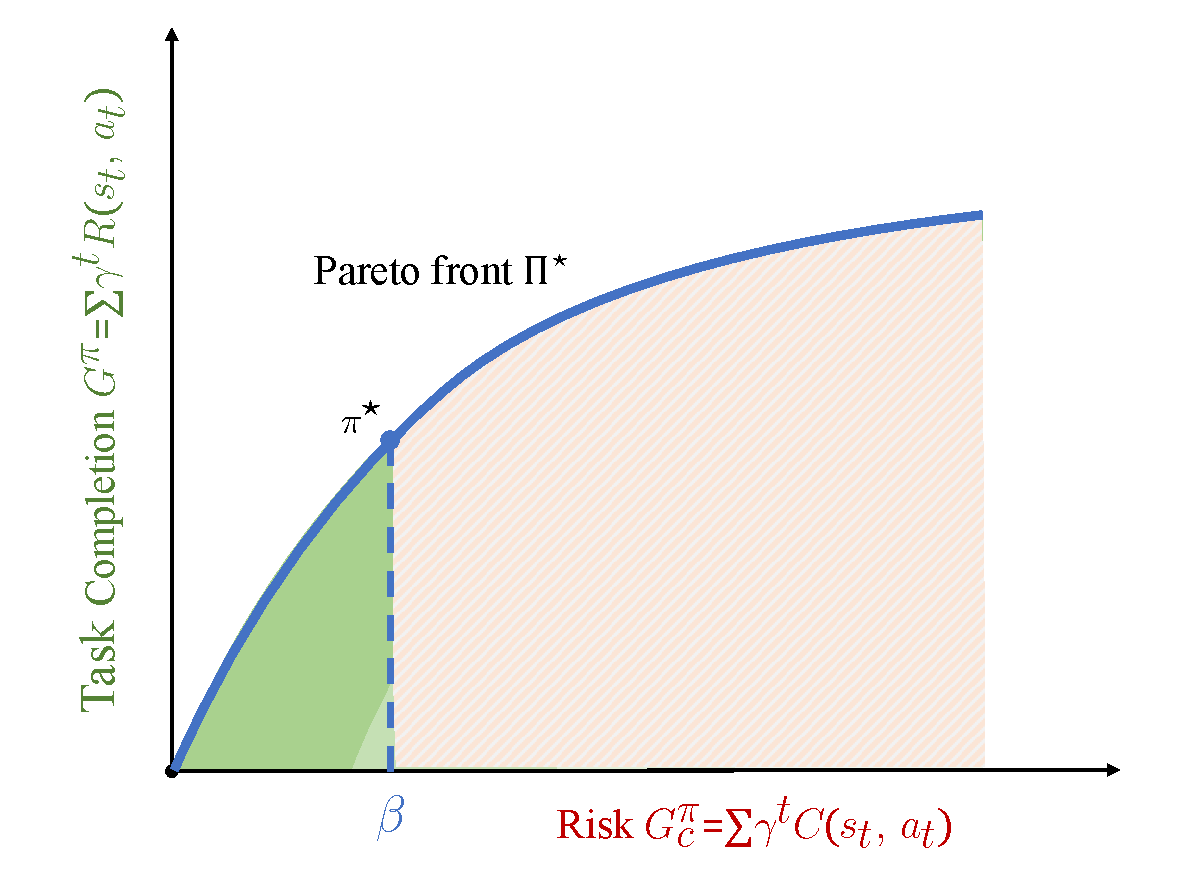
\includegraphics[width=\linewidth]{img/pareto3}
	\caption{In a \glsxtrshort{BMDP}, we learn a set $\Pi^\star$ of policies called the Pareto front (\hlb{blue frontier --}), for the whole range $\budgetspace$ of allowed risks}
	\label{fig:bmdp}
\end{subfigure}
\caption{Comparison between the \gls{CMDP} and \gls{BMDP} frameworks.}
\end{figure}

To tackle this issue, the \glsfirst+{BMDP} was introduced in \citep{Boutilier_Lu:uai16} as an extension of \glspl{CMDP} to enable the online control over the {budget} $\budget$ within a closed interval $\budgetspace \subset \Real$ of admissible budgets\index{budget}. Instead of fixing the {budget} prior to training, the objective is now to find a generic optimal policy $\optimalpolicy$ that takes $\budget$ as input so as to solve the corresponding \gls{CMDP} \eqref{eq:cmdp} for all budgets $\budget\in\budgetspace$. This gives the system designer the ability to move in real-time the optimal policy $\optimalpolicy$ along the Pareto front of the different reward-cost trade-offs, as shown in \Cref{fig:bmdp}.

In the seminal work of \citet{Boutilier_Lu:uai16}, \glspl{BMDP} were originally studied in the context of finite states $\cS$, finite horizon, and known \gls{BMDP} parameters. Our first contribution is to re-frame the \gls{BMDP} formulation in the context of continuous states and infinite discounted horizon. We then propose a novel Budgeted Bellman Optimality Operator and prove the optimal value function to be a fixed point of this operator. Second, we use this operator in \gls{BFTQ}, a {batch} \gls{RL} algorithm, for solving \glspl{BMDP} {online}, without prior knowledge of the $(\Ps, \reward, \constraint)$ parameters, by interacting with an {environment}. Third, we scale this algorithm to large problems by (i) providing an efficient implementation of the Budgeted Bellman Optimality operator based on convex programming, (ii) a tailored risk-sensitive exploration procedure, and (iii) leveraging tools from Deep \glsxtrlong{RL} such as \glsxtrlongpl{NN} for function approximation and synchronous parallel computing. Finally, we validate our approach in two {environment}s that display a clear trade-off between rewards and costs: a dialogue system example, and a behavioural planning problem for overtaking on a two-way road. 

\section{Budgeted dynamic programming}
\label{sec:bdp}
We work in the space of budgeted policies\index{budgeted policy}, where $\policy$ both depends on $\budget$ and also outputs the next budget $\budgetaction$. Hence, the budget $\budget$ is neither fixed nor constant as in the \gls{CMDP} setting but instead evolves as part of the dynamics.

We cast the \gls{BMDP} problem as a \gls{MOMDP} problem \citep{Roijers2013ASO} by considering \emph{augmented} state and action spaces $\ocS = \cS\times \budgetspace$ and $\ocA= \cA\times \budgetspace$, and equip them with the augmented dynamics $\augmentedtransition\in \cM(\ocS)^{\ocS \times \ocA}$ defined as:
\begin{equation}
\augmentedtransition\left(\os' \condbar \os, \oa\right) = \augmentedtransition\left((s',\budget') \condbar (s,\budget), (a, \budgetaction)\right) \eqdef \Ps(s'|s, a)\dirac(\budget' - \budgetaction),
\end{equation}
where $\dirac$ is the Dirac indicator distribution.

In other words, in these augmented dynamics, the output budget $\budgetaction$ returned at time $t$ by a \idx{budgeted policy} $\budgetedpolicy\in \policies=\cM(\ocA)^{\ocS}$ will be used to condition the policy at the next timestep $t+1$.

We stack the rewards and cost functions in a single \emph{vectorial} signal $\oR \in (\Real^2)^{{\ocS \times \ocA}}$:

\begin{definition}
	\begin{leftbar}[defnbar]
	Given an augmented transition $(\os, \oa) =((s,\budget), (a, \budgetaction))$, we define
	\begin{equation}
	\gls+{oR}(\os, \oa) \eqdef  \begin{bmatrix}
	\hlg{\R(s, a)}\\
	\hlr{\constraint(s, a)}
	\end{bmatrix}\in\Real^2.
	\end{equation}
	\end{leftbar}
\end{definition}

Likewise, we augment the return:

\begin{definition}
	\begin{leftbar}[defnbar]
	The return $\augmentedreturn[^{\budgetedpolicy}] = (\return[^{\budgetedpolicy}], \constraintreturn[^{\budgetedpolicy}])$ of a \idx{budgeted policy} $\budgetedpolicy\in\policies$ refers to
	\begin{equation}
	\gls+{augmentedreturn}[^{\budgetedpolicy}] \eqdef \sum_{t=0}^\infty \discountfactor^t \oR(\os_t, \oa_t).
	\end{equation}
	\end{leftbar}
\end{definition}

as well as the value functions:

\begin{definition}
	\begin{leftbar}[defnbar]
	The value functions $\oV[^{\budgetedpolicy}]$, $\oQ[^{\budgetedpolicy}]$ of a \idx{budgeted policy} $\budgetedpolicy\in\policies$ are defined as
	\begin{align}
	\begin{split}
	\label{eq:value-function}
	\gls+{oV}[^{\budgetedpolicy}](\os) &= (\hlg{\Vr[^\budgetedpolicy]}, \hlr{\Vc[^\budgetedpolicy]}) \eqdef \expectedvalue\left[ \augmentedreturn^{\budgetedpolicy} \condbar \ov{s_0} = \os\right] \\
	\gls+{oQ}[^{\budgetedpolicy}](\os, \oa) &= (\hlg{\Qr[^\budgetedpolicy]}, \hlr{\Qc[^\budgetedpolicy]}) \eqdef \expectedvalue\left[ \augmentedreturn^{\budgetedpolicy} \condbar \ov{s_0} = \os, \ov{a_0} = \oa\right].
	\end{split}
	\end{align}
	\end{leftbar}
\end{definition}

We restrict $\ocS$ to feasible budgets only: $\ocS_f \eqdef \{(s,\budget)\in\ocS: \exists \budgetedpolicy\in\policies, \Vc[^\budgetedpolicy](s) \leq \budget\}$ that we assume to be non-empty for the \gls{BMDP} to admit a solution. We still write $\ocS$ in place of $\ocS_f$ for brevity of notations.

\begin{proposition}[Budgeted Bellman Expectation]
	\begin{leftbar}[propositionbar]
	\label{prop:bellman-expectation}
	The value functions $\oV^{\budgetedpolicy}$ and $ \oQ^{\budgetedpolicy}$ verify:
	\begin{align}
	\oV^{\budgetedpolicy}(\os) = \sum_{\oa\in\ocA}\budgetedpolicy(\oa | \os) \oQ^{\budgetedpolicy}(\os, \oa) \qquad \oQ^{\budgetedpolicy}(\os, \oa) = \gls{oR}(\os, \oa) + \discountfactor\sum_{\os'\in\ocS}\augmentedtransition\left(\os' \condbar \os, \oa\right) \oV^{\budgetedpolicy}(\os'). \label{eq:bellman_expectation}
	\end{align}
	Moreover, consider the Budgeted Bellman Evaluation\index{Bellman Evaluation} operator $\abo^{\gls+{budgetedpolicy}}$:
	$\forall \oQ\in(\Real^2)^{\ocS\ocA}, \os\in\ocS, \oa\in\ocA$,
	\begin{align}
	\label{eq:bellman_expectation_operator}
	\gls+{abo}^{\gls+{budgetedpolicy}} \oQ(\os, \oa) &\eqdef \gls{oR}(\os, \oa) + \discountfactor \sum_{\os'\in\ocS}\sum_{\oa'\in\ocA}\augmentedtransition(\os'|\os, \oa)\budgetedpolicy(\oa'|\os') \oQ(\os', \oa').
	\end{align}
	Then $\abo^{\budgetedpolicy}$ is a $\discountfactor$-contraction and $\oQ^{\budgetedpolicy}$ is its unique fixed point.
	\end{leftbar}
\end{proposition}
\begin{proof}
	We provide the proof in \Cref{sec:proof-bell-expect}.
\end{proof}

We now come to the definition of budgeted optimality. We want an optimal budgeted policy to: 
\begin{enumerate*}[label=(\roman*)]
	\item respect the cost budget $\budget$;
	\item maximise the $\discount$-discounted return of rewards $\return$;
	\item in case of tie, minimise the $\discount$-discounted return of costs $\constraintreturn$.
\end{enumerate*}

\begin{definition}[Budgeted Optimality]
	\begin{leftbar}[defnbar]
	To that end, we define for all $\os\in\ocS$,
	\begin{enumerate}[label=(\roman*)]
		\item admissible policies $\hlb{\policies_a}$ as
		\begin{equation}
		\hlb{\policies_a(\os)} \eqdef \{\budgetedpolicy\in\policies: \hlbb{\Vc[^\budgetedpolicy](\os) \leq \budget}\}\text{ where }\os = (s, \budget);
		\end{equation}
		\item the optimal value function for rewards $\hlg{\Vr[^\star]}$ and candidate policies $\hlg{\policies_r}$ as
		\begin{equation}
		\hlg{\Vr[^\star](\os)} \eqdef \hlg{\max}_{\budgetedpolicy\in\hlb{\policies_a(\os)}}  \Vr[^\budgetedpolicy](\os) \qquad\qquad \hlg{\policies_r(\os)} \eqdef \hlg{\argmax}_{\budgetedpolicy\in\policies_a(\os)}  \Vr[^\budgetedpolicy](\os);
		\end{equation}
		\item the optimal value function for costs $\Vc[^\star]$ and optimal policies $\policies^\star$ as
		\begin{equation}
		\hlr{\Vc[^\star](\os)} \eqdef \hlr{\min}_{\budgetedpolicy\in \hlg{\policies_r(\os)}}  \Vc[^\budgetedpolicy](\os), \qquad\qquad \policies^{\star}(\os) \eqdef \hlr{\argmin}_{\budgetedpolicy\in\policies_r(\os)}  \Vc[^\budgetedpolicy](\os).
		\end{equation}
	\end{enumerate}
	We define the budgeted action-value function $\gls+{oQ}^{\star}$ similarly as
	\begin{equation}
	{\Qr[^\star](\os, \oa)} \eqdef \max_{\budgetedpolicy\in\policies_a(\os)}  \Qr[^\budgetedpolicy](\os, \oa) \qquad\qquad {\Qc[^\star](\os, \oa)} \eqdef \min_{\budgetedpolicy\in\policies_r(\os)}  \Qc[^\budgetedpolicy](\os, \oa),
	\end{equation}
	and denote $\gls+{oV}^{\star} = (\hlg{\Vr[^\star]}, \hlr{\Vc[^\star]})$, $\gls+{oQ}^{\star} = (\hlg{\Qr[^\star]}, \hlr{\Qc[^\star]})$.
	\end{leftbar}
\end{definition}

\begin{figure}[ht]
	\centering
	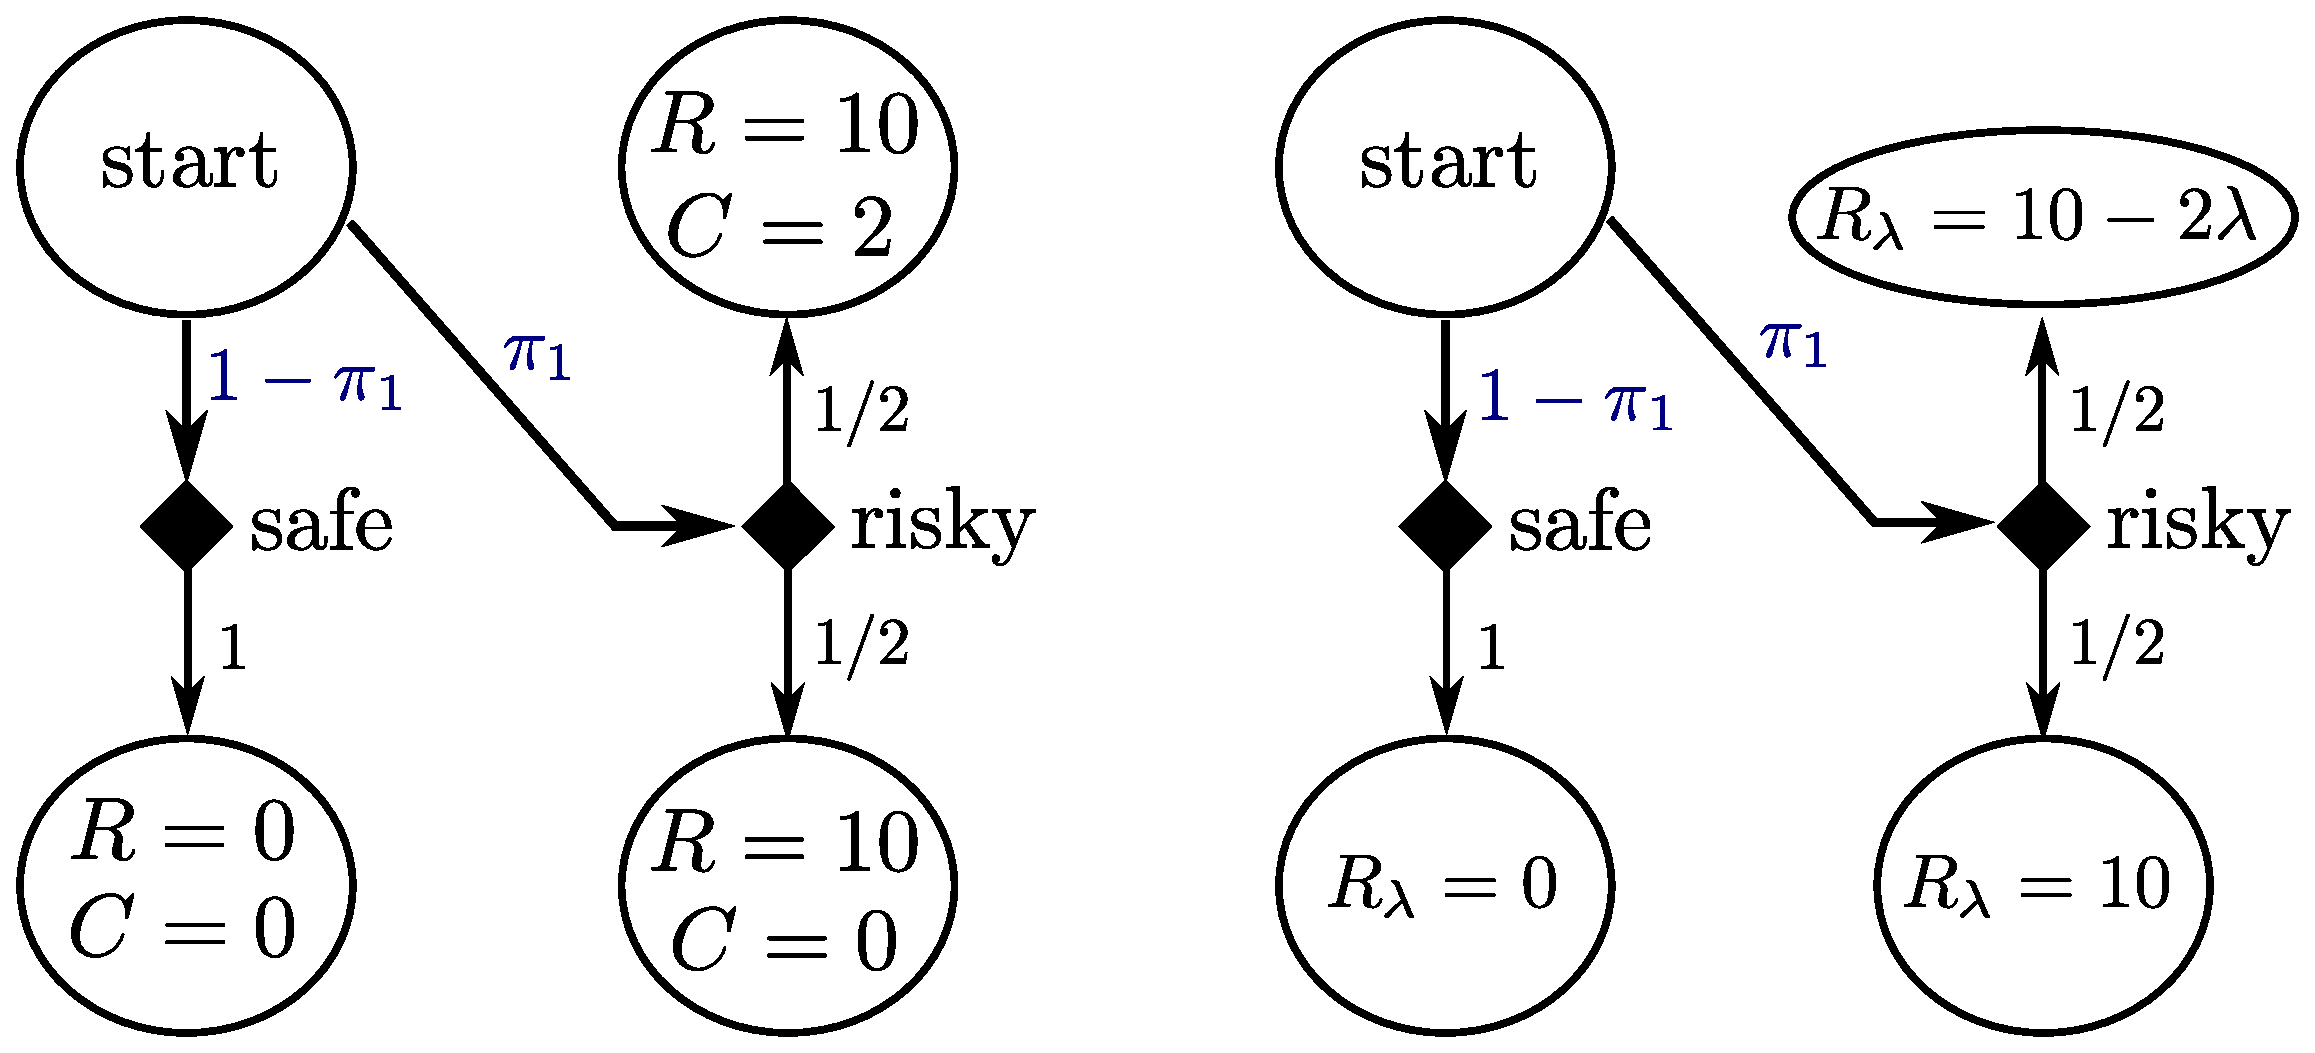
\includegraphics[width=0.6\textwidth]{img/SafeRiskyExample}
	\caption[Example of relaxed Budgeted Markov Decision Process]{On the left hand side, a simple \textit{risky-vs-safe} \gls{BMDP}. The probability of picking the risky action is $\pi_1$. On the right hand side an attempt to relax the problem with negative rewards.}
	\label{fig:stochasticneeded}
\end{figure}

Contrary to \glspl{MDP} which always admit a deterministic optimal policy, this is generally not the case in a \gls{CMDP}, and \textit{a fortiori} in a \gls{BMDP}.
To illustrate this fact, let us consider the trivial \gls{BMDP} on the left of \Cref{fig:stochasticneeded}.
In this example we have $\return^{\policy}=10\pi_1$ and $\constraintreturn[^{\policy}]=\pi_1$. The \idx{deterministic policy} consisting in always picking the safe action is feasible for any $\budget\geq 0$. But if $\budget=1/2$, the most rewarding feasible policy is to randomly pick the safe and risky actions with equal probabilities.
If we attempt to cast this \gls{BMDP} into an \gls{MDP} by replacing the costs by negative rewards, the corresponding greedy policy will be deterministic\index{deterministic policy}, hence sub-optimal.


However, the optimal value function $\oQ^\star$ in a \gls{BMDP} can still be characterised by a fixed-point equation, similarly to \Cref{thm:bellman-optimality-mdp} for \glspl{MDP}.

\begin{theorem}[Budgeted Bellman Optimality]
	\begin{leftbar}[theorembar]
	\label{thm:bellman-optimality}
	The optimal budgeted action-value function $\oQ^{\star}$ verifies
	\begin{equation}
	\label{eq:bellman-optimality}
	\oQ^{\star}(\os, \oa) = \gls+{abo}^{\star}\oQ^{\star}(\os, \oa) \eqdef \gls{oR}(\os, \oa) + \discountfactor \sum_{\os'\in\ocS} \augmentedtransition(\ov{s'} | \os, \oa)\sum_{\ov{a'}\in \ocA} \budgetedpolicy_\text{greedy}(\ov{a'}|\ov{s'}; \oQ^{\star}) \oQ^{\star}(\ov{s'}, \ov{a'}),
	\end{equation}
	where the greedy policy $\budgetedpolicy_\text{greedy}$ is defined by: $\forall \os=(s,\budget)\in \ocS, \oa\in
	\ocA, \forall \oQ\in(\Real^2)^{\ocA\times\ocS},$
	\begin{subequations}
		\label{eq:pi_greedy}
		\begin{align}
		\budgetedpolicy_\text{greedy}(\oa|\os; \oQ) \in &\argmin_{\rho\in\policies_r^{\oQ}} \expectedvalueover{\oa\sim\rho}\Qc(\os, \oa), \label{eq:pi_greedy_cost}\\
		\text{where }\quad\policies_r^{\oQ} \eqdef &\argmax_{\rho\in\cM(\ocA)} \expectedvalueover{\oa\sim\rho} \Qr(\os, \oa) \label{eq:pi_greedy_reward}\\
		& \text{ s.t. }  \expectedvalueover{\oa\sim\rho} \Qc(\os, \oa) \leq \budget. \label{eq:pi_greedy_constraint}
		\end{align}
	\end{subequations}
	\end{leftbar}
\end{theorem}
\begin{proof}
	We provide the proof in \Cref{sec:proof-bell-optim}.
\end{proof}

\begin{remark}[Appearance of the greedy policy]
	\begin{leftbar}[remarkbar]
	\label{rmk:greedy}
	In classical \glsxtrlong{RL}, the greedy policy takes a simple form $\policy_\text{greedy}(s; \Q^{\star}) = \argmax_{a\in\cA} \Q^{\star}(s, a)$, and the term $\policy_\text{greedy}(a'|s';\Q^{\star}) \Q^{\star}(s', a')$ in \eqref{eq:bellman-optimality} conveniently simplifies to $\max_{a'\in \cA} \Q^{\star}(s', a')$. Unfortunately, in a budgeted setting the greedy policy requires solving the nested constrained optimisation program \eqref{eq:pi_greedy} at each state and budget in order to apply this Budgeted Bellman Optimality operator.
	\end{leftbar}
\end{remark}

\begin{proposition}[Optimality of the greedy policy]
	\begin{leftbar}[propositionbar]
	\label{prop:greedy_optimal}
	The greedy policy $\budgetedpolicy_\text{greedy}(\cdot~; \oQ^{\star})$ is {uniformly} optimal: 
	\begin{equation*}
	\text{for all }\os\in\ocS,\,\budgetedpolicy_\text{greedy}(\cdot~; \oQ^{\star})\in\policies^{\star}(\os). 
	\end{equation*}
	In particular, 
	$$\oV^{\budgetedpolicy_\text{greedy}(\cdot; \oQ^{\star})} = \oV^{\star} \text{ and } \oQ^{\budgetedpolicy_\text{greedy}(\cdot; \oQ^{\star})}= \oQ^{\star}.$$
	\end{leftbar}
\end{proposition}
\begin{proof}
	We provide the proof in \Cref{sec:proof-greedy-optim}.
\end{proof}

\paragraph{Budgeted Value Iteration}


\begin{algorithm}
	\DontPrintSemicolon
	\KwData{$P, R_r, R_c$}
	\KwResult{$Q^{\star}$}
	$Q_{0} \leftarrow 0$\;
	\Repeat{convergence ($\|Q_{k+1} - Q_k\|_\infty \leq \epsilon$)}{
		$Q_{k+1} \leftarrow \cT Q_k$\;
	}
	\caption{Budgeted Value Iteration}
	\label{alg:bvi}
\end{algorithm}

The Budgeted Bellman Optimality equation is a fixed-point equation, which motivates the introduction of a fixed-point iteration procedure. We introduce \Cref{alg:bvi}, a \glsxtrlong{DP} algorithm for solving known \glspl{BMDP}. If it were to converge to a unique fixed point, this algorithm would provide a way to compute $\oQ^{\star}$ and recover the associated optimal budgeted policy $\budgetedpolicy_\text{greedy}(\cdot~; \oQ^{\star})$.

\begin{theorem}[Non-contractivity of $\abo^{\star}$]
	\begin{leftbar}[theorembar]
	\label{thm:contraction}
	For any \gls{BMDP} ($\cS,\cA,\Ps,\R,\constraint,\discountfactor$) with $|\cA| \geq 2$, $\abo^{\star}$ is \emph{not} a contraction. Precisely, $$\forall\epsilon>0, \exists \oQ[^1],\,\oQ[^2]\in(\Real^2)^{\ocS\ocA}:\|\abo \oQ[^1]-\abo \oQ[^2]\|_\infty \geq \frac{1}{\epsilon}\|\oQ[^1] - \oQ[^2]\|_\infty.$$
	\end{leftbar}
\end{theorem}
\begin{proof}
	We provide the proof in \Cref{sec:proof-contraction}.
\end{proof}

Unfortunately, as $\abo^{\star}$ is not a contraction, we can guarantee neither the convergence of \Cref{alg:bvi} nor the unicity of its fixed points. Despite those theoretical limitations, we empirically observed the convergence to a fixed point in our experiments (\Cref{sec:brl-experiments}). We provide a possible explanation:

\begin{theorem}[Contractivity of $\cT$ on smooth $Q$-functions]
	\begin{leftbar}[theorembar]
	\label{thm:contractivity-smooth}
	The operator $\abo^{\star}$ is a contraction when restricted to the subset $\cL_{\discountfactor}$ of $\oQ$-functions such that \enquote{$\Qr$ is Lipschitz with respect to $\Qc$}:
	\begin{equation}
	\cL_\discount = \left\{\begin{array}{cc}
	\oQ\in(\Real^2)^{\ocS\ocA}\text{ s.t. }\exists L<\frac{1}{\discount}-1: \forall \os\in\ocS,\oa_1,\oa_2\in\ocA,   \\
	|\Qr(\os,\oa_1) - \Qr(\os,\oa_2)| \leq L|\Qc(\os,\oa_1) - \Qc(\os,\oa_2)|
	\end{array}\right\},
	\end{equation}
	\begin{equation*}
	\forall \oQ[^1],\oQ[^2]\in \cL_\discount,\; \|\abo \oQ[^1]- \abo \oQ[^2]\|_\infty  < \|\oQ[^1]-\oQ[^2]\|_\infty.
	\end{equation*}
	\end{leftbar}
\end{theorem}
\begin{proof}
	We provide the proof in \Cref{sec:contraction-with-smooth}.
\end{proof}

Thus, we expect that \Cref{alg:bvi} is likely to converge when $\oQ^{\star}$ is smooth, but could diverge if the slope of $\oQ^{\star}$ is too high.  $L^2$-regularisation can be used to encourage smoothness and mitigate the risk of divergence.


\section{Budgeted reinforcement learning}

\label{sec:brl}

In this section, we consider \glspl{BMDP} with unknown parameters that must be solved by interaction with an environment. 

\subsection{Budgeted Fitted-Q}
\label{subsec:bftq}

When the \gls{BMDP} is unknown, we need to adapt \Cref{alg:bvi} to work with a batch of samples $\cD=\{(\os_t,\oa_t,\overline{r}_t,\os_t')\}_{t\in [1,N]}$ collected by interaction with the environment. Applying $\abo^{\star}$ in \eqref{eq:bellman-optimality} would require computing an expectation $\expectedvalue_{\os'\sim \augmentedtransition}$ over next states $\os'$ and hence an access to the model $\augmentedtransition$. We instead use $\hat{\abo^{\star}}$, a sampling operator, in which this expectation is replaced by
\begin{equation*}
\hat{\abo^{\star}} \oQ(\os, \oa, \overline{r}, \os') \eqdef \overline{r} + \discount \sum_{\ov{a'}\in \ocA} \pi_\text{greedy}(\ov{a'}|\ov{s'}; \oQ) \oQ(\ov{s'}, \ov{a'}).
\end{equation*}
We introduce in \Cref{alg:bftq} the \gls{BFTQ} algorithm, an extension of the \gls{FTQ} algorithm adapted to solve unknown \glspl{BMDP}. Because we work with continuous state space $\cS$ and budget space $\budgetspace$, we need to employ function-approximation in order to generalise to nearby states and budgets. Precisely, given a parametrized model $\oQ_\params$, we seek to minimise a regression loss $\cL(\oQ_\params, \oQ_\text{target};\cD) = \sum_{\cD} \|\oQ_\params(\os, \oa) - \oQ_\text{target}(\os, \oa, r, \os')\|_2^2$.
Any model can be used, such as linear models, regression trees, or \glsxtrlongpl{NN}.

\begin{algorithm}[ht]
	\DontPrintSemicolon
	\KwData{$\cD$}
	\KwResult{$Q^{\star}$}
	$\oQ_{\params_0} \leftarrow 0$\;
	\Repeat{convergence ($\|Q_{\params_{k+1}} - Q_{\params_{k}}\|_\infty \leq \epsilon$)}{
		$\params_{k+1} \leftarrow \argmin_\params \cL(\oQ_\params, \hat{\cT} \oQ_{\params_{k}}; \cD)$\;
	}
	\caption{Budgeted Fitted-Q}
	\label{alg:bftq}
\end{algorithm}

\subsection{Risk-sensitive exploration}
\label{sec:exploration}

In order to run \Cref{alg:bftq}, we must first gather a batch of samples $\mathcal{D}$. The following strategy is motivated by the intuition that a wide variety of risk levels needs to be experienced during training, which can be achieved by enforcing the risk constraints during data collection. Ideally, we would need samples from the asymptotic state-budget distribution $\lim_{t\rightarrow\infty}\probability{\os_t}$ induced by an optimal policy $\optimalbudgetedpolicy$ given an initial distribution $\probability{\os_0}$, but as we are actually building this policy, it is not possible. Following the same idea of $\epsilon$-greedy exploration for \FTQ, we introduce an algorithm for risk-sensitive exploration. We follow an exploration policy: a mixture between a random \idx{budgeted policy} $\budgetedpolicy_\text{rand}$ and the current greedy policy $\budgetedpolicy_\text{greedy}$. The batch $\cD$ is split into several minibatches generated sequentially, and $\budgetedpolicy_\text{greedy}$ is updated by running \Cref{alg:bftq} on $\cD$ upon mini-batch completion. $\budgetedpolicy_\text{rand}$ is designed to obtain trajectories that only explore feasible budgets: we impose that the joint distribution $\probability{a, \budgetaction|s, \budget}$ verifies $\expectedvalue[\budgetaction]\leq\budget$. This condition defines a probability simplex $\Delta_{\ocA}$ from which we sample uniformly. Finally, when interacting with an environment, the initial state $s_0$ is usually sampled from a starting distribution $\probability{s_0}$. In the budgeted setting, we also need to sample the initial budget $\budget_0$. Importantly, we pick a uniform distribution $\probability{\budget_0} = \gls+{uniform}(\budgetspace)$ so that the entire range of risk-level is explored, and not only reward-seeking behaviours as would be the case with a traditional \idx{risk-neutral} $\epsilon$-greedy strategy. The pseudo-code of our exploration procedure is shown in \Cref{alg:risk-sensitive-exploration}.% in \Cref{sec:risk-sensitive-supp}.

%\section{Risk-Sensitive Exploration}
%\label{sec:risk-sensitive-supp}
%We recall the Risk-Sensitive Exploration in \Cref{alg:risk-sensitive-exploration}:


\begin{algorithm}[ht]
\DontPrintSemicolon
\KwData{An environment, a BFTQ solver, $W$ CPU workers}
\KwResult{A batch of transitions $\cD$}
$\cD\leftarrow\emptyset$\;
\For{each intermediate batch} {
split episodes between $W$ workers\;
\For(\tcp*[f]{run this loop on each worker in parallel}){each episode in batch}{
sample initial budget $\beta\sim\mathcal{U}(\mathcal{B})$.\;
\While{episode not done}{
update $\epsilon$ from schedule.\;
sample $z\sim\mathcal{U}([0, 1])$.\;
\lIf{$z < \epsilon$}{sample $(a, \beta_a)\sim\mathcal{U}(\Delta_{\cA\cB})$.\tcp*[f]{Explore}}
\lElse{sample $(a, \beta_a)\sim\pi_\text{greedy}(a, \beta_a|s, \beta; Q^{\star})$.\tcp*[f]{Exploit}}
append transition $(s, \beta, a, \beta_a, R, C, s')$ to batch $\mathcal{D}$.\;
step episode budget $\beta \leftarrow \beta_a$
}
}
$\pi_\text{greedy}(\cdot\sim; ~Q^{\star}) \leftarrow\texttt{BFTQ}(\cD)$.
}
\Return{the batch of transitions $\cD$}
\caption{Risk-sensitive exploration}
\label{algo:risk-sensitive-exploration}
\end{algorithm}


%\section{A scalable implementation}
%\label{sec:scalable-bftq}
In the following, we introduce an implementation of the \BFTQ algorithm designed to operate efficiently and handle large batches of experiences $\cD$.

\subsection{How to compute the greedy policy?}
\label{subsec:compute-greedy-policy}
As stated in \Cref{rmk:greedy}, computing the greedy policy $\budgetedpolicy_\text{greedy}$ in \eqref{eq:bellman-optimality} is not trivial since it requires solving the nested constrained optimisation program \eqref{eq:pi_greedy}.
However, it can be solved efficiently by exploiting the \emph{structure} of the set of solutions with respect to $\budget$, that is, concave and increasing.

\begin{proposition}[Equality of $\budgetedpolicy_\text{greedy}$ and $\budgetedpolicy_\text{hull}$]
	\begin{leftbar}[propositionbar]
	\label{prop:bftq_pi_hull}
	The greedy policy $\budgetedpolicy_\text{greedy}$ is equal to a convex-hull policy $\budgetedpolicy_\text{hull}$ defined in \Cref{alg:pi_hull}:
    \begin{equation*}
        \budgetedpolicy_\text{greedy}(\oa|\os; \oQ) = \budgetedpolicy_\text{hull}(\oa|\os; \oQ).
    \end{equation*}
    Thus, \Cref{alg:bvi} and \Cref{alg:bftq} can be run by replacing $\budgetedpolicy_\text{greedy}$ in the equation \eqref{eq:bellman-optimality} of $\abo$ with $\budgetedpolicy_\text{hull}$.
    \end{leftbar}
\end{proposition}
\begin{proof}
	We provide the proof in \Cref{sec:proof_pi_hull}.
\end{proof}

\begin{algorithm}[th]
	\DontPrintSemicolon
    \KwData{$\os=(s,\budget)$, $\oQ$}
    $\oQ^+\leftarrow \{\Qc > \min \{\Qc(\os,\oa) \text{ s.t. }\oa\in\argmax_{\oa} \Qr(\os,\oa)\} \}$\tcp*[f]{dominated points}\;
    $\cF \leftarrow \text{top frontier of }\texttt{convex\_hull}(\oQ(\os,\ocA) \setminus \oQ^+)$\tcp*[f]{candidate mixtures}\;
    $\cF_{\oQ} \leftarrow \cF\cap \oQ(\os,\ocA)$\;
    \For{points $q = \oQ(\os,\oa)\in\cF_{\oQ}$ in clockwise order}{
    \uIf{find two successive points $((q_c^1, q_r^1), (q_c^2, q_r^2))$ of $\cF_{\oQ}$ such that $q_c^1 \leq \budget < q_c^2$}{
    $p \leftarrow (\budget - q_c^1) / (q_c^2 - q_c^1)$\;
    \Return the mixture $(1-p)\dirac(\oa-\oa^1) + p\dirac(\oa-\oa^2)$\;
    }}
    \lElse{\Return $\dirac(\oa - \argmax_{\oa} \Qr(\os,\oa))$\tcp*[f]{budget $\budget$ always respected}}
    \caption{Convex hull policy $\budgetedpolicy_\text{hull}(\oa|\os; \oQ)$}
    \label{alg:pi_hull}
\end{algorithm}

\begin{figure}[t]
	\centering
	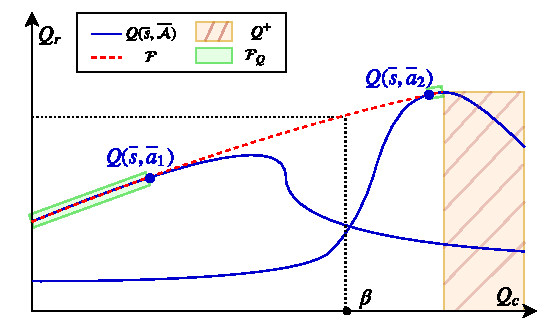
\includegraphics[width=0.6\linewidth]{img/pi.pdf}
	\caption{Representation of $\pi_\text{hull}$. When the budget lies between $Q(\os,\oa_1)$ and $Q(\os,\oa_2)$, two points of the top frontier of the convex hull, then the policy is a mixture of these two points.}
	\label{fig:hull}
\end{figure}

The computation of $\pi_\text{hull}$ in \Cref{alg:pi_hull} is illustrated in \Cref{fig:hull}: first we get rid of dominated points. Then we compute the top frontier of the convex hull of the $Q$-function. Next, we find the two closest augmented actions $\ov{a}_1$ and $\ov{a}_2$ with cost-value $Q_c$ surrounding $\beta$:  $Q_c(\os,\oa_1)\leq\beta<Q_c(\os,\oa_2)$. Finally, we mix the two actions such that the expected spent budget is equal to $\beta$. Because of the concavity of the convex hull top frontier, any other combination of augmented actions would lead to a lower expected reward $Q_r$. 




\subsection{Function approximation}

\glsxtrlongpl{NN} are well suited to model $\oQ$-functions in \gls{RL} algorithms \citep{Mnih2015humanlevel}. We approximate $\oQ = (\Qr, \Qc)$ using one single \glsxtrlong{NN}, as illustrated in \Cref{fig:bftq-architecture}. Thus, the two components are optimised jointly, which accelerates convergence and fosters the learning of useful shared representations. Moreover, as in \citep{Mnih2015humanlevel}, we are dealing with a finite (categorical) action space $\cA$. Instead of including the action in the input, we add an output to the $\oQ$-function for each action. Again, it provides a faster convergence toward useful shared representations and it only requires one forward pass to evaluate all action values. Finally, beside the state $s$ there is one more input to a budgeted $\oQ$-function:~the budget $\budgetaction$. This budget is a scalar value whereas the state $s$ is a vector of potentially large size. To avoid a weak influence of the budget $\budget_a$ compared to the state $s$ in the prediction, we include an additional encoder for the budget, whose width and depth may depend on the application. A straightforward choice is a single layer with the same width as the state.

\subsection{Parallel computing}
\label{subsec:parallel-computing}
In a simulated environment, a first process that can be distributed is the collection of transitions in the exploration procedure of \Cref{alg:risk-sensitive-exploration}, as $\budgetedpolicy_\text{greedy}$ stays constant within each minibatch which avoids the need of synchronisation between workers. Second, the main bottleneck of \gls{BFTQ} is the computation of the target $\abo \oQ$. Indeed, when computing $\budgetedpolicy_\text{hull}$ we must perform at each epoch a Graham-scan of complexity $\cO(|\cA||\tilde{\budgetspace}| \log |\cA||\tilde{\budgetspace}|)$ per transition in $\cD$ to compute the convex hulls of $\oQ$ (where $\tilde{\budgetspace}$ is a finite discretisation of $\budgetspace$). The resulting total time-complexity\footnote{$\log_{\gamma}(\epsilon(1-\gamma))$ is the sample complexity of Value Iteration with accuracy $\epsilon$, and each of these iterations requires a Graham-scan for each state in the dataset $\cD$, action $a\in\cA$ and budget $\beta\in\tilde{\budgetspace}$.} is $\cO(\frac|\cD||\cA||\tilde{\budgetspace}|\log_{\gamma}(\epsilon(1-\gamma)) \log |\cA||\tilde{\budgetspace}|)$. This operation can easily be distributed over several CPUs provided that we first evaluate the model $\oQ(\os',\cA \times \tilde{\budgetspace})$ for each state $\os$ extracted from the dataset $\cD$, which can be done in a single forward pass. By using multiprocessing in the computations of $\budgetedpolicy_\text{hull}$, we enjoy a linear speedup.
The full description of our scalable implementation of \gls{BFTQ} is recalled in \Cref{alg:bftq_full}.


\begin{figure}[tp]
	\centering
	
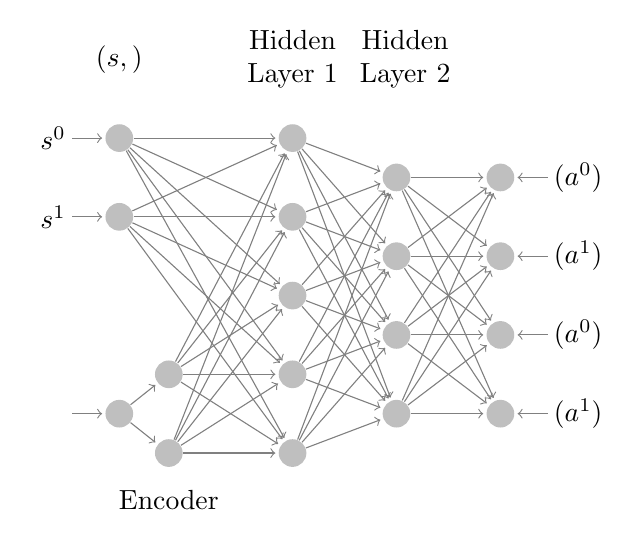
\begin{tikzpicture}[shorten >=1pt,->,draw=black!50, inner sep=1pt, node distance=\layersep]
        \tikzstyle{every pin edge}=[<-,shorten <=1pt]
        \tikzstyle{neuron}=[circle,fill=black!25,minimum size=10pt,inner sep=0pt]
        \tikzstyle{input neuron}=[neuron]
        \tikzstyle{input beta}=[neuron]
        \tikzstyle{qc}=[neuron]
        \tikzstyle{qr}=[neuron]
        \tikzstyle{hidden neuron}=[neuron]
        \tikzstyle{autoencoder neuron}=[neuron]
        \tikzstyle{annot} = [text width=4em, text centered]
        \tikzstyle{annot2} = [text width=10em, text centered]
        \def\layersep{2.2cm}
        % Draw the input layer nodes
        \foreach \name / \y in {0,...,1}
            \pgfmathtruncatemacro{\y}{0 + \y}
            \node[input neuron, pin=left:$s^\y$] (I-\name) at (0,-\y) {};

         % first layer
        \foreach \name / \y in {0,...,4}
        \pgfmathtruncatemacro{\y}{0 + \y}
            \path node[hidden neuron] (H1-\name) at (1*\layersep,-\y cm) {};

        \foreach \source in {0,...,1}
            \foreach \dest in {0,...,4}
                \path (I-\source) edge (H1-\dest);

        % BETA
        \node[input beta, pin=left:$\budgetaction$] (BETA) at (0,-3.5) {};

        % beta auto encoder
        \foreach \name / \y in {0,...,1}
            \pgfmathtruncatemacro{\ybis}{3+ \y}
            \path node[autoencoder neuron] (AE-\name) at (\layersep/3.5,-\ybis cm) {};



        \foreach \name / \y in {0,...,3}
        \pgfmathtruncatemacro{\y}{0 + \y}
            \path[yshift=-0.5cm]
            node[hidden neuron] (H2-\name) at (1.6*\layersep,-\y cm) {};


        % actions
        \foreach \name / \y in {0,...,1}
        \pgfmathtruncatemacro{\y}{0 + \y}
            \path[yshift=-0.5cm] node[qr,pin=right:$\Qr(a^\y)$] (Qr-\name) at (2.2*\layersep,-\y cm) {};

        \foreach \name / \y in {0,...,1}
        \pgfmathtruncatemacro{\yy}{2 + \y}
            \path[yshift=-0.5cm] node[qc,pin=right:$\Qc(a^\y)$] (Qc-\name) at (2.2*\layersep,-\yy cm) {};

        \foreach \source in {0,...,1}
            \foreach \dest in {0,...,4}
                \path (AE-\source) edge (H1-\dest);



        \foreach \dest in {0,...,1}
            \path (BETA) edge (AE-\dest);

         \foreach \source in {0,...,4}
            \foreach \dest in {0,...,3}
                \path (H1-\source) edge (H2-\dest);

        \foreach \source in {0,...,3}
            \foreach \dest in {0,...,1}
                \path (H2-\source) edge (Qr-\dest);

         \foreach \source in {0,...,3}
            \foreach \dest in {0,...,1}
                \path (H2-\source) edge (Qc-\dest);
        % Annotate the layers
       \node[annot] (input) at (0,1) {$(s,\budgetaction)$};
       \node[annot2] (input) at (\layersep/3.5,-4.6) {Encoder};
       \node[annot](h1) at (\layersep,1) {Hidden Layer 1};
       \node[annot](h2) at(1.65 * \layersep,1) {Hidden Layer 2};
       \node[annot](output) at(2.2* \layersep,1) {$\oQ$};
        %\node[annot,right of=hl] {Output layer};
    \end{tikzpicture}

	\caption{Neural Network for $Q$-functions approximation when $\cS=\Real^2$ and $|\cA| = 2$.}
	\label{fig:bftq-architecture}
\end{figure}

\begin{algorithm}[tp]
\DontPrintSemicolon
\KwData{$\mathcal{D}$, $\tilde{\mathcal{B}}$ a finite subset of $\mathcal{B}$, $\discount$, a model $Q\in (\Real^2)^{S \ocA}$, a regression algorithm \texttt{fit}, a set of CPU workers $W$}
\KwResult{$Q^{\star}$}
$Q \leftarrow 0$\;
$X \leftarrow \{s_i,a_i,\beta_{a_i}\}_{i\in[0, |\cD|]}$\;
$S' \leftarrow \{s_i'\}_{i\in[0, |\cD|]}$\;
\Repeat{convergence}{
   Evaluate $Q(S', \cA, \tilde{\cB})$ in a single forward pass\;
   Split $\mathcal{D}$ among workers: $\mathcal{D} = \cup_{w\in W} \mathcal{D}_w$\;
   \For(\tcp*[f]{Run in parallel}){$w\in W$}{
       \For{$(\boldsymbol{\cdot},\boldsymbol{\cdot},\beta_{a_i},{R_r}_i,{R_c}_i,s'_i) \in \mathcal{D}$} {
           $\cP \leftarrow \{(Q_c(s_i',\cA,\tilde{\cB}), Q_r(s_i',\cA,\tilde{\cB}))\}$\;
           $\cP.\texttt{prune}()$ \tcp*[f]{Remove all dominated points}\;
           $\cH \leftarrow \texttt{convex\_hull}(\cP).\text{vertices}()$\tcp*[f]{in cw order}\;
           $k \leftarrow \min\{k: \beta_i \geq q_c$ with $\left(q_c,q_r\right) = \cH[k]\}$\;
           $q_c^2,q_r^2,q_c^1,q_r^1 \leftarrow \cH[k],\cH[k-1]$\;
           $p \leftarrow (\beta_{a_i} - q_a^1) / (q_c^2 - q_c^1)$\;
           $Y_c^{w,i} \leftarrow {R_c}_i + \discount ((1-p) q_c^1+ p q_c^2)$\;
           $Y_r^{w,i} \leftarrow {R_r}_i + \discount ((1-p) q_r^1+ p q_r^2)$\;
       }
   }
   Join the results: $Y \leftarrow \cup_{w\in W} (Y_c^w, Y_r^w)$\;
   $Q \leftarrow \texttt{fit}(X, Y)$\;
}
\caption{A scalable implementation of \gls{BFTQ}}
\label{alg:bftq_full}
\end{algorithm}


\section{Experiments}
\label{sec:brl-experiments}
There are two hypotheses we want to validate.

\paragraph{Exploration strategies} We claimed in \Cref{sec:exploration} that a \idx{risk-sensitive} exploration was required in the setting of \glspl{BMDP}. We test this hypothesis by confronting our strategy to a classical \idx{risk-neutral} strategy. The latter is chosen to be a \idx{$\epsilon$-greedy} policy slowly transitioning from a random to a greedy policy\footnote{We train this greedy policy using \FTQ.} that aims to maximise $\expectedvalue_{\policy} \return^{\policy}$ regardless of $\expectedvalue_{\policy} \constraintreturn[^{\policy}]$. The quality of the resulting batch $\cD$ is assessed by training a \gls{BFTQ} policy and comparing the resulting performance.

\paragraph{Budgeted algorithms} We compare our \BFTQ algorithm to an \FTQl baseline. This baseline consists in approximating the BMDP by a finite set of CMDPs problems. We solve each of these CMDP using the standard technique of Lagrangian Relaxation: the cost constraint is converted into a soft penalty weighted by a Lagrangian multiplier $\lambda$ in a surrogate reward function: $\max_{\policy} \expectedvalue_{\policy}[\return^{\policy} - \lambda \constraintreturn[^{\policy}]]$.
As shown in \Cref{fig:Lagrangian}, the optimal deterministic policy can be obtained by a line-search on the Lagrange multiplier values $\lambda$.
Then, according to \citet[Theorem 4.4]{Beutler1985}, the optimal policy is a randomised mixture of two deterministic policies: the safest deterministic policy that violates the constraint $\pi_{\lambda-}$ and the most risky feasible policy $\pi_{\lambda+}$.
The resulting \glspl{MDP} can be solved by any RL algorithm, and we chose \FTQ for being closest to \BFTQ.
In our experiments, a single training of \BFTQ corresponds to 10 training runs for \FTQl policies. Each run was repeated $N_{\text{seeds}}$ times. Given the high variance, it requires a lot of simulations to get a proper estimate of the calibration curve. Our purpose is to avoid this calibration phase.

\begin{figure}[tp]
	\centering
	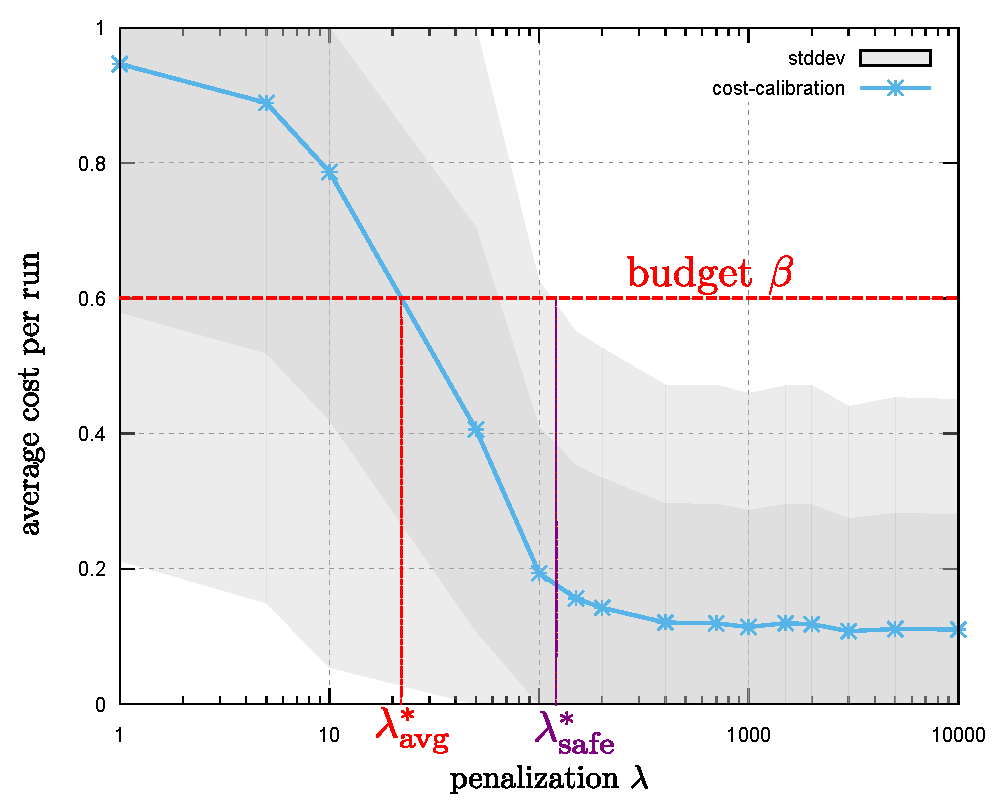
\includegraphics[width=0.5\textwidth]{img/CalibrationExample}
	\caption{Calibration of a penalty multiplier according to the budget $\budget$. The optimal multiplier $\lambda^{\star}_{\text{avg}}$ is the smallest one to satisfy the budget constraint on average. Safer policies can also be selected according to the largest deviation from this mean cost.}
	\label{fig:Lagrangian}
\end{figure}


\subsection{Environments}
\label{subsec:environments}
We evaluate our method on three different environments involving reward-cost trade-offs.

\paragraph{Corridors}
This simple environment is only meant to highlight clearly the specificity of exploration in a budgeted setting. It is a continuous gridworld with Gaussian perturbations, consisting in a maze composed of two corridors: a risky one with high rewards and costs, and a safe one with low rewards and no cost. In both corridors, the outermost cell is the one yielding the most reward, which motivates an in-depth exploration.

\begin{table}[ht!]
    \centering
    \begin{tabular}{lll}
        \toprule
        Parameter & Description & Value\tabularnewline
        \midrule
        - & Size of the environment & 7 x 6\tabularnewline
        - & \makecell[l]{Standard deviation of the Gaussian \\noise applied to actions} & (0.25,0.25)\tabularnewline
        H & Trajectory duration & 9\tabularnewline
        \bottomrule
    \end{tabular}
    \caption{Parameters of \texttt{Corridors}}
    \label{tab:param-corridors}
\end{table}

\paragraph{Spoken dialogue system}
Our second application is a dialogue-based slot-filling simulation that has already benefited from batch RL optimisation in the past~\citep{Li2009ReinforcementLF,chandramohan2010optimizing,pietquin2011sample}. The system fills in a form of slot-values by interacting a user through speech, before sending them a response. For example, in a restaurant reservation domain, it may ask for three slots: the area of the restaurant, the price range and the food type. The user could respectively provide those three slot-values : \texttt{Cambridge}, \texttt{Cheap} and \texttt{Indian-food}. In this application, we do not focus on how to extract such information from the user utterances; but rather on the decision-making for filling in the form. To that end, the system can choose among a set of generic actions. As in \citep{carrara2018safe}, there are two ways of asking for a slot value: a slot value can be either be provided with an utterance, which may cause speech recognition errors with some probability, or by requiring the user to fill in the slots by using a numeric pad. In this case, there are no recognition errors but a counterpart risk of hang-up: we assume that manually filling a key-value form is time-consuming and annoying. The environment yields a reward if all slots are filled without errors, and a constraint if the user hang-ups. Thus, there is a clear trade-off between using utterances and potentially committing a mistake, or using the numeric pad and risking a premature hang-up.

\begin{table}[ht!]
    \centering
    \begin{tabular}{lll}
        \toprule
        Parameter & Description & Value\tabularnewline
        \midrule
        $\xi$ & Sentence Error Rate & 0.6\tabularnewline
        $\mu_{\bot}$& Gaussian mean for misunderstanding & -0.25\tabularnewline
        $\mu_{\top}$& Gaussian mean for understanding & 0.25\tabularnewline
        $\sigma$& Gaussian standard deviation & 0.6\tabularnewline
        $p$& Probability of hang up & 0.25\tabularnewline
        H & Trajectory duration & 10\tabularnewline
        - & Number of slots & 3\tabularnewline
        \bottomrule
    \end{tabular}
    \caption{Parameters of \texttt{Slot-Filling}}
    \label{tab:param-slot-filling}
\end{table}

\paragraph{Two-way road}
In our third application, we use the \highwayenv environment presented in \Cref{chapter:3,chapter:a}.
We define a task that displays a clear trade-off between safety and efficiency, illustrated in \Cref{fig:two-way}. As we mentioned, the agent controls a vehicle with a finite set $\cA$ of manoeuvres \eqref{eq:action-space} implemented by low-level controllers. It is driving on a two-way road populated with other traffic participants: the vehicles in front of the agent drive slowly, and there are incoming vehicles on the opposite lane. The parameters controlling their behaviours are randomised, which introduces some uncertainty concerning their possible future trajectories.
The task consists in driving as fast as possible, which is modelled by a reward proportional to the velocity: $\R(s_t, a_t) \propto v_t$. This motivates the agent to try and overtake its preceding vehicles by driving fast on the opposite lane. This optimal but overly aggressive behaviour can be tempered through a cost function that embodies a safety objective: $\constraint(s_t, a_t)$ is set to $1/H$ whenever the ego-vehicle is driving on the opposite lane, where $H$ is the trajectory horizon. Thus, the constrained signal $\constraintreturn$ is the maximum proportion of time that the agent is allowed to drive on the wrong side of the road.

\begin{figure}[t]
	\centering
	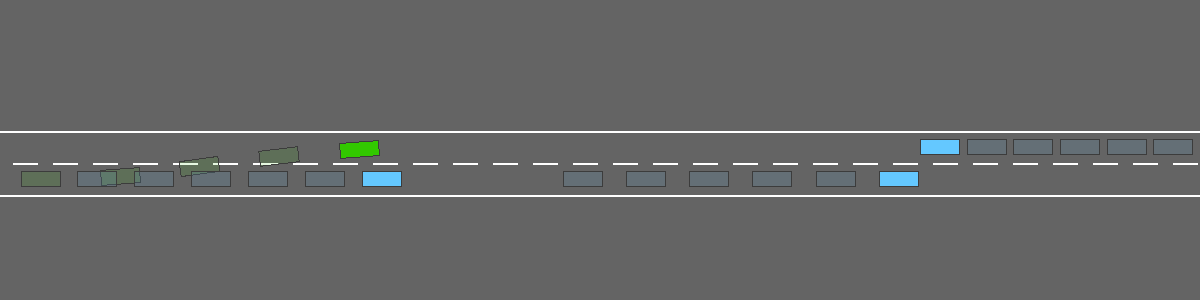
\includegraphics[width=\linewidth]{img/two-way}
	\caption{The two-way road environment requires the vehicle to drive in the wrong lane and risk front collisions in order to overtake slow vehicles.}
	\label{fig:two-way}
\end{figure}

\begin{table}[ht!]
    \centering
    \begin{tabular}{lll}
        \toprule
        Parameter & Description & Value\tabularnewline
        \midrule
        $N_v$& Number of other vehicles & 2 - 6\tabularnewline
        $\sigma_p$& Standard deviation of vehicles initial positions & \SI{100}{\meter}\tabularnewline
        $\sigma_v$& Standard deviation of vehicles initial velocities & \SI{3}{\meter\per\second}\tabularnewline
        H & Trajectory duration & \SI{15}{\second}\tabularnewline
        \bottomrule
    \end{tabular}

    \caption{Parameters of \texttt{highway-env}}
    \label{tab:param-highway-env}
\end{table}

\subsection{Results}
\label{subsec:results}
In the following figures, each patch represents the mean and 95\% confidence interval over $N_{\text{seeds}}$ seeds of the means of $(\return^{\policy},\constraintreturn[^{\policy}])$ ($(\return^{\budgetedpolicy},\constraintreturn[^{\budgetedpolicy}])$ for \BFTQ) over $N_\text{trajs}$ trajectories. That way, we display the variation related to learning (and batches) rather than the variation in the execution of the policies.

We first bring to light the role of risk-sensitive exploration in the \text{corridors} environment. \Cref{fig:exploration-trajs} shows how the two strategies behave in the corridor environment: the risk-neutral procedure focuses on high-reward corridor only, while the risk-sensitive procedure also explores low-risk trajectories. Videos showing the data collection process are available\footnote{\href{https://budgeted-rl.github.io/\#risk-sensitive-exploration}{https://budgeted-rl.github.io/\#risk-sensitive-exploration}}. In \Cref{fig:exploration-perfs}, we observe that this better distributed exploration translates as a uniformly better performance across the range $\budgetspace$ of risk budgets. 
When the budget is low, the corresponding optimal budgeted policy $\budgetedpolicy^\star$ takes the safest path on the left. When the budget increases, it gradually switches to the other lane, earning higher rewards but also costs. This gradual process could not be achieved with a deterministic policy as it would choose either one path or the other. Videos illustrating these optimal policies for different level of risks are available \footnote{\href{https://budgeted-rl.github.io/\#optimal-budgeted-policies-learnt-with-a-risk-sensitive-exploration}{https://budgeted-rl.github.io/\#optimal-budgeted-policies-learnt-with-a-risk-sensitive-exploration}}.

\begin{figure}[th]
	\centering
	\begin{subfigure}[t]{0.48\linewidth}
		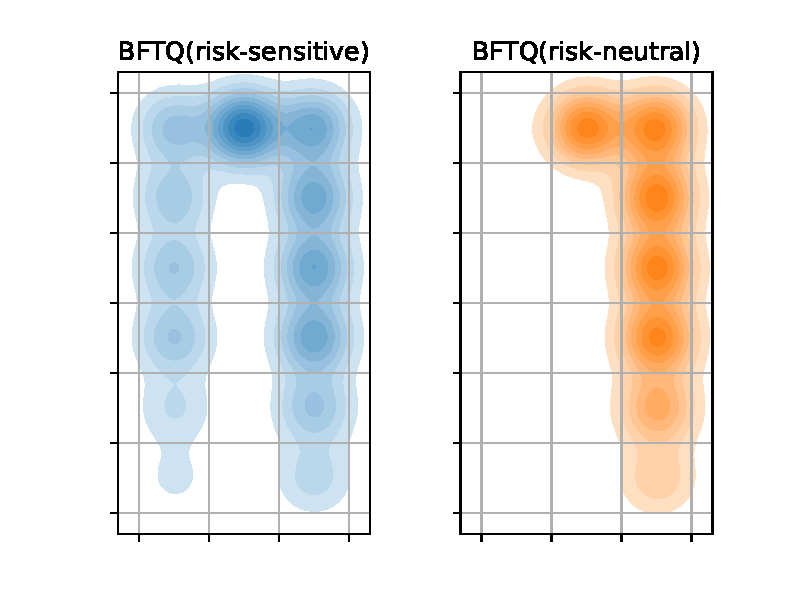
\includegraphics[width=\linewidth]{img/corridors_densities.pdf}
		\caption{State occupations for the two strategies. \emph{Left}: in the \hlb{risk-sensitive} batch, trajectories are well-distributed among both corridors. \emph{Right}: conversely, in the \hlo{risk-neutral} batch, trajectories focus on the risky corridor (to the right) only and ignore the safe corridor (to the left).}
		\label{fig:exploration-trajs}
	\end{subfigure}\hfill
	\begin{subfigure}[t]{0.48\linewidth}
	    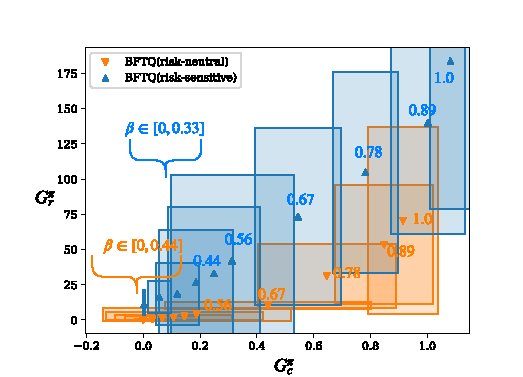
\includegraphics[page=1, width=\textwidth]{img/corridors}
	    \caption{Performances of the optimal budgeted policy $\budgetedpolicy^\star$ trained on batches of transitions obtained by following a \hlo{risk-neutral} and a \hlb{risk-sensitive} exploration. The risk-sensitive procedure attains a better performance across the whole spectrum of risk budgets.}
	    \label{fig:exploration-perfs}
	\end{subfigure}
	\caption{Comparison of two exploration strategies in the corridors environment. }
	\label{fig:exploration}
\end{figure}


\begin{figure}[th]
	\begin{center}
		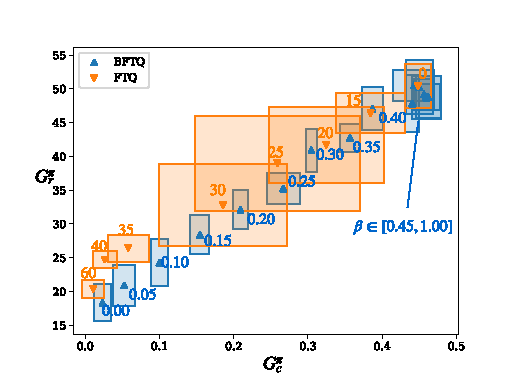
\includegraphics[width=0.49\linewidth]{img/slot-filling}
		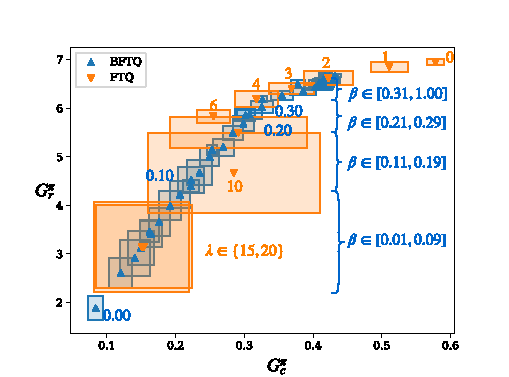
\includegraphics[width=0.49\linewidth]{img/highway}
		\caption{Performance comparison of \FTQl and \BFTQ on \text{slot-filling} (left) and \text{highway-env}(right) }
		\label{sec:brl-results}
	\end{center}
\end{figure}

In a second experiment displayed in \Cref{sec:brl-results}, we compare the performance of \FTQl to that of \BFTQ in the dialogue and autonomous driving tasks. 
For each algorithm, we plot the reward-cost trade-off curve. In both cases, \BFTQ performs almost as well as \FTQl despite only requiring a single model. All budgets are well-respected on \text{slot-filling}, but on \text{highway-env} we can observe an underestimation of $Q_c$, since \eg $\expectedvalue[\constraintreturn|\budget=0] \simeq 0.1 $. This underestimation can be a consequence of two approximations: the use of the sampling operator $\hat{\abo}$ instead of the true population operator $\cT$, and the use of the neural network function approximation $\oQ_\params$ instead of $\oQ$.
Still, \BFTQ provides better control over the expected cost of the policy, than \FTQl. Besides, \BFTQ behaves more consistently than \FTQl overall, as shown by its lower extra-seed variance.
Qualitatively, the budgeted agents display a variety of behaviours, shown in several videos\footnote{\href{https://budgeted-rl.github.io/\#driving-styles}{https://budgeted-rl.github.io/\#driving-styles}}. When $\budget = 1$, the ego-vehicle drives in a very aggressive style: it immediately switches to the opposite lane and drives as fast as possible to pass slower vehicles, swiftly changing lanes to avoid incoming traffic. On the contrary, when $\budget = 0$, the ego-vehicle is conservative: it stays on its lane and drives at a low velocity. With intermediate budgets such as $\budget = 0.2$, the agent sometimes decides to overtake its front vehicle but promptly steers back to its original lane afterwards.

\section*{Discussion}

\Cref{alg:bftq} is an algorithm for solving large unknown \glspl{BMDP} with continuous states. To the best of our knowledge, no algorithm in the current literature combines all those features.

Algorithms have been proposed for \glspl{CMDP}, which are less flexible sub-problems of the more general \gls{BMDP}. When the environment parameters ($\Ps$, $\R$, $\constraint$) are known but not tractable, solutions relying on function approximation~\citep{Undurti2011} or approximate linear programming~\citep{Poupart2015} have been proposed. For unknown environments, Online algorithms \citep{Geibel2005, Abe2010,Achiam2017,Chow2018} and a batch algorithm \citep{Thomas2015, Ghavamzadeh2016, Laroche2019,Le2019} can solve large unknown \glspl{CMDP}. Nevertheless, these approaches are limited in that the constraints thresholds are fixed before training and cannot be updated in real-time at policy execution to select the desired level of risk.

\paragraph{Budgeted Markov Decision Processes algorithms}
To our knowledge, there were only two ways of solving a \gls{BMDP}. The first one is to approximate it with a finite set of \glspl{CMDP} (\eg see our \FTQl baseline). As explained on \Cref{fig:Lagrangian}, the optimal \idx{deterministic policy} can be obtained by a line-search on the Lagrange multiplier values $\lambda$. Then, according to \citet[Theorem 4.4]{Beutler1985}, the optimal policy is a randomised mixture of two deterministic policies\index{deterministic policy}: the safest \idx{deterministic policy} that violates the constraint $\policy_{\lambda-}$ and the riskier of the feasible ones $\policy_{\lambda+}$. So \gls{FTQ} can be easily adapted for continuous states \gls{CMDP} and \gls{BMDP} through this methodology, but given the high variance, it requires many simulations to get a proper estimate of the calibration curve. Our solution not only requires one single model but also avoids any supplementary interaction.

The only other existing \gls{BMDP} algorithm, and closest work to ours, is the \gls{DP} algorithm proposed by \citet{Boutilier_Lu:uai16}. However, their work was established for finite state spaces only, and their solution relies heavily on this property. For instance, they enumerate and sort the next states $s'\in\cS$ by their expected value-by-cost, which could not be performed in a continuous state space $\cS$. Moreover, they rely on the knowledge of the model ($\Ps$, $\R$, $\constraint$), and do not address the question of learning from interaction data.


\section*{Chapter Conclusion}
\label{sec:conclusion}
\glsxtrlongpl{BMDP} are a principled framework for safe decision making under uncertainty, which could be beneficial to the diffusion of Reinforcement Learning in industrial applications. They formulate risk as an expected cumulative cost, which can be estimated and controlled in a model-free fashion. However, \glspl{BMDP} could so far only be solved in finite state spaces which limits their interest for \glsxtrlong{AD} applications that require dealing with continuous variables such as vehicle positions. We extend their scope to continuous states by introducing a novel \glsxtrlong{DP} operator, that we build upon to propose a \glsxtrlong{RL} algorithm. In order to scale to large problems, we provide an efficient implementation that exploits the structure of the value function and leverages tools from Deep Distributed \glsxtrlong{RL}. We show that on two simulated tasks our solution performs similarly to a baseline Lagrangian relaxation method while only requiring a single model to train, and relying on an interpretable risk budget $\budget$ instead of the tedious tuning of the penalty $\lambda$.

%
%\clearpage
%\begin{subappendices}
%%!TEX root = ../../PhD_thesis__Edouard_Leurent.tex
\graphicspath{{2-Chapters/5-Chapter/}}

\chapter{Complements on \Cref{chapter:5}}
\section{Proofs}
\label{sec:proofs}
\subsection{Proof of \Cref{prop:bellman-expectation}}
\label{sec:proof-bell-expect}
\begin{proof}
	Thanks to the introduction of the augmented spaces $\ocS, \ocA$ and dynamics $\augmentedtransition$, this proof is the same as that in classical \glspl{MOMDP}.
	\begin{align*}
	\oV^{\budgetedpolicy}(\os) &\eqdef \expectedvalue\left[ \augmentedreturn^{\budgetedpolicy} \condbar \ov{s_0} = \os\right] \\
	&=\sum_{\oa\in\ocA} \probability{\oa_0 = \oa \condbar\ov{s_0} = \os} \expectedvalue\left[ \augmentedreturn^{\budgetedpolicy} \condbar \ov{s_0} = \os, \oa_0 = \oa\right]\\
	&= \sum_{\oa\in\ocA} \budgetedpolicy(\oa | \os) \oQ^{\budgetedpolicy}(\os,\oa).
	\end{align*}
	
	\begin{align*}
	\oQ^{\budgetedpolicy}(\os, \oa) &\eqdef \expectedvalue\left[\sum_{t=0}^\infty \discountfactor^t \augmentedreward(\os_t, \oa_t)\condbar \ov{s_0} = \os, \ov{a_0} = \oa\right] \\
	&= \augmentedreward(\os, \oa) + \sum_{\os'\in\ocS}\probability{\os_1 = \os' \condbar\ov{s_0} = \os, \ov{a_0} = \oa}\cdot \expectedvalue\left[\sum_{t=1}^\infty \discountfactor^t \augmentedreward(\os_t, \oa_t)\condbar \ov{s_1} = \os'\right] \\
	&= \augmentedreward(\os, \oa) + \discountfactor\sum_{\os'\in\ocS}\augmentedtransition\left(\os' \condbar\os, \oa\right) \expectedvalue\left[\sum_{t=0}^\infty \discountfactor^t \augmentedreward(\os_t, \oa_t) \condbar \ov{s_0} = \os'\right] \\
	&= \augmentedreward(\os, \oa) + \discountfactor\sum_{\os'\in\ocS}\augmentedtransition\left(\os' \condbar\os, \oa\right) \oV^{\budgetedpolicy}(\os').
	\end{align*}
	
	\paragraph{Contraction of $\abo^{\budgetedpolicy}$.}
	Let $\budgetedpolicy\in\policies, \oQ_1, \oQ_2\in(\Real^2)^{\ocS\ocA}$.
	\begin{align*}
	\forall \os\in\ocS, \oa\in\ocA,\quad \left|\abo^{\budgetedpolicy} \oQ_1(\os,\oa) - \abo^{\budgetedpolicy} \oQ_2(\os,\oa)\right| &= \left|\discountfactor\expectedvalueover{\substack{\os'\sim\augmentedtransition(\os'|\os,\oa) \\ \oa'\sim\budgetedpolicy(\oa'|\os')}} \oQ_1(\os',\oa') - \oQ_2(\os',\oa')\right|\\
	&\leq \discountfactor\left\|\oQ_1-\oQ_2\right\|_\infty.
	\end{align*}
	Hence, $\left\|\abo^{\budgetedpolicy} \oQ_1 - \abo^{\budgetedpolicy} \oQ_2 \right\|_\infty \leq \discountfactor\left\|\oQ_1-\oQ_2\right\|_\infty$
	
	According to the Banach fixed point theorem \citep{Banach1922}, $\abo^{\budgetedpolicy}$ admits a unique fixed point.
	It can be easily verified that $\oQ^{\budgetedpolicy}$ is indeed this fixed point by combining the two Bellman Expectation equations~\eqref{eq:bellman_expectation}.
	
\end{proof}

\subsection{Proof of \Cref{thm:bellman-optimality}}
\label{sec:proof-bell-optim}

\begin{proof}
    Let $\os, \oa \in \ocA\times\ocS$. For this proof, we consider potentially non-stationary policies $\budgetedpolicy=(\rho, \budgetedpolicy')$, with $\rho\in\cM(\ocA)$, $\budgetedpolicy'\in\cM(\ocA)^\Natural$. The results will apply to the particular case of stationary optimal policies, when they exist.
    \begin{align}
        \Qr[^\star](\os, \oa) &=  \max_{\rho, \budgetedpolicy'} \Qr[^{\rho, \budgetedpolicy'}](\os', \oa') \label{eq:pthm_def}\\
        &= \max_{\rho, \budgetedpolicy'} \reward(s, a) + \discountfactor \sum_{\os'\in\ocS} \augmentedtransition(\os' | \os, \oa) \Vr[^{\rho, \budgetedpolicy'}](\os') \label{eq:pthm_exp}\\
        &= \reward(s, a) + \discountfactor \sum_{\os'\in\ocS}  \augmentedtransition(\os' | \os, \oa) \max_{\rho, \budgetedpolicy'} \sum_{\oa'\in\ocA} \rho(\oa' | \os')\Qr[^{\budgetedpolicy'}](\os', \oa') \label{eq:pthm_marg}\\
        &= \reward(s, a) + \discountfactor \sum_{\os'\in\ocS}  \augmentedtransition(\os' | \os, \oa) \max_\rho\sum_{\oa'\in\ocA}\rho(\oa' | \os')\max_{\budgetedpolicy'\in\policies_a(\os')}\Qr[^{\budgetedpolicy'}](\os', \oa') \label{eq:pthm_max}\\
        &= \reward(s, a) + \discountfactor \sum_{\os'\in\ocS}  \augmentedtransition(\os' | \os, \oa) \max_\rho\expectedvalueover{\oa'\sim\rho}\Qr[^\star](\os', \oa') \label{eq:pthm_marg_def2}
    \end{align}
    where $\budgetedpolicy = (\rho, \budgetedpolicy')\in\policies_a(\os)$ and $\budgetedpolicy'\in\policies_a(\os')$.

    This follows from:
    \begin{enumerate}
        \item[\eqref{eq:pthm_def}.] Definition of $\oQ^{\star}$.
        \item[\eqref{eq:pthm_exp}.] Bellman Expectation expansion from \Cref{prop:bellman-expectation}.
        \item[\eqref{eq:pthm_marg}.] Marginalisation on $\oa'$.
        \item[\eqref{eq:pthm_max}.] \begin{itemize}
            \item Trivially $\max_{\budgetedpolicy'\in\policies_a(\os')} \sum_{\oa'\in\ocA} \cdot \leq \sum_{\oa'\in\ocA} \max_{ \budgetedpolicy'\in\policies_a(\os)} \cdot$.
            \item Let $\ov{\budgetedpolicy}\in\argmax_{\budgetedpolicy'\in\policies_a(\os')} \Qr[^{\budgetedpolicy'}](\os', \oa')$, then:
            \begin{align*}
                \sum_{\oa'\in\ocA}\rho(\oa'|\os')\max_{\budgetedpolicy'\in\policies_a(\os')}\Qr[^{\budgetedpolicy'}](\os', \oa') &= \sum_{\oa'\in\ocA}\rho(\oa'|\os')\Qr[^{\budgetedpolicy'}](\os', \oa') \\
                &\leq  \max_{\budgetedpolicy'\in\policies_a(\os')} \sum_{\oa'\in\ocA}\rho(\oa'|\os')\Qr[^{\budgetedpolicy'}](\os', \oa').
            \end{align*}
        \end{itemize}
        \item[\eqref{eq:pthm_marg_def2}.] Definition of $\oQ^{\star}$.
    \end{enumerate}

    Moreover, the condition $\budgetedpolicy=(\rho, \budgetedpolicy')\in\policies_a(\os)$ gives
    \begin{equation*}
        \expectedvalueover{\oa'\sim\rho} \Qc[^{\star}](\os, \oa) = \expectedvalueover{\oa'\sim\rho} \Qc[^{\budgetedpolicy'}](\os, \oa) = \Vc[^{\budgetedpolicy}](\os) \leq \budget.
    \end{equation*}

    Consequently, $\budgetedpolicy_\text{greedy}(\cdot; \oQ^{\star})$ belongs to the $\argmax$ of \eqref{eq:pthm_marg_def2}, and in particular:
    \begin{equation*}
        \Qr[^{\star}](\os, \oa) = r(\os, \oa) + \discountfactor \sum_{\os'\in\ocS}  P(\os' | \os, \oa) \expectedvalueover{\oa'\sim\budgetedpolicy_\text{greedy}(\os', \oQ^{\star})} \Qr[^{\star}](\os', \oa').
    \end{equation*}

    The same reasoning can be made for $\Qc[^\star]$ by replacing $\max$ operators by $\min$, and $\policies_a$ by $\policies_r$.
\end{proof}


\subsection{Proof of \Cref{prop:greedy_optimal}}
\label{sec:proof-greedy-optim}
\begin{proof}
    Notice from the definitions of $\abo^{\star}$ and $\abo^{\budgetedpolicy}$ in \eqref{eq:bellman-optimality} and \eqref{eq:bellman_expectation_operator} that $\abo^{\star}$ and $\abo^{\budgetedpolicy_\text{greedy}(\cdot;\oQ^{\star})}$ coincide on $\oQ^{\star}$. Moreover, since $\oQ^{\star} = \abo^{\star}\oQ^{\star}$ by \Cref{thm:bellman-optimality}, we have: $\abo^{\budgetedpolicy_\text{greedy}(\cdot;\oQ^{\star})} \oQ^{\star} = \abo^{\star} \oQ^{\star} = \oQ^{\star}$.
    Hence, $\oQ^{\star}$ is a fixed point of $\abo^{\budgetedpolicy_\text{greedy}(\cdot;\oQ^{\star})}$, and by \Cref{prop:bellman-expectation} it must be equal to $\oQ^{\budgetedpolicy_\text{greedy}(\cdot;\oQ^{\star})}$

    To show the same result for $\oV^{\star}$, notice that
    \begin{equation*}
        \oV^{\budgetedpolicy_\text{greedy}(\oQ^{\star})}(\os) = \expectedvalueover{\oa\sim\budgetedpolicy_\text{greedy}(\oQ^{\star})}\oQ^{\budgetedpolicy_\text{greedy}(\oQ^{\star})}(\os,\oa) = \expectedvalueover{\oa\sim\budgetedpolicy_\text{greedy}(\oQ^{\star})}\oQ^{\star}(\os,\oa).
    \end{equation*}
    By applying the definitions of $\oQ^{\star}$ and $\budgetedpolicy_\text{greedy}$, we recover the definition of $\oV^{\star}$.
\end{proof}

\subsection{Proof of \Cref{thm:contraction}}
\label{sec:proof-contraction}
\begin{proof}
	In the trivial case $|\cA| = 1$, there exits only one policy $\budgetedpolicy$ and $\abo = \abo^\budgetedpolicy$, which is a contraction by \Cref{prop:bellman-expectation}.
	
	In the general case $|\cA| \geq 2$, we can build the following counter-example.
	
	Let $(\cS, \cA, P, R_r, R_c)$ be a \gls{BMDP}.
	For any $\epsilon > 0$, we define $\oQ_\epsilon^1$ and $\oQ_\epsilon^2$ as
	\begin{align*}
	\oQ_\epsilon^1(\os,\oa) =
	\begin{cases}
	(0, 0), & \text{if } a = a_0 \\
	\left(\frac{1}{\discount}, \epsilon\right), & \text{if } a \neq a_0
	\end{cases}\\
	\oQ_\epsilon^2(\os,\oa) =
	\begin{cases}
	(0, \epsilon), & \text{if } a = a_0 \\
	\left(\frac{1}{\discount}, 2\epsilon\right), & \text{if } a \neq a_0
	\end{cases}
	\end{align*}
	Then, $\|\oQ_1-\oQ_2\|_\infty = \epsilon$.
	$\oQ_\epsilon^1$ and $\oQ_\epsilon^2$ are represented in \Cref{fig:concavity_example}.
	
	\begin{figure}[tp]
		\centering
		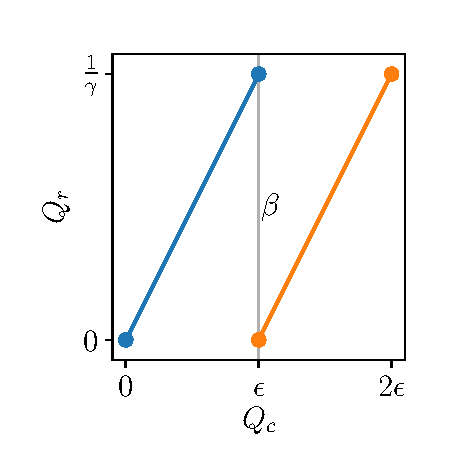
\includegraphics[width=0.4\textwidth]{img/concavity_example.pdf}
		\caption{Representation of $\oQ_\epsilon^1$ (blue) and $\oQ_\epsilon^2$ (yellow)}
		\label{fig:concavity_example}
	\end{figure}
	
	But for $\oa=(a,\budgetaction)$ with $\budgetaction = \epsilon$, we have
	\begin{align*}
	\|\abo \oQ_\epsilon^1(\os, \oa) - \abo \oQ_\epsilon^2(\os, \oa)\|_\infty &= \discount\left\|\expectedvalueover{\os'\sim\augmentedtransition(\os'|\os,\oa)} \expectedvalueover{\oa'\sim\budgetedpolicy_\text{greedy}(\oQ^1_\epsilon)}\oQ^1_\epsilon(\os',\oa') - \expectedvalueover{\oa'\sim\budgetedpolicy_\text{greedy}(\oQ^2_\epsilon)}\oQ^2_\epsilon(\os',\oa')\right\|_\infty \\
	&= \discount\left\|\expectedvalueover{\os'\sim\augmentedtransition(\os'|\os,\oa)}\left(\frac{1}{\discount}, \epsilon\right) - (0, \epsilon)\right\|_\infty \\
	&= \discount\frac{1}{\discount} = 1
	\end{align*}
	Hence, 
	\begin{align*}
	\|\abo \oQ_\epsilon^1 - \abo \oQ_\epsilon^2\|_\infty &\geq 1 = \frac{1}{\epsilon} \|\oQ_1-\oQ_2\|_\infty
	\end{align*}
	
	In particular, there does not exist $L>0$ such that
	$$\forall \oQ_1,\oQ_2\in(\Real^2)^{\ocS\ocA}, \|\abo \oQ^1 - \abo \oQ^2\|_\infty \leq L \|\oQ^1 - \oQ^2\|_\infty$$
	In other words, $\abo$ is not a contraction for $\|\cdot\|_\infty$.
\end{proof}

\subsection{Proof of \Cref{thm:contractivity-smooth}}
\label{sec:contraction-with-smooth}

\begin{remark}
	\begin{leftbar}[remarkbar]
	This proof makes use of insights detailed in the proof of \Cref{prop:bftq_pi_hull} (\Cref{sec:proof_pi_hull}), which we recommend the reader to consult first.
	\end{leftbar}
\end{remark}

\begin{proof}
	We now study the contractivity of $\abo^{\star}$ when restricted to the functions of $\cL_{\discountfactor}$ defined as follows:
    \begin{equation}
    \cL_{\discountfactor} = \left\{\begin{array}{cc}
   \oQ\in(\Real^2)^{\ocS\ocA}\text{ s.t. }\exists L<\frac{1}{\discountfactor}-1: \forall \os\in\ocS,\oa_1,\oa_2\in\ocA,   \\
   |\Qr(\os,\oa_1) - \Qr(\os,\oa_2)| \leq L|\Qc(\os,\oa_1) - \Qc(\os,\oa_2)|
    \end{array}\right\}.
    \end{equation}
    That is, for all state $\os$, the set $\oQ(\os, \ocA)$ plot in the $(\Qc,\Qr)$ plane must be the \emph{graph} of a $L$-Lipschitz function, with $L<1/\discountfactor-1$.

    We impose such structure for the following reason: the counter-example presented above prevented contraction because it was a pathological case in which the slope of $\oQ$ can be arbitrary large. As a consequence, when solving $\Qr[^\star]$ such that $\Qc[^\star]=\budget$, a vertical slice of a $\|\cdot\|_\infty$ ball around $\oQ_1$ (which must contain $\oQ_2$) can be arbitrary large as well.


    We denote $\text{Ball}(\oQ,R)$ the ball of centre $\oQ$ and radius $R$ for the $\|\cdot\|_\infty$-norm:
    \begin{equation*}
        \text{Ball}(\oQ,R) = \{\oQ'\in(R^2)^{\ocS\ocA}: \|\oQ-\oQ'\|_\infty \leq R\}.
    \end{equation*}

    We give the three main steps required to show that $\abo^{\star}$ restricted to $\cL_{\discountfactor}$ is a contraction. Given $\oQ^1, \oQ^2\in\cL_{\discountfactor}$, show that:

    \begin{enumerate}
        \item $\oQ^2\in\text{Ball}(\oQ^1,R)\implies\cF^2\in\text{Ball}(\cF^1, R), \forall\os\in\ocS$, where $\cF$ is the top frontier of the convex hull of undominated points, as defined in~\Cref{sec:proof_pi_hull}.
        \item $\oQ\in\cL_{\discountfactor} \implies \cF$ is the graph of a $L$-Lipschitz function, $\forall\os\in\ocS$.
        \item taking the slice $\Qc=\budget$ of a ball $\text{Ball}(\cF,R)$ with $\cF$ $L$-Lipschitz results in an interval on $\Qr$ of range at most $(L+1)R$
    \end{enumerate}
	
	These three steps will allow us to control $\Qr[^{2\star}] - \Qr[^{1\star}]$ as a function of $R = \|\oQ^2-\oQ^1\|_\infty$.

    \paragraph{Step 1}

    We want to show that if $\oQ^1$ and $\oQ^2$ are close, then $\cF^1$ are $\cF^2$ are close as well in the following sense:
    \begin{align}
        \cF^2\in\text{Ball}(\cF^1, R) &\iff d(\cF^1, \cF^2) \leq R \iff \max_{q^2\in\cF^2}\min_{q^1\in\cF^1}\|q^2-q^1\|_\infty \leq R.
        \label{eq:ball-set}
    \end{align}

    Assume $\oQ^2\in\text{Ball}(\oQ^1,R)$, we show by contradiction that $\cF^2 \in \text{Ball}(\cF^1, R)$. Indeed, assume there exists $q^1\in \cF^1$ such that $\cF^2 \cap \text{Ball}(q^1, R) = \emptyset$. Denote $q^2$ the unique point of $\cF^2$ such that $q^2_c = q^1_c$. By construction of $q^1$, we know that $\|q^1-q^2\|_\infty > R$. There are two possible cases:
    \begin{itemize}
        \item $q^2_r > q^1_r$: this also directly implies that $q^2_r > q^1_r + R$. But $q^2\in\cF^2$, so there exist $q^2_1, q^2_2\in Q^{2},\lambda\in\Real$ such that $q^2 = (1-\lambda)q^2_1 + \lambda q^2_2$. But since $\oQ^2\in \text{Ball}(\oQ^1, R)$, there also exist $q_1^1, q^1_2\in \oQ^1$ such that $\|q^1_1-q^2_1\|_\infty \leq R$ and $\|q^1_2-q^2_2\|_\infty \leq R$, and in particular $q^1_{1r}\geq q^2_{1r}-R$ and $q^1_{2r}\geq q^2_{2r}-R$. But then, the point $q^{1'}=(1-\mu)q^1_1 + \mu q^1_2$ with $\mu=(q^2_c-q^1_{1c})/(q^2_{2c}-q^1_{1c})$ verifies $q^{1'}_c = q^1_c$ and $q^{1'}_r \geq q^2_r - R > q^1_r$ which contradicts the definition of $q_1\in\cF^1$ as defined in \eqref{eq:top-frontier}.
        \item $q^2_r < q^1_r$: then the same reasoning can be applied by simply swapping the indexes 1 and 2.
    \end{itemize}

    % We start by showing this result for $\cC^2(Q^{1-})$ and $\cC^2(Q^{2-})$ as defined in \Cref{sec:proof_pi_hull}:
    % Let $\os\in\ocS$ and $q^2\in\cC^2(Q^{2-})$, $\exists\lambda\in[0,1], \oa_1,\oa_2\in\ocA: q^2 = (1-\lambda)Q^2(\os,\oa_1) + \lambda Q^2(\os,\oa_2)$. Define $q^1 = (1-\lambda)Q^1(\os,\oa_1) + \lambda Q^1(\os,\oa_2)$. Then
    % \begin{align*}
    %     \|q^2-q^1\|_\infty &= \|(1-\lambda)(Q^2(\os,\oa_1) - Q^1(\os,\oa_1)) + \lambda (Q^2(\os,\oa_2) - Q^1(\os,\oa_2))\|_\infty\\
    %     &\leq  (1-\lambda)\|Q^2(\os,\oa_1) - Q^1(\os,\oa_1)\|_\infty + \lambda \|Q^2(\os,\oa_2) - Q^1(\os,\oa_2)\|_\infty\\
    %     &\leq (1-\lambda)R+\lambda R = R
    % \end{align*}

    % It remains to show that when taking the top frontiers of the convex sets $\cC^2(Q^{1-})$ and $\cC^2(Q^{2-})$, they remain at a distance of at most $R$.

    We have shown that $\cF^2 \in \text{Ball}(\cF^1, R)$.
    This is illustrated in \Cref{fig:contraction_lips_hull}: given a function $\oQ^1$, we show the locus $\text{Ball}(\oQ_1,R)$ of $\oQ^2$. We then draw $\cF^1$ the top frontier of the convex hull of $\oQ^1$ and alongside the locus of all possible $\cF^2$, which belong to a ball $\text{Ball}(\cF^1, R)$.

    \begin{figure}[ht]
        \centering
        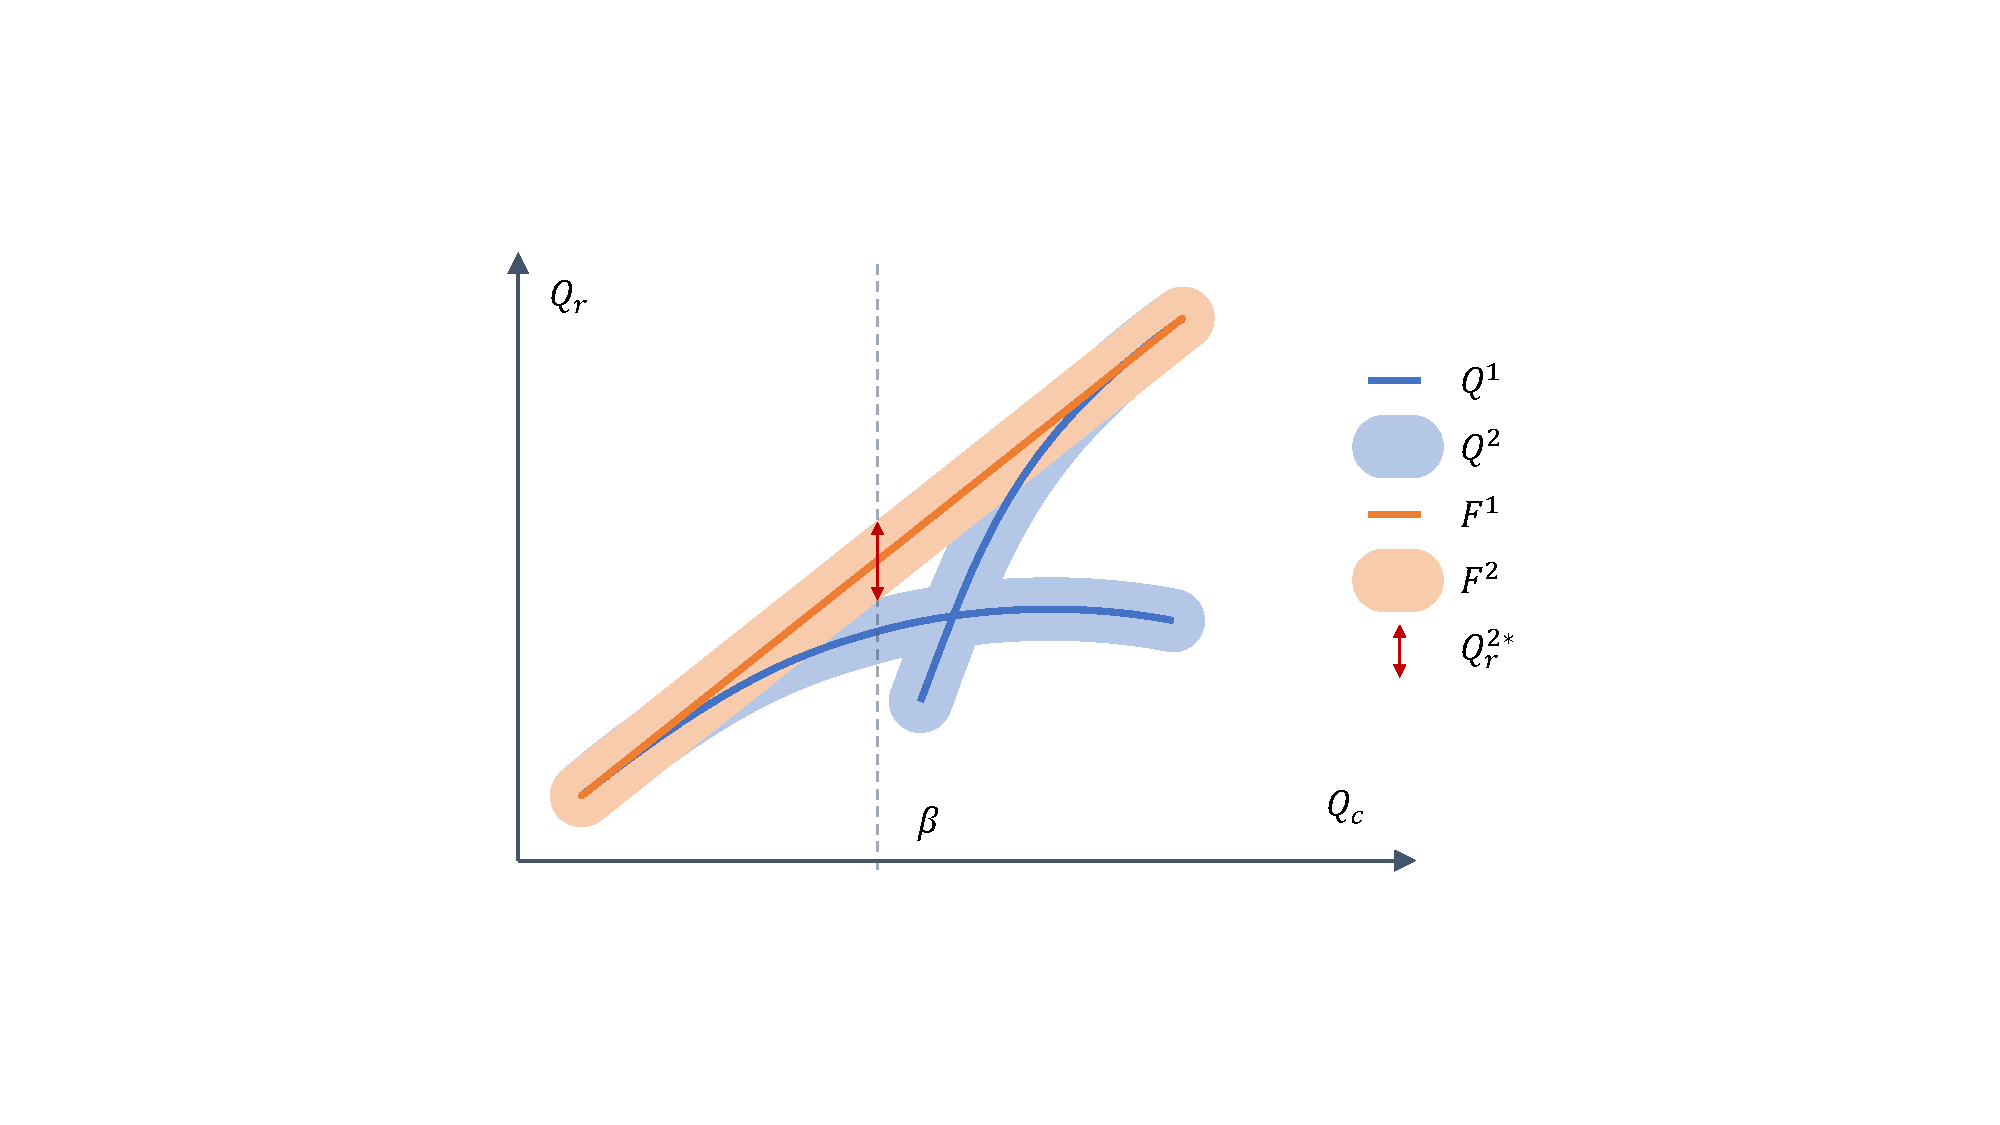
\includegraphics[trim=7cm 4cm 7cm 4cm, clip, width=0.7\textwidth]{img/contraction_lipschitz.pdf}
        \caption{We represent the range of possible solutions $\Qr[^{2\star}]$ for any $\oQ^2\in\text{Ball}(\oQ^1)$, given $\oQ_1\in\cL_\lambda$}
        \label{fig:contraction_lips_hull}
    \end{figure}

    \paragraph{Step 2}

    We want to show that if $\oQ\in\cL_{\discountfactor}$, $\cF$ is the graph of an $L$-Lipschitz function:
    \begin{equation}
        \label{eq:L-lip-set}
        \forall q^1,q^2\in\cF, |q_r^2-q_r^1| \leq |q_c^2-q_c^1|.
    \end{equation}

    Let $\oQ\in\cL_{\discountfactor}$ and $\os\in\ocS$, $\cF$ the corresponding top frontier of convex hull.
    For all $q^1,q^2\in\cF, \exists \lambda,\mu\in[0,1], q^{11},q^{12},q^{21},q^{22}\in \oQ(\os,\ocA)$ such that $q^1 = (1-\lambda)q^{11} + \lambda q^{12}$ and $q^2 = (1-\mu)q^{21} + \mu q^{22}$.
    Without loss of generality, we can assume $q_c^{11}\leq q_c^{12}$ and $q_c^{21}\leq q_c^{22}$. We also consider the worst case in terms of maximum $q_r$ deviation: $q_c^{12} \leq q_c^{21}$.
    Then the maximum increment $q_r^2-q_r^{1}$ is:
    \begin{align*}
        \|q^2_r-q^{1}_r\| &\leq \|q^{12}_r-q^{1}_r\| + \|q^{21}_r-q^{12}_r\| + \|q^{2}_r-q^{21}_r\| \\
        &= (1-\lambda)\|q^{12}_r-q^{11}_r\| + \|q^{21}_r-q^{12}_r\| + \mu\|q^{22}_r-q^{21}_r\| \\
        &\leq (1-\lambda)L\|q^{12}_c-q^{11}_c\| + L\|q^{21}_c-q^{12}_c\| + \mu L\|q^{22}_c-q^{21}_c\| \\
        &= L\|q^{12}_c-q^{1}_c\| + L\|q^{21}_c-q^{12}_c\| + L\|q^{2}_c-q^{21}_c\|\\
        &= L\|q^{2}_c-q^{1}_c\|.
    \end{align*}

    This can also be seen in \Cref{fig:contraction_lips_hull}: the maximum slope of the $\cF^1$ is lower than the maximum slope between two points of $\oQ^1$.

    \paragraph{Step 3}

    Let $\cF_1$ be a L-Lipschitz set as defined in \eqref{eq:L-lip-set}, and consider a ball $\text{Ball}(\cF_1,R)$ around it as defined in \eqref{eq:ball-set}.

    We want to bound the optimal reward value $\Qr[^{2\star}]$ under constraint $\Qc[^{2\star}] = \budget$ (regular case in \Cref{sec:proof_pi_hull} where the constraint is saturated), for any $\cF^2\in\text{Ball}(\cF_1,R)$. This quantity is represented as a red double-ended arrow in \Cref{fig:contraction_lips_hull}.

    Because we are only interested in what happens locally at $\Qc=\budget$, we can zoom in on \Cref{fig:contraction_lips_hull} and only consider a thin $\epsilon$-section around $\budget$. In the limit $\epsilon\rightarrow 0$, this section becomes the tangent to $\cF^1$ at $\Qc[^1]=\budget$. It is represented in \Cref{fig:contraction_lips_hull_slope}, from which we derive a geometrical proof:
    \begin{figure}[ht]
        \centering
        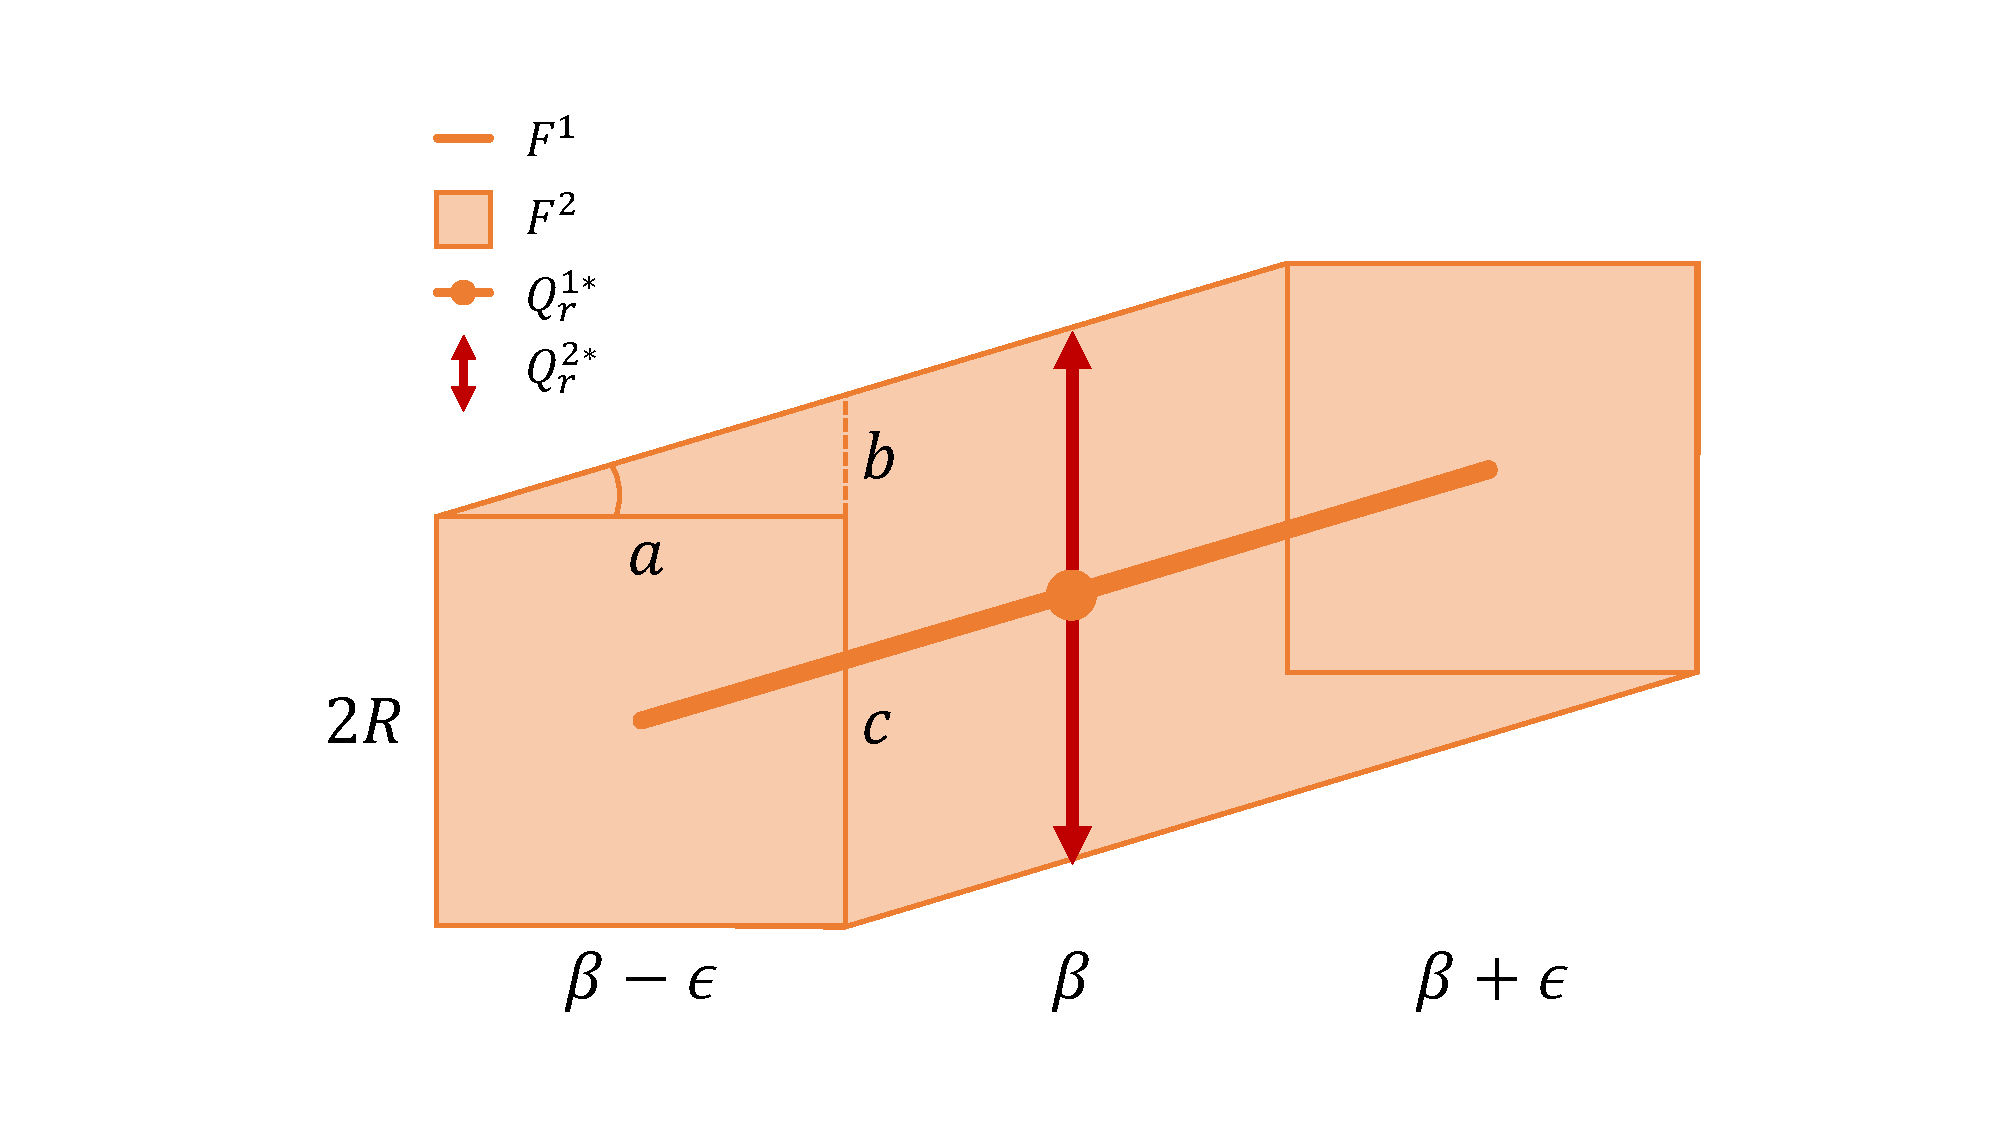
\includegraphics[trim=2cm 1cm 2cm 1cm, clip, width=0.7\textwidth]{img/contraction_lipschitz_slope.pdf}
        \caption{We represent a section $[\budget-\epsilon, \budget+\epsilon]$ of $\cF^1$ and $\text{Ball}(\cF^1, R)$. We want to bound the range of $\Qr[^{2\star}].$}
        \label{fig:contraction_lips_hull_slope}
    \end{figure}
    \begin{align*}
        \Delta \Qr[^{2\star}] &= b + c &\\
        & \leq La + c & \text{($\cF^1$ $L$-Lipschitz)}\\
        &= 2LR+2R = 2R(L+1).
    \end{align*}
    Hence,
    \begin{equation*}
        | \Qr[^{2\star}] - \Qr[^{1\star}]| \leq \frac{\Delta \Qr[^{2\star}]}{2} = R(L+1)
    \end{equation*}
    and $\Qc[^{1\star}] = \Qc[^{2\star}] = \budget$.
    Consequently, $ \|\oQ[^{2\star}] - \oQ[^{1\star}]\|_\infty \leq (L+1)R$.

    Finally, consider the edge case in \Cref{sec:proof_pi_hull}: the constraint is not active, and the optimal value is simply $\argmax_{q\in\cF} q^r$. In particular, since we showed that $\cF^2\in \text{Ball}(\cF^1, R)$, and since $\oQ[^{2\star}]\in \cF^2$, there exist $q^1\in \cF^1: \|\oQ[^{2\star}]-q^1\|_\infty\leq R$ and in particular $\oQ[^{1\star}]_r \geq q^1_r \geq \oQ[^{2\star}]_r - R$. Reciprocally, by the same reasoning, $\Qr[^{2\star}] \geq \Qr[^{1\star}] - R$. Hence, we have that $| \Qr[^{2\star}] - \Qr[^{1\star}]| \leq R \leq R(L+1).$

    \paragraph{Wrapping it up}

    We have shown that for any $\oQ^1,\oQ^2\in\cL_{\discountfactor}$,
    and all $\os\in\ocS$, $\cF^2\in\text{Ball}(\cF^1,\|\oQ^2-\oQ^1\|_\infty)$ and $\cF^1$ is
    the graph of a $L$-Lipschitz function with $L<1/\discountfactor - 1$.
    Moreover, the solutions of $\budgetedpolicy_\text{greedy}(\oQ^1)$ and $\budgetedpolicy_\text{greedy}(\oQ^2)$ at
    $\os$ are such that $ \|\oQ[^{2\star}] - \oQ[^{1\star}]\|_\infty \leq (L+1)\|\oQ^2-\oQ^1\|_\infty$.

    Hence, for all $\oa$,
    \begin{align*}
        \|\abo^{\star}\oQ^1(\os, \oa) - &\abo^{\star}\oQ^2(\os, \oa)\|_\infty \\
        &= \discountfactor\left\|\expectedvalueover{\os'\sim\augmentedtransition(\os'|\os,\oa)}
        \expectedvalueover{\oa'\sim\budgetedpolicy_\text{greedy}(\oQ^1)}\oQ^1(\os',\oa') -
        \expectedvalueover{\oa'\sim\budgetedpolicy_\text{greedy}(\oQ^2)}\oQ^2(\os',\oa')\right\|_\infty \\
        &= \discountfactor\left\|\oQ[^{2\star}] - \oQ[^{1\star}]\right\|_\infty \\
        &\leq \discountfactor(L+1)\|\oQ^2-\oQ^1\|_\infty.
    \end{align*}
    Taking the sup on $\ocS\ocA$,
    \begin{equation*}
        \|\abo^{\star}\oQ^1 - \abo^{\star}\oQ^2\|_\infty \leq \discountfactor(L+1)\|\oQ^1-\oQ^2\|_\infty
    \end{equation*}
    with $\discountfactor(L+1) < 1$.
    As a conclusion, $\abo^{\star}$ is a $\discountfactor(L+1)$-contraction on $\cL_{\discountfactor}$.
\end{proof}

%\subsection{\Cref{lemma:concavity}}

%\begin{proof}. Let $s,s'\in\cS, a\in\cA$.
%We first prove those results for $V_r^{\star}(s', \cdot)$

%\textbf{Non-decreasing}

%Consider $\beta_a^1 \leq \beta_a^2 \in \cB$.
%Any policy that satisfies the budget $\beta_a^1$ in $s'$ also satisfies $\beta_a^2$, so $\Pi_c(s', \beta_a^1) \subset \Pi_c(s', \beta_a^2)$. Hence, by taking the max over policies, $V_r^{\star}(s', \beta_a^1) \leq V_r^{\star}(s', \beta_a^2)$.
%Hence, $V_r^{\star}(s', \cdot)$ is non-decreasing.

%\textbf{Concave}

%By contradiction: assume that $V_r^{\star}(s', \cdot)$ is not concave, \ie there exist $\beta^1 < \beta^2\in \cB$ and $p\in(0, 1)$ such that $\beta^3 = (1-p)\beta^1 + p\beta^2$ verifies: $V_r^{\star}(s', \beta^3) < (1-p)V_r^{\star}(s', \beta^1) + pV_r^{\star}(s',\beta^2)$. By definition of $V^{\star}$, there must be $\pi_1,\pi_2\in\Pi^{\star}$ such that $V^{\star}(s', \beta^1) = V^{\pi_1}(s', \beta^1)$ and $V^{\star}(s', \beta^2) = V^{\pi_2}(s', \beta^2)$. 

%Define $\pi = (1-p)(\pi_1(\cdot, \beta^1), \pi_1) + p(\pi_2(\cdot, \beta^2), \pi_2)$. By linearity of $V^\pi$ with respect to $\pi$, we have that $V_c^\pi(s', \beta^3) = (1-p)V_c^{\pi_1}(s', \beta^1) + pV_c^{\pi_2}(s', \beta^2) \leq (1-p)\beta^1 + p\beta^2 = \beta^3$ since $\pi_1, \pi_2\in\Pi^{\star}(s')\subset\Pi_a(s')$, so $\pi$ respects the budget $\beta^3$. Moreover, we also have $V_r^\pi(s', \beta^3) = (1-p)V_r^{\pi_1}(s', \beta^1) + pV_r^{\pi_2}(s', \beta^2) > V_r^{\star}(s', \beta^3)$, which contradicts the definition of $V_r^{\star}$.

%Consequently, $V_r^{\star}(s', \cdot)$ is non-decreasing and concave. By \eqref{eq:bellman_expectation_Q} we see that $Q_r^{\star}(s,a,\cdot) = R_r(s,a) + \discount\expectedvalueover{s'}V_r^{\star}(s', \cdot)$  is too.


%\end{proof}

%\subsection{\Cref{lemma:tau_concavity}}


%\subsection{\Cref{lemma:pi_hull}}

%\td

%\begin{proof}
%If the estimates $q^c_0, q^c_1$ are accurate, then by construction and linearity of the expectation, the returned mixture policy has an expected total cost of $\expectedvalueover{a, \beta_a \sim\pi_\text{greedy}}Q_c(s, a, \beta_a) = \beta$ as desired in \eqref{eq:pi_greedy_constraint}. Because the $Q_r(s,a,\cdot)$ is concave and under its tangents, this mixture must have the largest $Q_r$ possible as required in \eqref{eq:pi_greedy_reward}. The special case of a tie $q_r^0 = q_r^1$ is considered, where we do minimise $Q_c$ as required in \eqref{eq:pi_greedy_cost}.
%\end{proof}


\subsection{Proof of \Cref{prop:bftq_pi_hull}}
\label{sec:proof_pi_hull}
\begin{definition}
	\begin{leftbar}[defnbar]
	Let $A$ be a set, and $f$ a function defined on $A$. We define
	
	\begin{itemize}
		\item the convex hull of $A$: $\cC(A) = \{\sum_{i=1}^p \lambda_i a_i: a_i\in A, \lambda_i\in\Real^+, \sum_{i=1}^p \lambda_i = 1, p\in\Natural\}$;
		\item the convex edges of $A$: $\cC^2(A) = \{\lambda a_1 + (1-\lambda)a_2: a_1, a_2\in A, \lambda\in[0, 1]\}$;
		\item Dirac distributions of $A$: $\dirac(A) = \{\dirac(a-a_0): a_0\in A\}$;
		\item the image of $A$ by $f$: $f(A) = \{f(a): a\in A\}$.
	\end{itemize}
\end{leftbar}
\end{definition}

\begin{proof}
Let $\os=(s,\budget)\in\ocS$ and $\oQ\in(\Real^2)^{\ocS\ocA}$. We recall the definition of $\budgetedpolicy_\text{greedy}$:
    \begin{subequations}
        \begin{align}
            \budgetedpolicy_\text{greedy}(\oa|\os; \oQ) &\in \argmin_{\rho\in\policies_r^{\oQ}} \expectedvalueover{\oa\sim\rho}\Qc(\os, \oa) \tag{\ref{eq:pi_greedy_cost}}\\
            \text{where }\quad\policies_r^{\oQ} = &\argmax_{\rho\in\cM(\ocA)} \expectedvalueover{\oa\sim\rho} \Qr(\os, \oa) \tag{\ref{eq:pi_greedy_reward}}\\
            & \text{ s.t. }  \expectedvalueover{\oa\sim\rho} \Qc(\os, \oa) \leq \budget \tag{\ref{eq:pi_greedy_constraint}}
        \end{align}
    \end{subequations}

    Note that any policy in the $\argmin$ in \eqref{eq:pi_greedy_cost} is suitable to compute $\abo^{\star}$.
    We first reduce the set of candidate optimal policies.
    Consider the problem described in \eqref{eq:pi_greedy_reward},\eqref{eq:pi_greedy_constraint}: it can be seen as a single-step \gls{CMDP} problem with reward $\reward=\Qr$ and cost $\constraint=\Qc$. By \citep[Theorem 4.4][]{Beutler1985}, we know that the solutions are mixtures of two deterministic policies. Hence, we can replace $\cM(\cA)$ by $\cC^2(\dirac(\ocA))$ in \eqref{eq:pi_greedy_reward}.

    Moreover, remark that:
    \begin{align*}
        \{\expectedvalueover{\oa\sim\rho} \oQ(\os,\oa):& \rho\in \cC^2(\dirac(\ocA))\} \\
        &= \{\expectedvalueover{\oa\sim\rho} \oQ(\os,\oa): \rho=(1-\lambda)\dirac(\oa-\oa_1)+\lambda\dirac(\oa-\oa_2), \oa_1,\oa_2\in\ocA, \lambda\in[0,1]\} \\
        &= \{(1-\lambda)\oQ(\os, \oa_1)+\lambda \oQ(\os, \oa_2), \oa_1,\oa_2\in\ocA, \lambda\in[0,1]\} \\
        &= \cC^2(\oQ(\os,\ocA))\}.
    \end{align*}

    Hence, the problem \eqref{eq:pi_greedy_reward}, \eqref{eq:pi_greedy_constraint} has become:
    \begin{equation*}
        \tilde{\policies}^{\Qr} = \argmax_{(q_r, q_c)\in\cC^2(\oQ(\os, \ocA))} q_r \quad\text{ s.t. }\quad q_c \leq \budget
    \end{equation*}
    and the solution of $\budgetedpolicy_\text{greedy}$ is $q^{\star}=\argmin_{q\in\tilde{\policies}^{\Qr}} q_c$.

    The original problem in the space of actions $\ocA$ is now expressed in the space of values $\oQ(\os, \ocA)$ (which is why we use $=$ instead of $\in$ before $\argmin$ here).

    We further restrict the search space of $q^{\star}$ following two observations:
    \begin{enumerate}
        \item $q^{\star}$ belongs to the \emph{undominated} points $\cC^2(\oQ^-)$:
        \begin{align}
            \label{eq:q_minus_undominated}
            \oQ^+ &= \{(q_c, q_r): q_c > q_c^{\pm} = \min_{q^+} q_c^+\text{ s.t. }q^+\in\argmax_{q\in \oQ(\os,\ocA)} q_r\}\\
            \oQ^- &= \oQ(\os,\ocA) \setminus \oQ^+.
        \end{align}
        Denote $q^{\star}$ = $(1-\lambda) q^1 + \lambda q^2$, with $q^1, q^2\in \oQ(\os,\ocA)$. There are three possible cases:
        \begin{enumerate}
            \item $q^1, q^2 \not\in \oQ^-$. Then $q_c^{\star} = (1-\lambda) q^1_c + \lambda q^2_c > q_c^{\pm}$. But then $q_c^{\pm} < q_c^{\star} \leq \budget$ so $q^{\pm}\in\tilde{\policies}^{\Qr}$ with a strictly lower $q_c$ than $q^{\star}$, which contradicts the $\argmin$.
            \item $q^1\in \oQ^-, q^2 \not\in \oQ^-$. But then consider the mixture $q^\top = (1-\lambda) q^1 + \lambda q^\pm$. Since $q_r^{\pm} \geq q_r^{2}$ and $q_r^{\pm} < q_r^{2}$, we also have $q^\top_r \geq q_r^{\star}$ and $q^\top_c < q_c^{\star}$, which also contradicts the $\argmin$.
            \item $q^1,q^2\in \oQ^-$ is the only remaining possibility.
        \end{enumerate}
        \item $q^{\star}$ belongs to the \emph{top frontier} $\cF$:
        \begin{equation}
            \label{eq:top-frontier}
            \cF_{\oQ} = \{q\in \cC^2(\oQ^-): \not\exists q'\in \cC^2(\oQ^-): q_c=q_c'\text{ and }q_r<q_r'\}.
        \end{equation}
        Trivially, otherwise q' would be a better candidate than $q^{\star}$.
    \end{enumerate}


    Let us characterise this frontier $\cF$. It is both:
    \begin{enumerate}
        \item the \emph{graph of a non-decreasing function}: $\forall q^1, q^2\in\cF$ such that $q_c^1\leq q_c^2$ then $q_r^1\leq q_r^2$.\\
        By contradiction, if we had $q_r^1 > q_r^2$, we could define $q^\top = (1-\lambda)q^1 + \lambda q^\pm$ where $q^\pm$ is the dominant point as defined in \eqref{eq:q_minus_undominated}. By choosing $\lambda=(q^2_c-q^1_c)/(q^\pm_c-q^1_c)$ such that $q^\top_c = q_c^2$, then since $q_r^\pm \geq q_r^1 > q_r 2$ we also have $q^\top_r > q_r^2$ which contradicts $q^2\in\cF$.
        \item the \emph{graph of a concave function}: $\forall q^1, q^2, q^3\in\cF$ such that $q_c^1\leq q_c^2 \leq q_c^3$ with $\lambda$ such that $q^2_c = (1-\lambda)q^1_c + \lambda q^3_c$, then $q_r^2 \geq (1-\lambda)q_r^1 + \lambda q_r^3$.\\
        Trivially, otherwise the point $q^\top = (1-\lambda)q^1 + \lambda q^3$ would verify $q^\top_c=q^2_c$ and $q^\top_r > q^2_r$, which would contradict $q^2 \in\cF$.
    \end{enumerate}

    We denote $\cF_{\oQ} = \cF \cap \oQ$. Clearly, $q^{\star}\in\cC^2(\cF_{\oQ})$: let $q^1, q^2\in \oQ^-$ such that $q^{\star} = (1-\lambda)q^1 + \lambda q^2$. First, $q^1, q^2\in \oQ^-\subset\cC^2(\oQ^-)$. Then, by contradiction, if there existed $q^{1'}$ or $q^{2'}$ with equal $q_c$ and strictly higher $q_r$, again we could build an admissible mixture $q^{\top}=(1-\lambda)q^{1'}  + \lambda q^{2'}$ strictly better than $q^{\star}$.

    $q^{\star}$ can be written as $q^{\star} = (1-\lambda)q^1 + \lambda q^2$ with $q^1, q^2\in\cF_{\oQ}$ and, without loss of generality, $q^1_c \leq q^2_c$.

    \paragraph{Regular case}

    There exists $q^0\in\cF_{\oQ}$ such that $q^0_c \geq \budget$. Then $q^1$ and $q^2$ must flank the budget: $q_c^1 \leq \budget \leq q_c^2$. Indeed, by contradiction, if $q_c^2 \geq q_c^1 > \budget$ then $q_c^{\star} > \budget$ which contradicts $\policies_r^{\oQ}$. Conversely, if $q_c^1 \leq q_c^2 < \budget$ then $q^{\star} < \budget \leq q^0_c$, which would make $q^{\star}$ a worse candidate than $q^\top=(1-\lambda)q^{\star} + \lambda q^0$ when $\lambda$ is chosen such that $q_c^\top=\budget$, and contradict $\policies_r^{\oQ}$ again.

    Because $\cF$ is the graph of a non-decreasing function, $\lambda$ should be as high as possible, as long as the budget $q^{\star}\leq\budget$ is respected. We reach the highest $q_r^{\star}$ when $q^{\star}_c=\budget$, that is: $\lambda=(\budget-q_c^1)/(q_c^2-q_c^1)$.

    It remains to show that $q^1$ and $q^2$ are two successive points in $\cF_{\oQ}$: $\not\exists q\in\cF_{\oQ}\setminus\{q^1, q^2\}: q^1_c \leq q_c \leq q^2_c$. Otherwise, as $\cF$ is the graph of a concave function, we would have $q_r \geq (1-\mu)q_r^1 + \mu q_r^2$. $q_r$ cannot be strictly greater than $(1-\mu)q_r^1 + \mu q_r^2$ which would contradict $q^{\star}$, but it can still be equal, which means the tree points $q, q^1, q^2$ are aligned. In fact, every points aligned with $q^1$ and $q^2$ can also be used to construct mixtures resulting in $q^{\star}$, but among these solutions we can still choose $q^1$ and $q^2$ as the two points in $\cF_{\oQ}$ closest to $q^{\star}$.

    \paragraph{Edge case}

    $\forall q\in\cF_{\oQ}, q_c < \budget$. Then  $q^{\star} =  \argmax_{q\in\cF} q_r = q^\pm =  \argmax_{q\in \oQ^-} q_r$.
\end{proof}


%\begin{proof}
%First, a straightforward proof by induction shows that for all $k\in\Natural$, $Q_k$ computed at iteration $k$ of either \Cref{alg:bvi} or \Cref{alg:bftq} is concave non-decreasing with respect to $\beta_a$: the initialisation is trivial from $Q_0 = 0$, and the heredity stems from \Cref{lemma:tau_concavity}.
%\end{proof}


% \subsection{Decomposition Lemma}

% \begin{lemma}
%     For any sequence real valued functions $f_1,\ldots,f_n$ and any real number $c$, we have
%     \[
%         \begin{array}{lcl}
%             \underbrace{\max\limits_{\sum_i x_i \leq c}\sum_j f_j(x_j)}_{(a)} & \quad{}=\quad{} & \underbrace{\max\limits_{\sum_i c_i \leq c}\left(\sum_j\max\limits_{x\leq c_j} f_j(x)\right)}_{(b)}\\
%         \end{array}
%     \]
% \end{lemma}

% \begin{proof}
%     Let us first show that $(a)\leq(b)$.
%     By definition of the maximum on a set, for any $f_j$ and any $c_j$ we have
%     $\max\limits_{x\leq c_j} f_j(x) \geq f_j(c_j)$.
%     Hence, by replacing these terms in $(b)$ we get:
%       \[
%     \begin{array}{lcl}
%         \max\limits_{\sum_i c_i \leq c} \sum_j f_j(c_j) & \quad{}\leq\quad{} & \max\limits_{\sum_i c_i\leq c}\left(\sum_j \max\limits_{x_j\leq c_j} f_j(x_j)\right)\\
%     \end{array}
%     \]
%     The left hand side of this inequality is just a rewriting of $(a)$ with different dummy variables names.

%     Let us show now that $(a) \geq (b)$.
%     Let $\hat{x}_1,\ldots,\hat{x}_n, \hat{c}_1, \ldots \hat{c}_n$ be a realisation (argmax) of $(b)$.
%     By definition of $(b)$'s feasible set, we have $\sum_i\hat{c}_i \leq c$ and for any $i$: $\hat{x}_i\leq \hat{c}_i$.
%     Because $\sum_i\hat{x}_i\leq \sum_i\hat{c}_i \leq c$, the tuple $(\hat{x}_1, \ldots \hat{x}_n)$ is also a feasible value for $(a)$. And, by definition of the maximum on a set: $(a) = \max\limits_{\sum_i x_i \leq c} \sum_j f_j(x_j) \geq \sum_j f_j(\hat{x}_j) = (b)$.
% \end{proof}

%\section{Risk-Sensitive Exploration}
%\label{sec:risk-sensitive-supp}
%We recall the Risk-Sensitive Exploration in %\Cref{alg:risk-sensitive-exploration}:
%\begin{algorithm}[ht]
\DontPrintSemicolon
\KwData{An environment, a BFTQ solver, $W$ CPU workers}
\KwResult{A batch of transitions $\cD$}
$\cD\leftarrow\emptyset$\;
\For{each intermediate batch} {
split episodes between $W$ workers\;
\For(\tcp*[f]{run this loop on each worker in parallel}){each episode in batch}{
sample initial budget $\beta\sim\mathcal{U}(\mathcal{B})$.\;
\While{episode not done}{
update $\epsilon$ from schedule.\;
sample $z\sim\mathcal{U}([0, 1])$.\;
\lIf{$z < \epsilon$}{sample $(a, \beta_a)\sim\mathcal{U}(\Delta_{\cA\cB})$.\tcp*[f]{Explore}}
\lElse{sample $(a, \beta_a)\sim\pi_\text{greedy}(a, \beta_a|s, \beta; Q^{\star})$.\tcp*[f]{Exploit}}
append transition $(s, \beta, a, \beta_a, R, C, s')$ to batch $\mathcal{D}$.\;
step episode budget $\beta \leftarrow \beta_a$
}
}
$\pi_\text{greedy}(\cdot\sim; ~Q^{\star}) \leftarrow\texttt{BFTQ}(\cD)$.
}
\Return{the batch of transitions $\cD$}
\caption{Risk-sensitive exploration}
\label{algo:risk-sensitive-exploration}
\end{algorithm}

%\end{subappendices}


\chapter*{Part Conclusion\\ {\LARGE Review of our Requirements}}
\mtcaddchapter[Part Conclusion]

Let us come back to the specifications of desirable properties for a behavioural planning algorithm, that we advocated in \Cref{chapter:1}. In \Cref{tab:part-2-conclusion}, we examine whether these criteria are met by the methods developed in \Cref{part:2}.

\begin{table}[H]
	\begin{tabularx}{\linewidth}{p{4.3cm}cX}
		\toprule
		Criterion & & Description \\
		\midrule
		\textbf{Social Awareness} & {\Large $\hlgb{\checkmark}$} & In \Cref{chapter:4}, we introduced an attention-based \glsxtrlong{NN} architecture that explicitly attends to other drivers in the scene, sorting out irrelevant vehicles from those that represent a source of danger. \\
		\textbf{Sample Efficiency} & {\Large $\hlgb{\checkmark}$} & We showed in \Cref{fig:attention-reward} that this architecture also comes with an inductive bias -- permutation invariance -- that allows to fasten the training process. \\
		\textbf{Safety} & {\Large $\hlgb{\checkmark}$} & A first notion of risk was introduced in \Cref{chapter:5}, in the shape of a cost signal $\constraint(s,a)$ constrained to remain below a threshold $\budget$, in expectation. This formulation makes it possible to state safety specifications orthogonal to the traditional reward maximisation objective.\\
		\textbf{Balance between safety and efficiency} & {\Large $\hlgb{\checkmark}$} & The cost budget $\budget$ can be adjusted in real time as an input of the budgeted policy $\budgetedpolicy$ to trade-off safety with  efficiency \\
		\bottomrule
	\end{tabularx}
	\caption{Do the methods of \Cref{part:2} comply with the specifications of \Cref{chapter:1}?}
	\label{tab:part-2-conclusion}
\end{table}

\part{Model-based}
\label{part:3}

\vspace*{2cm}
\begin{flushright}
	\begin{tabular}{@{}l@{}}
		\emph{\dots et prévoir en stratège.}\\
	\end{tabular}
	
	René Char, \href{https://eleurent.github.io/sisyphe/texts/feuillets-d-hypnos.html}{\emph{Feuillets d'Hynos}}.
\end{flushright}

%!TEX root = ../../PhD_thesis__Edouard_Leurent.tex

\graphicspath{{2-Chapters/6-Chapter/}}

\chapter{Planning Fast by Hoping for the Best}
\label{chapter:6}

\begin{flushright}
	\begin{tabular}{@{}l@{}}
		\emph{Nous voulons, tant ce feu nous brûle le cerveau,}\\
		\emph{Plonger au fond du gouffre, Enfer ou Ciel, qu’importe ?}\\
		\emph{Au fond de l’Inconnu pour trouver du nouveau !}\\
	\end{tabular}
	
	Charles Baudelaire, \href{https://eleurent.github.io/sisyphe/texts/le-voyage.html}{\emph{Le voyage}}.
\end{flushright}

\abstractStartChapter{}%

In a \emph{Markov Decision Process} (MDP), an agent observes its current state $s$ from a state space $S$ and picks an action $a$ from an action space $A$, before transitioning to a next state $s'$ drawn from a transition kernel $\probability{s'|s,a}$ and receiving a bounded reward $r\in[0, 1]$ drawn from a reward kernel $\probability{r|s, a}$. The agent must act so as to optimise its expected cumulative discounted reward $\expectedvalue \sum_t \gamma^t r_t$, also called expected \emph{return}, where $\gamma\in[0,1)$ is the discount factor. In \emph{Online Planning} \cite{Munos2014}, we do not consider that these transition and reward kernels are known as in \emph{Dynamic Programming} \citep{Bellman1957}, but rather only assume access to the MDP through a \emph{generative model} (e.g. a simulator) which yields samples of the next state $s' \sim \probability{s'|s,a}$ and reward $r\sim\probability{r|s, a}$ when queried. Finally, we consider a \emph{fixed-budget} setting where the generative model can only be called a maximum number of times, called the budget $n$. 

\minitocStartChapter{}

\emph{Monte-Carlo Tree Search} (\texttt{MCTS}) algorithms were historically motivated by the application of computer Go, and made a first appearance in the CrazyStone software \citet{Coulom2006}. They were later reformulated in the setting of Multi-Armed Bandits by \citet{Kocsis2006} with their \emph{Upper Confidence bounds applied to Trees} (\texttt{UCT}) algorithm. Despite its popularity \citep{Silver2016,Silver2017,Silver2018}, \texttt{UCT} has been shown to suffer from several limitations: its sample complexity can be at least doubly-exponential for some problems (e.g. when a narrow optimal path is hidden in a suboptimal branch), which is much worse than uniform planning \citep{Coquelin2007}. The \texttt{Sparse Sampling} algorithm of \citet{Kearns2002} achieves better worst-case performance, but it is still non-polynomial and doesn't adapt to the structure of the MDP. In stark contrast, the \emph{Optimistic Planning for Deterministic systems} (\OPD) algorithm considered by \citet{Hren2008} in the case of deterministic transitions and rewards exploits the structure of the cumulative discounted reward to achieve a problem-dependent polynomial bound on sample complexity. A similar line of work in a deterministic setting is that of \texttt{SOOP} and \texttt{OPC} by \cite{Busoniu2013,Busoniu2018} though they focus on continuous action spaces. \OPD was later extended to stochastic systems with the \emph{Open-Loop Optimistic Planning} (\OLOP) algorithm introduced by \citet{Bubeck2010} in the open-loop setting: we only consider sequences of actions independently of the states that they lead to. This restriction in the space of policies causes a loss of optimality, but greatly simplifies the planning problem in the cases where the state space is large or infinite. More recent work such as \texttt{St0p} \citep{Szorenyi2014} and \texttt{TrailBlazer} \citep{Grill2016} focus on the probably approximately correct (PAC) framework: rather than simply recommending an action to maximise the expected rewards, they return an $\epsilon$-approximation of the value at the root that holds with high probability. This highly demanding framework puts a severe strain on these algorithms that were developed for theoretical analysis only and cannot be applied to real problems.

\section{Open-loop optimistic planning}

\paragraph{Contributions} The goal of this section is to study the practical performances of \OLOP when applied to numerical problems. Indeed, \OLOP was introduced along with a theoretical sample complexity analysis but no experiment was carried-out. Our contribution is threefold:

\begin{itemize}
	\item First, we show that in our experiments \OLOP is overly pessimistic, especially in the low-budget regime, and we provide an intuitive explanation by casting light on an unintended effect that alters the behaviour of \OLOP.
	\item Second, we circumvent this issue by leveraging modern tools from the bandits literature to design and analyse a modified version with tighter upper-confidence bounds called \KLOLOP. We show that we retain the asymptotic regret bounds of $\OLOP$ while improving its performances by an order of magnitude in numerical experiments.
	\item Third, we provide a time and memory efficient implementation of \OLOP and \KLOLOP, bringing an exponential speedup that allows to scale these algorithms to high sample budgets.
\end{itemize}

The paper is structured as follows: in section \ref{sec:kl-olop}, we present \OLOP, give some intuition on its limitations, and introduce \KLOLOP, whose sample complexity is further analysed in section \ref{sec:sample-complexity}. In section \ref{sec:time-complexity}, we propose an efficient implementation of the two algorithms. Finally in section \ref{sec:planning-experiments}, we evaluate them in several numerical experiments.

\paragraph{Notations}
We follow the notations from \citep{Bubeck2010} and use the standard notations over alphabets: a finite word $a \in A^*$ of length $h$ represents a sequence of actions $(a_0, \cdots, a_h) \in A^h$. Its prefix of length $t \leq h$ is denoted $a_{1:t} = (a_0,\cdots,a_t) \in A^t$. $A^\infty$ denotes the set of infinite sequences of actions. Two finite sequences $a\in A^*$ and $b\in A^*$ can be concatenated as $ab\in A^*$, the set of finite and infinite suffixes of $a$ are respectively $a A^* = \{c\in\mathcal{A}^*: \exists b\in A^*$ such that $c=ab\}$ and $aA^\infty$ defined likewise, and the empty sequence is $\emptyset$.

During the planning process, the agent iteratively selects sequences of actions until it reaches the allowed budget of $n$ actions. More precisely, at time $t$ during the $m^{\text{th}}$ sequence, the agent played $a^m_{1:t} = a^m_1 \cdots a^m_t \in A^t$ and receives a reward $Y_t^m$. We denote the probability distribution of this reward as $\nu(a_{1:t}^m) = \probability{Y_t^m | s_t, a^m_t} \prod_{k=1}^{t-1} \probability{s_{k+1} | s_{k}, a_{k}^m}$, and its mean as $\mu(a_{1:t}^m)$, where $s_1$ is the current state.

After this exploration phase, the agent selects an action $a(n)$ so as to minimise the \emph{simple regret} $r_n = V - V(a(n))$, where $V=V(\emptyset)$ and $V(a)$ refers to the value of a sequence of actions $a\in A^h$, that is, the maximum expected discounted cumulative reward one may obtain after executing $a$:


\begin{equation}
\label{eq:value}
V(a) = \sup_{b\in aA^\infty} \sum_{t=1}^\infty \gamma^t\mu(b_{1:t}),
\end{equation}


\subsection{Kullback-Leibler Open-Loop Optimistic Planning}
\label{sec:kl-olop}

In this section we present \KLOLOP, a combination of the \OLOP algorithm of \citep{Bubeck2010} with the tighter Kullback-Leibler upper confidence bounds from \citep{Cappe2013}. We first frame both algorithms in a common structure before specifying their implementations.

\paragraph{General structure}

First, following \OLOP, the total sample budget $n$ is split in $M$ trajectories of length $L$ in the following way: 
\begin{align*}
&M\text{ is the largest integer such that } M \ceil{\log M/(2 \log 1/\gamma)} \leq n;\\
&L= \ceil{\log M / (2 \log 1/\gamma)}.
\end{align*}
The look-ahead tree of depth $L$ is denoted $\Tau = \sum_{h=0}^L A^h$.

Then, we introduce some useful definitions. Consider episode $1 \leq m \leq M$. For any $1 \leq h \leq L$ and $a\in A^h$, let 


\begin{equation*}
T_a(m) \eqdef \sum_{s=1}^m \mathbbm{1}\{a^s_{1:h} = a\}
\end{equation*}


\noindent
be the number of times we played an action sequence starting with $a$, and $S_a(m)$ the sum of rewards collected at the last transition of the sequence $a$:


\begin{equation*}
S_a(m) \eqdef \sum_{s=1}^m Y^s_h \mathbbm{1}\{a^s_{1:h} = a\}
\end{equation*}


\noindent
The empirical mean reward of $a$ is
$\quad\displaystyle{ \hat{\mu}_a(m) \eqdef \frac{S_a(m)}{T_a(m)}} \quad $
if $T_a(m) > 0$, and $+\infty$ otherwise. Here, we provide a more general form for upper and lower confidence bounds on these empirical means:
\begin{align}
\label{eq:u_mu_a_m}
U^{\mu}_a(m) &\eqdef \max \left\{q\in I: T_a(m) d(\frac{S_a(m)}{T_a(m)}, q) \leq f(m) \right\}\\
L^{\mu}_a(m) &\eqdef \min \left\{q\in I: T_a(m) d(\frac{S_a(m)}{T_a(m)}, q) \leq f(m) \right\}
\end{align}
where $I$ is an interval, $d$ is a divergence on $I\times I \rightarrow \mathbb{R^+}$ and $f$ is a non-decreasing function. They are left unspecified for now and their particular implementations and associated properties will be discussed in the following sections.

These upper-bounds $U^{\mu}_a$ for intermediate rewards finally enable us to define an upper bound $U_a$ for the value $V(a)$ of the entire sequence of actions $a$:

\begin{equation}
\label{eq:Ua}
U_a(m) \eqdef \sum_{t=1}^h \gamma^t U^{\mu}_{a_{1:t}}(m) + \frac{\gamma^{h+1}}{1-\gamma}
\end{equation}


\noindent
where $\frac{\gamma^{h+1}}{1-\gamma}$ comes from upper-bounding by one every reward-to-go in the sum \eqref{eq:value}, for $t\geq h+1$. In \citep{Bubeck2010}, there is an extra step to "sharpen the bounds" of sequences $a \in A^L$ by taking:


\begin{equation}
\label{eq:Ba}
B_a(m) \eqdef \inf_{1 \leq t \leq L} U_{a_{1:t}}(m)
\end{equation}


The general algorithm structure is shown in Algorithm \ref{algo:kl-olop}.
We now discuss two specific implementations that differ in their choice of divergence $d$ and non-decreasing function $f$. They are compared in Table \ref{tab:comparison}.

\begin{algorithm}[tp]
	\DontPrintSemicolon
	\For{each episode $m = 1, \cdots, M$}{
		Compute $U_a(m-1)$ from \eqref{eq:Ua} for all $a\in\Tau$\;
		Compute $B_a(m-1)$ from \eqref{eq:Ba} for all $a\in A^L$\;\label{alg:b_values_compute}
		Sample a sequence with highest B-value: $a^m \in \argmax_{a\in A^L} B_a(m-1)$\;
	}
	\Return the most played sequence $a(n) \in \argmax_{a\in A^L} T_a(M)$
	\caption{General structure for Open-Loop Optimistic Planning}
	\label{algo:kl-olop}
\end{algorithm}

\begin{table}[tp]
	\caption{Different implementations of Algorithm \ref{algo:kl-olop} in \OLOP and \KLOLOP}
	\label{tab:comparison}
	\centering
	\begin{tabular}{ccc}
		\toprule
		Algorithm & \OLOP & \KLOLOP \\
		\midrule
		Interval $I$ & $\mathbb{R}$ & [0, 1] \\
		Divergence $d$ & $\dquad$ & $\dber$ \\
		$f(m)$ & $4 \log M$ & $2\log M + 2 \log\log M$\\
		\bottomrule
	\end{tabular}
\end{table}

\subsubsection{OLOP}
\label{sec:kl-olop-olop}
To recover the original \OLOP algorithm of \citet{Bubeck2010} from Algorithm \ref{algo:kl-olop}, we can use a quadratic divergence $\dquad$ on $I=\mathbb{R}$ and a constant function $f_4$ defined as follows:
\begin{equation*}
\dquad(p,q) \eqdef 2(p-q)^2,\qquad
f_4(m) \eqdef 4 \log M
\end{equation*}
Indeed, in this case $U^{\mu}_a(m)$ can then be explicitly computed as:
\begin{align*}
U^{\mu}_a(m) &= \max \left\{q\in \mathbb{R}: 2(\frac{S_a(m)}{T_a(m)} - q)^2 \leq \frac{4 \log M }{T_a(m)} \right\} = \hat{\mu}_a(m) + \sqrt{\frac{2 \log M}{T_a(m)}}
\end{align*}
which is the Chernoff-Hoeffding bound used originally in section 3.1 of \cite{Bubeck2010}.

\subsubsection{An unintended behaviour}
\label{sec:kl-olop-behaviour}
From the definition of $U_a(m)$ as an upper-bound of the value of the sequence $a$, we expect increasing sequences $(a_{1:t})_t$ to have non-increasing upper-bounds. Indeed, every new action $a_t$ encountered along the sequence is a potential loss of optimality.
However, this property is only true if the upper-bound defined in \eqref{eq:u_mu_a_m} belongs to the reward interval $[0,1]$.

\begin{lemma}(Monotony of $U_a(m)$ along a sequence)
	\label{lemma:seq_values}
	\begin{leftbar}[lemmabar]
	\begin{itemize}
		\item If it holds that $U^{\mu}_b(m) \in [0, 1]$ for all $b\in A^*$, then for any $a\in A^L$ the sequence $(U_{a_{1:h}}(m))_{1\leq h \leq L}$ is non-increasing, and we simply have $B_a(m) = U_a(m)$.
		\item Conversely, if $U^{\mu}_b(m) > 1$ for all $b\in A^*$, then for any $a\in A^L$ the sequence $(U_{a_{1:h}}(m))_{1\leq h \leq L}$ is non-decreasing, and we have $B_a(m) = U_{a_{1:1}}(m)$.
	\end{itemize}
	\end{leftbar}
\end{lemma}

\begin{proof}
	We prove the first proposition, and the same reasoning applies to the second. For $a\in A^L$ and $1 \leq h \leq L - 1$, we have by \eqref{eq:Ua}:
	
	
	\begin{align*}
	U_{a_{1:h+1}}(m) - U_{a_{1:h}}(m) &= \gamma^{h+1}U^{\mu}_{a_{1:h+1}}(m) + \frac{\gamma^{h+2}}{1-\gamma} - \frac{\gamma^{h+1}}{1-\gamma}\\
	&= \gamma^{h+1}(\underbrace{U^{\mu}_{a_{1:h+1}}(m)}_{\in [0, 1]} - 1) \leq 0
	%&\leq 0
	\end{align*}
	
	
	\noindent
	We can conclude that $(U_{a_{1:h}}(m))_{1\leq h \leq L}$ is non-increasing and that $B_a(m) = \inf_{1 \leq h \leq L} U_{a_{1:h}}(m) = U_{a_{1:L}}(m) = U_a(m)$.
\end{proof}

Yet, the Chernoff-Hoeffding bounds used in \OLOP start in the $U^{\mu}_a(m) > 1$ regime -- initially $U^{\mu}_a(m) = \infty$ -- and can remain in this regime for a long time especially in the near-optimal branches where $\hat{\mu}_a(m)$ is close to one.

Under these circumstances, the Lemma \ref{lemma:seq_values} has a drastic effect on the search behaviour. Indeed, as long as a subtree under the root verifies $U^{\mu}_a(m) > 1$ for every sequence $a$, then all these sequences share the same B-value $B_a(m) = U_{a_{1:1}(m)}$. This means that \OLOP cannot differentiate them and exploit information from their shared history as intended, and behaves as uniform sampling instead.
Once the early depths have been explored sufficiently, \OLOP resumes its intended behaviour, but the problem is only shifted to deeper unexplored subtrees.

This consideration motivates us to leverage the recent developments in the Multi-Armed Bandits literature, and modify the upper-confidence bounds for the expected rewards $U^\mu_a(m)$ so that they respect the reward bounds.


\subsubsection{KL-OLOP}
\label{sec:kl-olop-kl-olop}

\noindent
We propose a novel implementation of Algorithm \ref{algo:kl-olop} where we leverage the analysis of the kl-UCB algorithm from \citep{Cappe2013} for multi-armed bandits with general bounded rewards.
Likewise, we use the Bernoulli Kullback-Leibler divergence defined on the interval $I=[0,1]$ by:

\begin{equation*}
\dber(p, q) \eqdef p \log \frac{p}{q} + (1-p)\log\frac{1-p}{1-q}
\end{equation*}

\noindent
with, by convention, $0 \log 0 = 0 \log 0/0 = 0$ and $x \log x /0 = +\infty$ for $x>0$.
This divergence and the corresponding bounds are illustrated in Figure \ref{fig:ukl}.

\begin{figure}[tp]
	\centering
	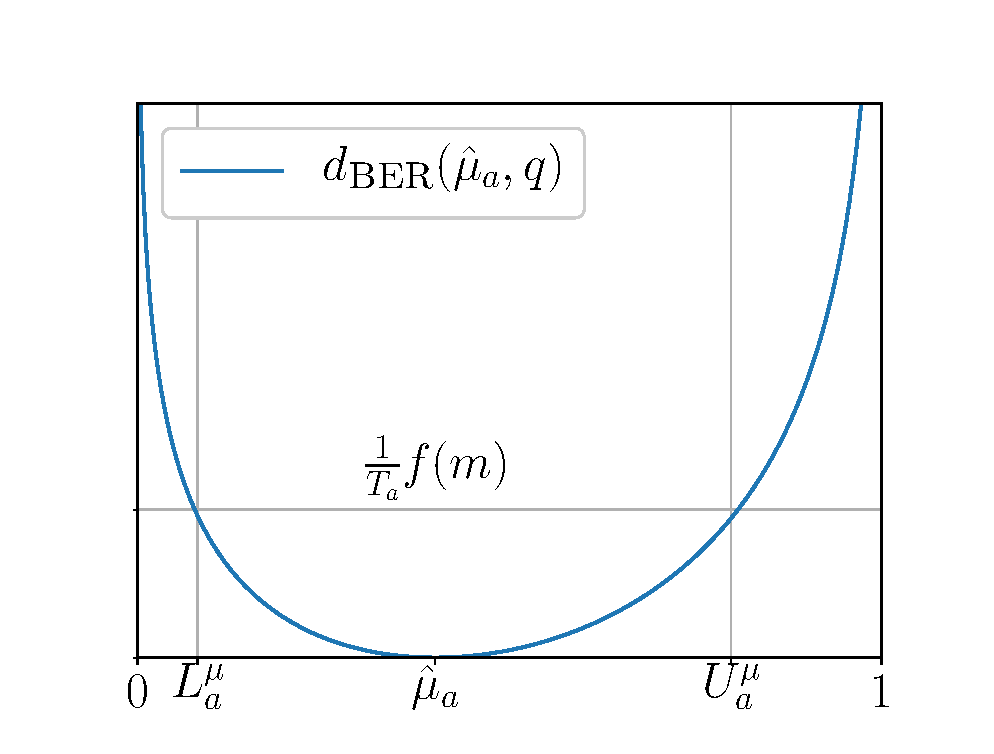
\includegraphics[width=0.6\textwidth]{img/ukl}
	\caption{The Bernoulli Kullback-Leibler divergence $\dber$, and the corresponding upper and lower confidence bounds $U^{\mu}_a$ and $L^{\mu}_a$ for the empirical average $\hat{\mu_a}$. Lower values of $f(m)$ give tighter confidence bounds that hold with lower probabilities.}
	\label{fig:ukl}
\end{figure}

$U^{\mu}_a(m)$ and $L^{\mu}_a(m)$ can be efficiently computed using Newton iterations, as for any $p\in[0, 1]$ the function $q \rightarrow \dber(p,q)$ is strictly convex and increasing (resp. decreasing) on the interval [p, 1] (resp. [0, p]).

Moreover, we use the constant function $f_2: m \rightarrow 2 \log M + 2 \log\log M$. This choice is justified in the end of section \ref{sec:regret-proof}. Because $f_2$ is lower than $f_4$, the Figure \ref{fig:ukl} shows that the bounds are tighter and hence less conservative than that of \OLOP, which should increase the performance, provided that their associated probability of violation does not invalidate the regret bound of \OLOP.


\begin{remark}[Upper bounds sharpening]
	\label{rmk:sharpen}
	\begin{leftbar}[remarkbar]
	The introduction of the B-values $B_a(m)$ was made necessary in \OLOP by the use of Chernoff-Hoeffding confidence bounds which are not guaranteed to belong to [0, 1]. On the contrary, we have in \KLOLOP that $U^\mu_a(m) \in I = [0,1]$ by construction. By Lemma \ref{lemma:seq_values}, the upper bounds sharpening step in line \ref{alg:b_values_compute} of Algorithm \ref{algo:kl-olop} is now superfluous as we trivially have $B_a(m) = U_a(m)$ for all $a\in A^L$.
	\end{leftbar}
\end{remark}

\subsection{Sample complexity}
\label{sec:sample-complexity}

We say that $u_n = \tilde{O}(v_n)$ if there exist $\alpha, \beta >0$ such that $u_n \leq \alpha \log(v_n)^\beta v_n$.
Let us denote the proportion of near-optimal nodes $\kappa_2$ as:


\begin{equation*}
\label{eq:kappa}
\kappa_2 \eqdef \limsup_{h\rightarrow\infty}{\left|\left\{a\in a^H:V(a) \geq V - 2\frac{\gamma^{h+1}}{1-\gamma}\right\}\right|^{1/h}}
\end{equation*}

\begin{theorem}[Sample complexity]
	\label{thm:regret}
	\begin{leftbar}[theorembar]
	We show that \KLOLOP enjoys the same asymptotic regret bounds as \OLOP. More precisely, for any $\kappa' > \kappa_2$, \KLOLOP satisfies:
	
	
	\begin{equation*}
	\expectedvalue r_n = \begin{cases}
	\tilde{0}\left(n^{-\frac{\log 1/\gamma}{\log \kappa'}}\right), & \text{if}\ \gamma\sqrt{\kappa'} > 1 \\
	\tilde{0}\left(n^{-\frac{1}{2}}\right), & \text{if}\ \gamma\sqrt{\kappa'} \leq 1
	\end{cases}
	\end{equation*}
	\end{leftbar}
\end{theorem}

\subsection{Time and memory complexity}
\label{sec:time-complexity}

After having considered the sample efficiency of \OLOP and \KLOLOP, we now turn to study their time and memory complexities. We will only mention the case of \KLOLOP for ease of presentation, but all results easily extend to \OLOP.

The Algorithm \ref{algo:kl-olop} requires, at each episode, to compute and store in memory of the reward upper-bounds and U-values of all nodes in the tree $\Tau = \sum_{h=0}^L A^h$.
Hence, its time and memory complexities are 
\begin{equation}
C(\KLOLOP) = O(M|\Tau|) = O(MK^L).
\end{equation}

The curse of dimensionality brought by the branching factor $K$ and horizon $L$ makes it intractable in practice to actually run \KLOLOP in its original form even for small problems. However, most of this computation and memory usage is wasted, as with reasonable sample budgets $n$ the vast majority of the tree $\Tau$ will not be actually explored and hence does not hold any valuable information.

We propose in Algorithm \ref{algo:lazy-kl-olop} a lazy version of \KLOLOP which only stores and processes the explored subtree, as shown in Figure \ref{fig:tree}, while preserving the inner workings of the original algorithm.

\begin{figure}[ht]
	\centering
	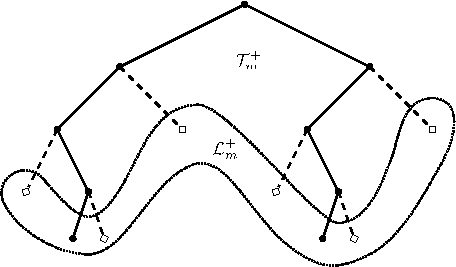
\includegraphics[width=0.6\textwidth]{img/tree_svg-tex}
	\caption{A representation of the tree $\Tau_m^+$, with $K = 2$ actions and after episode $m = 2$, when two sequences have been sampled. They are represented with solid lines and dots \textbullet, and they constitute the explored subtree $\Tau_m$. When extending $\Tau_m$ with the missing children of each node, represented with dashed lines and diamonds $\diamond$, we obtain the full extended subtree $\Tau_m^+$. The set of its leaves is denoted $\LL_m^+$ and shown as a dotted set.}
	\label{fig:tree}
\end{figure}

\begin{algorithm}[tp]
	\DontPrintSemicolon
	Let $M$ be the largest integer such that $M \log M/(2 \log 1/\gamma) \leq n$\;
	Let $L = \log M / (2 \log 1/\gamma)$\;
	Let $\Tau_0^+ = \LL_0^+ = \{\emptyset\}$\;
	\For{each episode $m = 1, \cdots, M$}{
		Compute $U_a(m-1)$ from \eqref{eq:Ua} for all $a\in\Tau_{m-1}^+$\;
		Compute $B_a(m-1)$ from \eqref{eq:Ba} for all $a\in \LL_{m-1}^+$\;
		Sample a sequence with highest B-value: $a \in \argmax_{a\in \LL_{m-1}^+} B_a(m-1)$\;
		Choose an arbitrary continuation $a^m \in aA^{L-|a|}$\tcp*{e.g. uniformly}
		Let $\Tau_m^+ = \Tau_{m-1}^+$ and $\LL_m^+ = \LL_{m-1}^+$\;
		\For{$t=1, \cdots, L$}{
			\If{$a^m_{1:t} \not \in \Tau_{m}^+$}{
				Add $a^m_{1:t-1}A$ to $\Tau_{m}^+$ and $\LL_{m}^+$\;
				Remove $a^m_{1:t-1}$ from $\LL_{m}^+$
			}
		}
	}
	\Return the most played sequence $a(n) \in \argmax_{a\in \LL_m^+} T_a(M)$
	\caption{Lazy Open Loop Optimistic Planning}
	\label{algo:lazy-kl-olop}
\end{algorithm}

\begin{theorem}[Consistency]
	\label{thm:consistency}
	\begin{leftbar}[theorembar]
	The set of sequences returned by Algorithm \ref{algo:lazy-kl-olop} is the same as the one returned by Algorithm \ref{algo:kl-olop}.
	In particular, Algorithm \ref{algo:lazy-kl-olop} enjoys the same regret bounds as in Theorem \ref{thm:regret}.
	\end{leftbar}
\end{theorem}

\begin{proposition}[Time and memory complexity]
	\begin{leftbar}[propositionbar]
	Algorithm \ref{algo:lazy-kl-olop} has time and memory complexities of:
	\begin{equation*}
	C(\texttt{Lazy KL-OLOP}) = O(KLM^2)
	\end{equation*}
	
	The corresponding complexity gain compared to the original Algorithm \ref{algo:kl-olop} is: 
	\begin{equation*}
	\frac{C(\texttt{Lazy KL-OLOP})}{C(\KLOLOP)} = \frac{n}{K^{L-1}}
	\end{equation*}
	which highlights that only a subtree corresponding to the sample budget $n$ is processed instead of the search whole tree $\Tau$.
	\end{leftbar}
\end{proposition}
\begin{proof}
	At episode $m = 1, \cdots, M$, we compute and store in memory the reward upper-bounds and U-values of all nodes in the subtree $\Tau_m^+$. Moreover, the tree $\Tau_m^+$ is constructed iteratively by adding K nodes at most L times at each episode from 0 to $m$. Hence, $|\Tau_m^+| = O(mKL)$.
	This yields directly $C(\texttt{Lazy KL-OLOP}) = \sum_{m=1}^M O(mKL) = O(M^2KL)$.
\end{proof}

\subsection{Proof of Theorem \ref{thm:regret}}
\label{sec:regret-proof}


We follow step-by step the pyramidal proof of \citep{Bubeck2010}, and adapt it to the Kullback-Leibler upper confidence bound. The adjustments resulting from the change of confidence bounds are \diff{highlighted}. The proofs of lemmas which are not significantly altered are listed in the Supplementary Material. 

We start by recalling their notations.
Let $1 \leq H \leq L$ and $a^* \in A^L$ such that $V(a^*) = V$.
Considering sequences of actions of length $1 \leq h \leq H$, we define the subset $\mathcal{I}_h$ of near-optimal sequences and the subset $\mathcal{J}$ of sub-optimal sequences that were near-optimal at depth $h-1$:
\begin{equation*}
\mathcal{I}_h = \left\{a \in A^h: V - V(a) \leq 2\frac{\gamma^{h+1}}{1-\gamma}\right\}, \mathcal{J}_h = \left\{a \in A^h: a_{1:h-1} \in \mathcal{I}_{h-1} \text{ and } a \not\in \mathcal{I}_h\right\}
\end{equation*}

By convention, $\mathcal{I}_0 = \{\emptyset\}$. From the definition of $\kappa_2$, we have that for any $\kappa'>\kappa_2$, there exists a constant C such that for any $h \geq 1$,
%\begin{equation*}
$|\mathcal{I}_h| \leq C {\kappa'}^h$
%\end{equation*}
Hence, we also have $|\mathcal{J}_h| \leq K|\mathcal{I}_{h-1}| = O({\kappa'}^h)$.

Now, for $1\leq m \leq M$, $a \in A^t$ with $t \leq h$, $h'<h$, we define the set $\mathcal{P}^a_{h,h'}(m)$ of suffixes of $a$ in $\mathcal{J}_h$ that have been played at least a certain number of times:
\begin{equation*}
\mathcal{P}^a_{h,h'}(m) = \left\{ b\in a A^{h-t}\cap \mathcal{J}_h : T_b(m) \geq \diff{2f(m)}(h+1)^2\gamma^{2(h'-h+1)} + 1 \right\}
\end{equation*}

and the random variable:

\begin{equation*}
\tau^a_{h,h'}(m) = \mathbbm{1}\{T_a(m-1) < \diff{2f(m)}(h+1)^2\gamma^{2(h'-h+1)} + 1 \leq T_a(m)\}
\end{equation*}

\begin{lemma}[Regret and sub-optimal pulls]
	\label{lemma:expected-regret}
	\begin{leftbar}[lemmabar]
	The following holds true:
	\begin{equation*}
	r_n \leq \frac{2K \gamma^{H+1}}{1-\gamma} +\frac{3K}{M}\sum_{h=1}^H\sum_{a\in\mathcal{J}_h}\frac{\gamma^h}{1-\gamma}T_a(M)
	\end{equation*}
	\end{leftbar}
\end{lemma}


The rest of the proof is devoted to the analysis of the term $\expectedvalue \sum_{a\in \mathcal{J}_h} T_a(M)$. The next lemma describes under which circumstances a suboptimal sequence of actions in $\mathcal{J}_h$ can be selected.

\begin{lemma}[Conditions for sub-optimal pull]
	\label{lemma:sub-optimal-pull}
	\begin{leftbar}[lemmabar]
	Assume that at step $m+1$ we select a sub-optimal sequence $a^{m+1}$: there exist $0 \leq h \leq L,  a\in \mathcal{J}_h$ such that $a^{m+1} \in aA^*$. Then, it implies that one of the following propositions is true:
	\begin{equation}
	\label{eq:cond-ukl}
	\tag{UCB violation}
	\diff{U_{a^*}(m)} < V,
	\end{equation}
	or
	\begin{equation}
	\tag{LCB violation}
	\label{eq:cond-lkl}
	\sum_{t=1}^h \gamma^t \diff{L^{\mu}_{a_{1:t}}(m)} \geq V(a),
	\end{equation}
	or
	\begin{equation}
	\tag{Large CI}
	\label{eq:cond-dkl}
	\sum_{t=1}^h \gamma^t\diff{\left(U^{\mu}_{a_{1:t}}(m) - L^{\mu}_{a_{1:t}}(m)\right)} > \frac{\gamma^{h+1}}{1-\gamma}
	\end{equation}
	\end{leftbar}
\end{lemma}
\begin{proof}
	As $a^{m+1}_{1:h} = a$ and \diff{because the U-values are monotonically increasing along sequences of actions} (see Remark \ref{rmk:sharpen} and Lemma \ref{lemma:seq_values}), we have $U_a(m) \geq U_{a^{m+1}}(m)$. Moreover, by Algorithm \ref{algo:kl-olop}, we have $a^{m+1} = \argmax_{a \in A^L}  U_a(m)$ and $a^*\in A^L$, so $U_{a^{m+1}}(m) \geq U_{a^*}(m)$ and finally $U_a(m) \geq U_{a^*}(m)$.
	
	Assume that \eqref{eq:cond-ukl} is false, then:
	\begin{equation}
	\label{eq:ukl-verifie}
	\sum_{t=1}^h \gamma^t U^{\mu}_{a_{1:t}}(m) + \frac{\gamma^{h+1}}{1-\gamma} = U_a(m) \geq U_{a^*}(m) \geq V
	\end{equation}
	Assume that \eqref{eq:cond-lkl} is false, then:
	\begin{equation}
	\label{eq:lkl-verifie}
	\sum_{t=1}^h \gamma^t L^{\mu}_{a_{1:t}}(m) < V(a),
	\end{equation}
	By taking the difference \eqref{eq:ukl-verifie} - \eqref{eq:lkl-verifie}, 
	\begin{equation*}
	\sum_{t=1}^h \gamma^t \left(U^{\mu}_{a_{1:t}}(m) - L^{\mu}_{a_{1:t}}(m)\right) + \frac{\gamma^{h+1}}{1-\gamma} > V - V(a)
	\end{equation*}
	But $a \in \mathcal{J}_h$, so $V - V(a) \geq \frac{2\gamma^{h+1}}{1-\gamma}$, which yields \eqref{eq:cond-dkl} and concludes the proof.
\end{proof}

\diff{In the following lemma, for each episode $m$ we bound the probability of \eqref{eq:cond-ukl} or \eqref{eq:cond-lkl} by a desired confidence level $\delta_m$, whose choice we postpone until the end of this proof. For now, we simply assume that we picked a function $f$ that satisfies $f(m)\log (m) e^{-f(m)} = O(\delta_m)$. We also denote $\Delta_M = \sum_{m=1}^{M}\delta_m$.}

\begin{lemma}[Boundary crossing probability]
	\label{lemma:boundary-crossing-prob}
	\begin{leftbar}[lemmabar]
	The following holds true, for any $1 \leq h \leq L$ and $m \leq M$,
	\begin{equation*}
	\probability{\text{\eqref{eq:cond-ukl} or \eqref{eq:cond-lkl} is true}} = \diff{O((L+h)\delta_m)}
	\end{equation*}
	\end{leftbar}
\end{lemma}
\begin{proof}
	Since $V \leq \sum_{t=1}^h \gamma^t \mu(a^*_{1:t}) + \frac{\gamma^{h+1}}{1-\gamma}$, we have,
	\begin{align*}
	\probability{\eqref{eq:cond-ukl}} &=  \probability{U_{a^*}(m) \leq V}\\
	&= \probability{\sum_{t=1}^L \gamma^t U^{\mu}_{a^*_{1:t}}(m) \leq \sum_{t=1}^L \gamma^t \mu(a^*_{1:t})}\\
	&\leq \probability{\exists 1\leq t \leq L : U^{\mu}_{a^*_{1:t}}(m) \leq \mu(a^*_{1:t})} \\
	&\leq \sum_{t=1}^L\probability{U^{\mu}_{a^*_{1:t}}(m) \leq \mu(a^*_{1:t})}
	\end{align*}
	
	\diff{In order to bound this quantity, we reduce the question to the application of a deviation inequality. For all $1\leq t\leq L$, we have on the event $\{U^{\mu}_{a^*_{1:t}}(m) \leq \mu(a^*_{1:t})\}$ that $\hat{\mu}_{a^*_{1:t}}(m) \leq U^{\mu}_{a^*_{1:t}}(m) \leq \mu(a^*_{1:t}) < 1$. Therefore, for all $0 < \delta < 1 - \mu(a^*_{1:t})$, by definition of $U^{\mu}_{a^*_{1:t}}(m)$:}
	
	\begin{equation*}
	\diff{d(\hat{\mu}_{a^*_{1:t}}(m), U^{\mu}_{a^*_{1:t}}(m)+\delta) > \frac{f(m)}{T_{a^*_{1:t}}(m)}}
	\end{equation*}
	
	\diff{As $d$ is continuous on $(0,1)\times[0, 1]$, we have by letting $\delta \rightarrow 0$ that:}
	
	\begin{equation*}
	\diff{d(\hat{\mu}_{a^*_{1:t}}(m), U^{\mu}_{a^*_{1:t}}(m)) \geq \frac{f(m)}{T_{a^*_{1:t}}(m)}}
	\end{equation*}
	
	\diff{Since d is non-decreasing on $[\hat{\mu}_{a^*_{1:t}}(m), \mu(a^*_{1:t})]$,}
	
	\begin{equation*}
	\diff{d(\hat{\mu}_{a^*_{1:t}}(m), \mu(a^*_{1:t})) \geq d(\hat{\mu}_{a^*_{1:t}}(m), U^{\mu}_{a^*_{1:t}}(m)) \geq \frac{f(m)}{T_{a^*_{1:t}}(m)}}
	\end{equation*}
	
	\diff{We have thus shown the following inclusion:}
	
	\begin{equation*}
	\diff{\{U^{\mu}_{a^*_{1:t}}(m) \leq \mu(a^*_{1:t})\} \subseteq \left\{ \mu(a^*_{1:t}) > \hat{\mu}_{a^*_{1:t}}(m) \text{ and } d(\hat{\mu}_{a^*_{1:t}}(m), \mu(a^*_{1:t})) \geq \frac{f(m)}{T_{a^*_{1:t}}(m)} \right\}}
	\end{equation*}
	
	\diff{Decomposing according to the values of $T_{a^*_{1:t}}(m)$ yields:}
	
	\begin{equation*}
	\diff{\{U^{\mu}_{a^*_{1:t}}(m) \leq \mu(a^*_{1:t})\} \subseteq \bigcup_{n=1}^m \left\{ \mu(a^*_{1:t}) > \hat{\mu}_{a^*_{1:t}, n} \text{ and } d(\hat{\mu}_{a^*_{1:t}, n}, \mu(a^*_{1:t})) \geq \frac{f(m)}{n} \right\}}
	\end{equation*}
	
	\diff{We now apply the deviation inequality provided in Lemma 2 of Appendix A in \citep{Cappe2013}: $\forall \epsilon > 1$, provided that $0 < \mu(a^*_{1:t}) < 1$,}
	
	\begin{equation*}
	\diff{\probability{\bigcup_{n=1}^m \left\{ \mu(a^*_{1:t}) > \hat{\mu}_{a^*_{1:t}, n} \text{ and } n \dber(\hat{\mu}_{a^*_{1:t}, n}, \mu(a^*_{1:t})) \geq \epsilon \right\}} \leq e\ceil{\epsilon \log m}e^{-\epsilon}\,.}
	\end{equation*}
	
	\diff{By choosing $\epsilon = f(m)$, it comes}
	\begin{align*}
	\diff{\probability{\eqref{eq:cond-ukl}} \leq \sum_{t=1}^L e\ceil{f(m)\log m}e^{-f(m)} = O(L\delta_m)}
	\end{align*}
	
	The same reasoning gives: $\quad\displaystyle{
		\probability{\eqref{eq:cond-lkl}} = \diff{O(h\delta_m)}}$.
\end{proof}

\begin{lemma}[Confidence interval length and number of plays]
	\label{lemma:ci-length}
	\begin{leftbar}[lemmabar]
	Let $1 \leq h \leq L$, $a\in \mathcal{J}_h$ and $0 \leq h' < h$. Then  \eqref{eq:cond-dkl} is not satisfied if the following propositions are true:
	\begin{equation}
	\label{eq:sampled-enough-h}
	\forall 0\leq t\leq h', T_{a_{1:t}}(m) \geq \diff{2f(m)}(h+1)^2\gamma^{2(t-h-1)}
	\end{equation}
	and
	\begin{equation}
	\label{eq:sampled-enough}
	T_{a}(m) \geq \diff{2f(m)}(h+1)^2\gamma^{2(h'-h-1)}
	\end{equation}
	\end{leftbar}
\end{lemma}
\begin{proof}
	We start by providing an explicit upper-bound for the length of the confidence interval $U^{\mu}_{a_{1:t}} - L^{\mu}_{a_{1:t}}$. \diff{By Pinsker's inequality:}
	
	\begin{equation*}
	\diff{\dber(p, q) > \dquad(p, q)}
	\end{equation*}
	
	\diff{Hence for all $C>0$, }
	\begin{equation*}
	\diff{\dber(p, q) \leq C   \implies 2(q - p)^2 < C  \implies p - \sqrt{C/2} < q < p + \sqrt{C/2}}
	\end{equation*}
	\diff{And thus, for all $b\in A^*$, by definition of $U^{\mu}$ and $L^{\mu}$:}
	\begin{align*}
	\diff{U^{\mu}_{b}(m) - L^{\mu}_{b}(m) \leq \frac{S_b(m)}{T_b(m)} + \sqrt{\frac{f(m)}{2T_b(m)}} -  \left(\frac{S_b(m)}{T_b(m)} - \sqrt{\frac{f(m)}{2T_b(m)}}\right) 
		= \sqrt{\frac{2f(m)}{T_b(m)}}}
	\end{align*}
	
	Now, assume that \eqref{eq:sampled-enough-h} and \eqref{eq:sampled-enough} are true. Then, we clearly have:
	\begin{align*}
	\sum_{t=1}^h \gamma^t\left(U^{\mu}_{a_{1:t}}(m) - L^{\mu}_{a_{1:t}}(m)\right) &\leq \sum_{t=1}^{h'} \gamma^t \sqrt{\frac{2f(m)}{T_{a_{1:t}}(m)}} + \sum_{t=h'+1}^h \gamma^t \sqrt{\frac{2f(m)}{T_{a_{1:t}}(m)}} \\
	&\leq \frac{1}{(h+1)\gamma^{-h-1}} \sum_{t=1}^{h'} 1 + \frac{1}{(h+1)\gamma^{-h-1}} \sum_{t=h'+1}^h \gamma^{t-h'}  \\
	&\leq \frac{\gamma^{h+1}}{h+1} \left( h' + \frac{\gamma}{1-\gamma} \right)\leq \frac{\gamma^{h+1}}{1-\gamma}\,.
	\end{align*}
\end{proof}

\begin{lemma}
	\label{lemma:size_Ph}
	\begin{leftbar}[lemmabar]
	Let $1 \leq h \leq L,  a\in \mathcal{J}_h$ and $0\leq h'<h$. Then $\tau^a_{h,h'}=1$ implies that either equation \eqref{eq:cond-ukl} or \eqref{eq:cond-lkl} is satisfied or the following proposition is true:
	
	
	\begin{equation}
	\label{eq:P-min-size}
	\exists 1\leq t \leq h': |\mathcal{P}_{h,h'}^{a_{1:t}}(m)| < \gamma^{2(t-h')}
	\end{equation}
	\end{leftbar}
\end{lemma}

\begin{lemma}
	\label{lemma:expected-P-size}
    \begin{leftbar}[lemmabar]
	Let $1\leq h\leq L$ and $0 \leq h' < h$. Then the following holds true,
	
	\begin{equation*}
	\expectedvalue |\mathcal{P}^\emptyset_{h,h'}(M)| = \tilde{O}\left(\gamma^{-2h'}\mathbbm{1}_{h'>0}\sum_{t=0}^{h'}(\gamma^2 \kappa')^t + (\kappa')^h\diff{\Delta_M} \right).
	\end{equation*}
	\end{leftbar}
\end{lemma}

\begin{lemma}
	\label{lemma:expected-plays-count}
	\begin{leftbar}[lemmabar]
	Let $1\leq h\leq L$. The following holds true,
	\begin{equation*}
	\expectedvalue \sum_{a\in \mathcal{J}_h} T_a(M) = \tilde{O}\left(\gamma^{-2h} + \diff{(\kappa')^h(1+M\Delta_M+\Delta_M) + (\kappa'\gamma^{-2})^h\Delta_M}\right)
	\end{equation*}
	\end{leftbar}
\end{lemma}

Thus by combining Lemma \ref{lemma:expected-regret} and \ref{lemma:expected-plays-count} we obtain:
\begin{equation*}
\expectedvalue r_n = \tilde{O}\left(\gamma^H + \gamma^{-H}M^{-1} + (\kappa' \gamma)^{H}M^{-1}\diff{(1+M\Delta_M+\Delta_M)} + (\kappa')^H\gamma^{-H}M^{-1}\diff{\Delta_M}\right)
\end{equation*}
Finally,
\begin{itemize}
	\item if $\kappa'\gamma^2 \leq 1$, we take $H = \floor{\log M / (2\log 1/\gamma)}$ to obtain:
	\begin{equation*}
	\expectedvalue r_n = \tilde{O}\left(M^{-\frac{1}{2}} + M^{-\frac{1}{2}} + M^{-\frac{1}{2}}M^{\frac{\log \kappa'}{2\log 1/\gamma}} \diff{\Delta_M}\right)
	\end{equation*}
	For the last term to be of the same order of the others, we need to have $\Delta_M = O(M^{-\frac{\log \kappa'}{2\log 1/\gamma}})$. Since $\kappa'\gamma^2 \leq 1$, we achieve this by taking \diff{$\Delta_M = O(M^{-1})$}.
	\item if $\kappa'\gamma^2 > 1$, we take $H = \floor{\log M / \log \kappa'}$ to obtain:
	\begin{equation*}
	\expectedvalue r_n = \tilde{O}\left(M^{\frac{\log \gamma}{\log \kappa'}} + M^{\frac{\log \gamma}{\log \kappa'}}\diff{(1+M\Delta_M+\Delta_M)} + M^{\frac{\log 1/\gamma}{\log \kappa'}}\diff{\Delta_M}\right)
	\end{equation*}
	Since $\kappa'\gamma^2 > 1$, the dominant term in this sum is $M^{\frac{\log \gamma}{\log \kappa'}}M\Delta_M$. Again, taking \diff{$\Delta_M = O(M^{-1})$} yields the claimed bounds.
\end{itemize}
Thus, the claimed bounds are obtained in both cases as long as we can impose $\Delta_M = O(M^{-1})$, that is, find a sequence $(\delta_m)_{1\leq m\leq M}$ and a function $f$ verifying:
\begin{equation}
\sum_{m=1}^M \delta_m = O(M^{-1})\quad \text{and}\quad f(m)\log (m) e^{-f(m)} = O(\delta_m)
\end{equation}

By choosing \diff{$\delta_m = M^{-2}$ and $f(m) = 2 \log M + 2 \log\log M$}, the corresponding \KLOLOP algorithm does achieve the regret bound claimed in Theorem \ref{thm:regret}.


\section{Experiments and Conclusion}
\label{sec:planning-experiments}

We have performed some numerical experiments to evaluate and compare the following planning algorithms\footnote[1]{The source code is available at \url{https://eleurent.github.io/kl-olop/}}:
\begin{itemize}
	\item \texttt{Random}: returns a random action, we use it as a minimal performance baseline.
	\item \OPD: the \emph{Optimistic Planning for Deterministic systems} from \citep{Hren2008}, used as a baseline of optimal performance. This planner is only suited for deterministic environments, and exploits this property to obtain faster rates. However, it is expected to fail in stochastic environments.
	\item \OLOP: as described in section \ref{sec:kl-olop-olop}.\footnote[2]{Note that we use the lazy version of $\OLOP$ and $\KLOLOP$ presented in Section \ref{sec:time-complexity}, otherwise the exponential running-time would have been prohibitive.}
	\item \KLOLOP: as described in section \ref{sec:kl-olop-kl-olop}.\footnotemark[2]
	\item \texttt{KL-OLOP}(1): an aggressive version of \KLOLOP where we used $f_1(m) = \log M$ instead of $f_2(m)$. This threshold function makes the upper bounds even tighter, at the cost of an increased probability of violation. Hence, we expect this solution to be more efficient in close-to-deterministic environments. However, since we have no theoretical guarantee concerning its regret as we do with $\KLOLOP$, it might not be conservative enough and converge too early to a suboptimal sequence, especially in highly stochastic environments.
\end{itemize}

They are evaluated on the following tasks, using a discount factor of $\gamma=0.8$:
\begin{itemize}
	\item A \href{https://github.com/eleurent/highway-env/}{highway driving} environment \citep{highway-env}: a vehicle is driving on a road randomly populated with other slower drivers, and must make their way as fast as possible while avoiding collisions by choosing on the the following actions: \texttt{change-lane-left}, \texttt{change-lane-right}, \texttt{no-op}, \texttt{faster}, \texttt{slower}.
	\item A \href{https://github.com/maximecb/gym-minigrid}{gridworld} environment \citep{gym_minigrid}: the agent navigates in a randomly-generated gridworld composed of either empty cells, terminal lava cells, and goal cells where a reward of $1$ is collected at the first visit.
	\item A stochastic version of the gridworld environment with noisy rewards, where the noise is modelled as a Bernoulli distribution with a 15\% probability of error, i.e. receiving a reward of 1 in an empty cell or 0 in a goal cell.
\end{itemize}

\begin{figure}[pth]
	\centering
	\begin{subfigure}[b]{0.8\linewidth}
		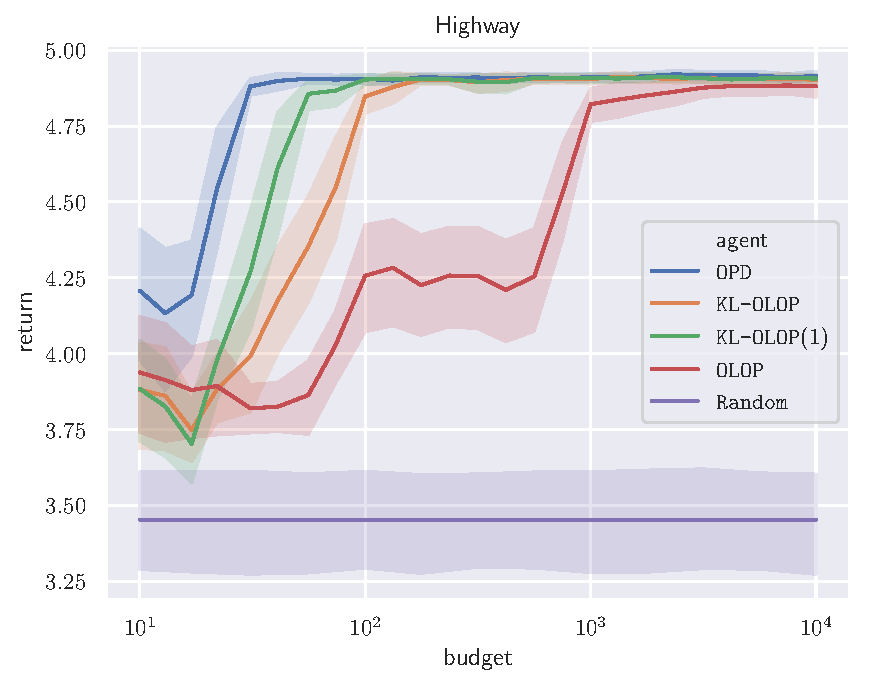
\includegraphics[width=\textwidth]{img/hw_return_svg-tex}
		\caption{Highway}
		\label{sub:highway}
	\end{subfigure}
	\newline
	\begin{subfigure}[b]{0.49\linewidth}
		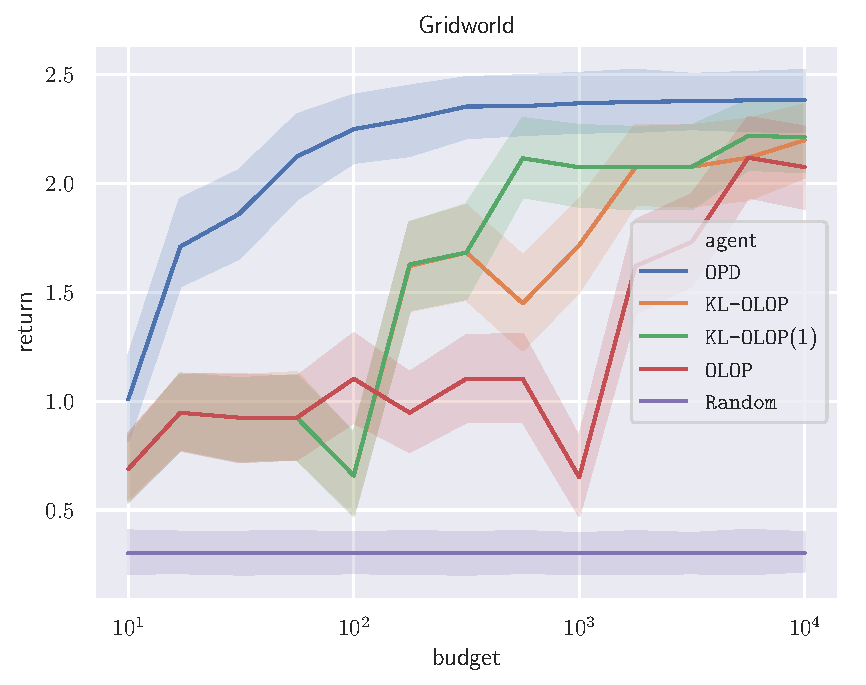
\includegraphics[width=\textwidth]{img/gw_return_svg-tex}
		\caption{Gridworld}
		\label{sub:gridworld}
	\end{subfigure}
	\begin{subfigure}[b]{0.49\linewidth}
		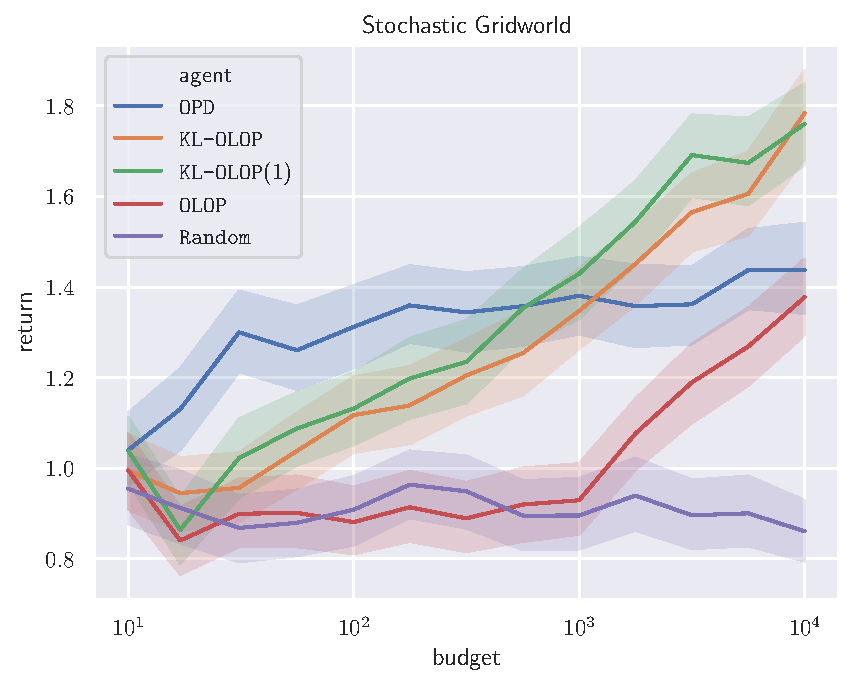
\includegraphics[width=\textwidth]{img/gw_stoch_return_svg-tex}
		\caption{Stochastic Gridworld}
		\label{sub:gridworld_stoch}
	\end{subfigure}
	\caption{Numerical experiments: for each environment-agent configuration, we compute the average return over 100 runs –- along with its 95\% confidence interval –- with respect to the available budget $n$.}
	\label{fig:experiments}
\end{figure}

\begin{figure}[pth]
	\centering
	
	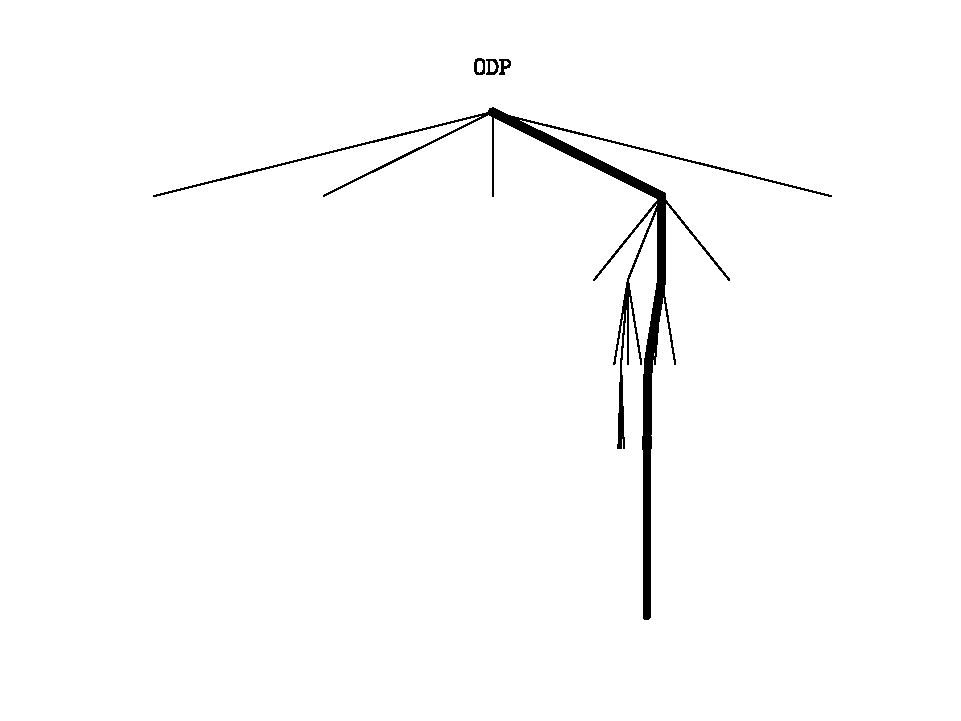
\includegraphics[width=0.6\textwidth]{img/tree_OPD_svg-tex} \includegraphics[width=0.6\textwidth]{img/tree_OLOP_svg-tex}
	\includegraphics[width=0.6\textwidth]{img/tree_KL-OLOP_svg-tex}
	
	\caption{The look-ahead trees (down to depth 6) expanded by the planning algorithms from the same initial state in the highway environment with the same budget $n=10^3$. The width of edges represents the nodes visit count $T_a(M)$.}
	\label{fig:trees}
\end{figure}

The results of our experiments are shown in Figure \ref{fig:experiments}. The \OPD algorithm converges very quickly to the optimal return in the two first environments, shown in Figure \ref{sub:highway} and Figure \ref{sub:gridworld}, because it exploits their deterministic nature: it needs neither to estimate the rewards through upper-confidence bounds nor to sample whole sequences all the way from the root when expanding a leaf, which provides a significant speedup. It can be seen as an oracle allowing to measure the conservativeness of stochastic planning algorithms. And indeed, even before introducing stochasticity, we can see that \OLOP performs quite badly on the two environments, only managing to solve them with a budget in the order of $10^{3.5}$. In stark contrast, \KLOLOP makes a much better use of its samples and reaches the same performance an order of magnitude faster. This is illustrated by the expanded trees shown in Figure \ref{fig:trees}: \OPD exploits the deterministic setting and produces a sparse tree densely concentrated around the optimal trajectory. Conversely, the tree developed by \OLOP is evenly balanced, which suggests that \OLOP behaves as uniform planning as hypothesised in Section \ref{sec:kl-olop-behaviour}. \KLOLOP is more efficient and expands a highly unbalanced tree, exploring the same regions as \OPD. Furthermore, in the stochastic gridworld environment shown in Figure \ref{sub:gridworld_stoch}, we observe that the deterministic \OPD planner's performance saturates as it settles to suboptimal trajectories, as expected. Conversely, the stochastic planners all find better-performing open-loop policies, which justifies the need for this framework. Again, \KLOLOP converges an order of magnitude faster than \OLOP. Finally, \texttt{KL-OLOP}(1) enjoys good performance overall and displays the most satisfying trade-off between aggressiveness in deterministic environments and conservativeness in stochastic environments; hence we recommend this tuning for practical use.

\subsection{Conclusion}

We introduced an enhanced version of the \OLOP algorithm for open-loop online planning, whose design was motivated by an investigation of the over-conservative search behaviours of \OLOP. We analysed its sample complexity and showed that the original regret bounds are preserved, while its empirical performances are increased by an order of magnitude in several numerical experiments. Finally, we proposed an efficient implementation that benefits from a substantial speedup, facilitating its use for real-time planning applications.

\section{State-aware planning}

\section{Experiments and Conclusion}
%!TEX root = ../../PhD_thesis__Edouard_Leurent

\chapter{Preparing for the Worst}
\label{chapter:7}

\begin{flushright}
	\begin{tabular}{@{}l@{}}
		\emph{Two roads diverges in a wood, and I--}\\
		\emph{I took the one less traveled by,}\\
		\emph{And that has made all the difference.}\\
	\end{tabular}
	
	Robert Frost, \href{https://eleurent.github.io/sisyphe/texts/the-road-not-taken.html}{\emph{The Road Not Taken}}.
\end{flushright}


\section{Confident model estimation}
\section{State interval prediction}
\section{Robust control and constraint satisfaction}

%!TEX root = ../../PhD_thesis__Edouard_Leurent.tex

\makeatletter
\def\toclevel@chapter{-1}
\makeatother

%TODO: Discussion ?
\chapter{General Conclusion and Perspectives}
\label{chapter:conclusion}

\begin{flushright}
	\begin{tabular}{@{}l@{}}
		\emph{Nos équipiers}\\
		\emph{\hspace*{1.0cm}Sur les voies}\\
		\emph{\hspace*{0.5cm}Ralentissez}\\
	\end{tabular}

	Vinci Autoroutes\footnote{Writings collected by \href{https://twitter.com/pooredward/status/1273249408231124994}
		{@pooredward}.}\hspace*{1cm}
\end{flushright}

\section{Conclusion on our contributions}
In this thesis, we proposed a learning-based approach to the problem of behavioural planning for autonomous vehicles, with a focus on situations where several drivers are interacting. Following an in-breadth (\Cref{chapter:2}) as well as in-depth (\Cref{chapter:3}) initial investigation, we identified a set of key issues which make this problem challenging. We now recall each of these subjects, and precise how we strived to address them both in the model-free approach of \Cref{part:2} and the model-based approach of \Cref{part:3}.

%TODO highlight our most significant contributions

\paragraph{Coupled social dynamics}
In dense traffic, the dynamics of distinct vehicles are locally coupled, due to how drivers react and adapt to their surroundings. Consequently, predicting the course or acting in a driving scene requires a \emph{social awareness} skill: the ability to accurately understand and exploit these couplings.
In \Cref{chapter:4}, this skill was implemented through a \emph{social attention} mechanism in the policy architecture, which enables the agent to filter out irrelevant objects from a complex driving scene and retain only those that represent a risk of collision. In \Cref{chapter:5}, this coupling was made even more implicit by describing the motion of a vehicle $i$ through a dynamical model $\dot{x_i} = f_i(x)$ hat accepts the whole traffic state $x$ as an input.

\paragraph{Uncertainty due to human drivers}
Another key difficulty lies in the uncertainty of human behaviours. In \gls{RL}, the traditional approach to account for uncertainty is to incorporate stochasticity in the system dynamics, as we did in \Cref{chapter:5} where the objectives are formulated in terms of \emph{expected} rewards and costs. Incidentally, we also observed in \Cref{chapter:4} that our attention-based architecture is highly sensitive to ambiguous and disambiguated information, such as vehicles' destinations. In \Cref{chapter:7} however, we adopted another view and assumed that the dynamics were (close to) deterministic, but dependent on some unknown parameters --both continuous and discrete-- that could be estimated along the way.

\paragraph{Safety}
To deal with this uncertainty, three models of safety have been studied. In \Cref{chapter:5}, following the \gls{CMDP} framework, we formalised risk as the expected discounted sum of an additional cost signal $\constraint(s,a)$ --separate from the rewards $\reward(s,a)$-- constrained to remain below a threshold $\budget$. In \Cref{chapter:7}, we introduced a novel interval predictor allowing us to bound the set of reachable trajectories given the current parametric uncertainty over dynamics. This enabled us to cast safety as a robust stabilisation and constraint satisfaction problem, ensuring that the systems stays at all time within a safe space $\safestates\times\safecontrols$. Finally, to go beyond stabilisation problems, we considered a third formalisation of safety as a worst-case outcome, and proposed an algorithm for the minimax control of a generic reward function $\R(s,a)$.

\paragraph{Trade-off between safety and efficiency}
As we've just seen, safety is always defined with respect to some \emph{admissible} uncertainty. The larger the set of scenarios one is willing to consider and protect against, the more conservative they need to be to ensure safety. In particular, situations that require interacting with other agents are always susceptible to lead to accidents, when considering unlikely adversarial scenarios. In that sense, \emph{absolute safety is not achievable}, or only at the cost of usability. To strike the right level of safety, we need to consider the right level of uncertainty, the right set of outcomes. In \Cref{chapter:7}, the size of this ambiguity set to protect against can be controlled by adjusting the confidence level $\delta$ for continuous parameters (\eg driving style), and by adding or removing $(A,\phi)$-modelling assumptions from the multi-model extension, for discrete parameters (\eg potential destinations or lanes for a vehicle). In \Cref{chapter:5}, we embrace this trade-off even more explicitly. Rather than trying to adjust the scope and size of the uncertainty at its source, we instead directly control its effects on both the efficiency (rewards) of the policy and its safety (costs), by training a \emph{budgeted} policy $\budgetedpolicy$ that takes as input the desired level of risk $\confidence$.

\paragraph{Sample efficiency}
As for most reinforcement learning problems, we were concerned by minimising the number of samples required to reach optimality. To that end, we exploited the specificities and structures of the behavioural planning problem in several ways. In \Cref{chapter:4}, we embedded an inductive bias into the policy architecture by enforcing its invariance to permutations of the scene description, and observed that this fosters faster learning. In \Cref{chapter:7}, some structure was similarly imposed, on the dynamics model this time, in the form of a parametrised linear model which allowed to significantly reduce the dimension of the hypothesis space. We were also able to provide a bound on the simple regret relating the agent performance to the number of observed transition samples. In \Cref{chapter:6}, we looked into the sample efficiency of the planning procedure, and specifically tree-based planning algorithms. First, in the case of stochastic dynamics representing human behaviours, we proposed a modification of the \OLOP algorithm that improves its empirical sample complexity by an order on magnitude, while retaining its theoretical guarantees. Second, we showed that merging similar nodes in the lookahead tree enables to decrease the near-optimal branching factor featured in the regret bound of the algorithm. This translated as substantial empirical improvements in simple path planning tasks, where distinct sequences of actions lead to overlapping trajectories.


\section{Outstanding issues and perspectives}

In this section, I will adopt a more personal and subjective standpoint, and discuss which are the main barriers between research and industrialisation. Indeed, though we never intended for this thesis to lead directly to products, practical applications remains the long haul goal that motivates our work, and I must now examine our contributions again in this light.

A first and general concern of mine is that, beside the warm comfort of the well-behaved theoretical frameworks in which we place ourselves, the sheer complexity of the real world can be overwhelming. While any single aspect --partial observability, temporal abstraction, non-stationarity, risk aversion, you name it-- can be isolated and studied independently, the question of how to merge all these approaches into one single integrated product seems arduous, if not hopeless. Yet, any candidate algorithm not addressing any of these issues would be unfit.
In the sequel, I will not be so ambitious but reflect instead on a more reasonable question: are the methods that we developed likely to be suitable for a real-world application?

\paragraph{Reinforcement Learning in continuous states}

Let us start by our work in \Cref{part:2}. Following a model-free perspective in continuous states, we resorted function approximation using neural networks. Unfortunately, Deep Learning interacts with Reinforcement Learning algorithms in ways that are yet to be understood, but already infamous for their brittleness. In \Cref{chapter:4}, even our best policies after training still suffer a prohibitive rate of collisions of \SI{5}{\per}, considerably higher than the required performances. 
As we discussed, this may be attributed to the reward function that would not penalise collisions enough, but reward engineering is tedious and might in turn lead to over-conservative policies. The budgeted approaches of \Cref{chapter:5} were meant to address this issue, but at the price of an increased complexity, and our negative result of \Cref{thm:contraction} raises concerns over convergence in the general case. 
Another concern lies in our use of a very naive exploration policy --the $\epsilon$-greedy-- which takes random actions at a fixed frequency, a strategy widely considered as inefficient and damaging, yet which we had no choice but resorting to in the absence of a better solution. Guided exploration strategies tailored for regret minimisation, and especially following the \gls{OFU} principle, have been studied in the context of finite state-action spaces \citep{Auer2009,Azar2017}. 
These methods typically require the ability of counting the number of state visits, the question of how they can be extended to continuous spaces constitutes a promising research perspective. First steps have recently been made in that direction, by either relying on approximated \emph{pseudo-counts} \citep{Guyon2017}, or by deriving similar regret bounds under linear function approximation \citep{Jin2020}.

\paragraph{Trial without error?}

% In this thesis, we tried to solve behavioural planning in simulation, as a necessary step to solve it in real world. Thus treated simulation as our target task. 
Assume for a moment that the research community was able to solve the aforementioned problem and came up with exciting new algorithms for continuous state space with promising regret bounds. There remains an inevitable and fatal limitation: \emph{the foundations of \glsxtrlong{RL} are intrinsically based on trial and error}. Unfortunately, this is not an acceptable paradigm for the development of safety-critical problems such as \glsxtrlong{AD}. For reference, when we applied the model-free methods of \Cref{part:2} to very simple tasks, they converged in about 50k interaction samples, which represents about \SI{15}{\hour} of driving. Throughout training, the agents experienced about two thousand collisions. More generally, having vehicles \emph{exploring} on the roads among human drivers is morally inconceivable. Is there any chance at all to come up with learning algorithms that do not require actually causing accidents while training?

\paragraph{Safety guarantees}

As a first candidate, the line of work of Safe Control is committed to develop algorithms that are guaranteed never to reach an unsafe state, or with a provably bounded probability of failure. 
Likewise, in \Cref{chapter:7}, we managed to obtain some theoretical guarantees: a robust constraint satisfaction result, and a lower-bound on the worst-case outcome, that increases towards near-optimal performance with the number of samples. However, it is evident that these results are worth as much as their underlying assumptions, which could be: not much. Indeed, it seems very dubious that the complexity of human behaviours can be accurately described by our linear dynamics \Cref{assumpt:structure}, and our own proposed system largely overlooks large parts of the driving task. With \Cref{assumpt:feasible-constr}, the safe region $\safestates$ cannot be chosen freely, but must contain the basin of attraction $\safestates_{f}$ whose size grows with uncertainty. Finally, the assumptions of \Cref{thm:control-error} do not hold even in our simple simulations: the behaviours of observed vehicles are not persistently excited (\ie constantly braking before their leading vehicle and changing lanes). More generally, safety analyses can never protect against unmodeled events: a tree or a package falling down the road. Yet, having to model the world is daunting, especially since theoretical analysis imposes an additional constraint on the modelling effort, often at the expense of empirical performance. This may explain why practical achievements often precede their formal analysis. In the end, do we prefer relying on a simpler model that we can analyse under some assumptions unlikely to hold in practice, or more complex black-box models which tend to perform better on experimental benchmarks? Fortunately, all is not bleak and it has been observed in countless occasions that even when the guarantees do not hold, the founding principles of an algorithm can lead to designs that still exhibit the desired properties, and can robustly generalise. An example is the reliable of control systems in the aerospace industry, which even though aircraft dynamics are not \emph{really} linear and measurement noises are not \emph{really} Gaussian.

% TODO: still, current safety frameworks are not well suited to AD. Stabilisation: meh. Safe states: meh.
% Perspective: investigate new ones (which ?)
% But always the same problem: guaranteed protection against rare events = conservativeness.

\paragraph{Simulation and beyond?}

Another obvious way to avoid trial-and-error in the real world is to rely on simulation. Of course, the effort of modelling a complex world remains, but dropping the analysability requirement significantly relaxes the constraints on how this description can be expressed. We can safely expect that simulations will continue to play an increasingly significant part in \gls{AD} technologies, for both offline pre-training and online planning. This can be the occasion to divert our research efforts from the traditional regret minimisation objective, which does not make much sense in a simulated environments where rewards are free but samples are costly. In contrast, a promising research direction is the study of the more appropriate Pure Exploration setting, which aims at relating the policy suboptimality to the number of samples. I already took part in collaborations exploring this direction \citep{Jonsson2020planning,Kaufmann2020adaptive,Menard2020Fast} and hope to pursue this path further. 
Finally, relying on simulation introduces the additional question of how to adapt knowledge from simulation to the real world. A fine-tuning training process in real conditions would involve experiencing real failures again, though hopefully in reduced numbers, which could be realistic under human interventions \citep{Saunders2018,Kendall2019}. Another path of interest to me could be to leverage offline \gls{RL} methods \citep{Thomas2015,Laroche2019}, that could enable to safely improve pre-trained policies around nominal states in a dataset of real driving data.
